\chapter{Protective Scheduling for distributed Job Execution}
\label{ch:PFSP}
% \lipsum[50]
In this chapter, we focus on developing scheduling policies that improve job processing efficiency in terms of average job response time, while guaranteeing a certain criterion of long-term fairness for online distributed job execution, where each job's workload is distributed across multiple sites. Inspired by the concept of protective scheduling in the single site system introduced by Friedman \textit{et al.} \cite{friedman2003fairness, friedman2003protective}, our long-term fairness criterion dictates that no job should complete later than it would under a distributed Processor Sharing (PS) protocol, which evenly shares the site capacity among all active jobs at each site. Building on this foundation, we aim to develop job scheduling algorithms that tackle the dual challenges of enhancing processing efficiency while strictly adhering to this fairness criterion.


\section{Preliminaries}
\label{sec:prelim}
\subsection{Slack System in Single-Site Case}
\label{sec:pre_slack}

We introduce a slack system that provides an intuitive protectiveness assessment of the current system state, identifying whether any jobs are projected to exceed their completion times under the Processor Sharing (PS) policy. It is defined as follows \cite{friedman2003protective}:

Consider a single-site system with compute resources, where the total resource capacity is assumed to be $1$ for simplicity. During execution, the system hypothetically runs a Processor Sharing (PS) policy to obtain each job's PS completion time, which serves as its deadline. Every job in the system has two types of job loads, namely the real load and the PS load, which represent the remaining load of a job in the current system and the hypothetical PS execution respectively. Initially, the real load and the PS load of a new job are both equal to its initial load upon its arrival. The PS load then continuously decreases according to a simulated execution of the PS policy, where processing capacity is evenly shared by all jobs with positive loads, while its real load remains unchanged or decreases according to the actual scheduling policy. Let the current real loads and PS loads for $n$ jobs in the system be $w_1, w_2, \dots, w_n$ and $v_1, v_2, \dots, v_n$, respectively. For simplicity, the job sequence is sorted in ascending order of their PS loads, i.e., $v_1 \le v_2 \le \dots \le v_n$ (note that the PS load order is identical to the PS completion time order of the jobs). The slack of a job $J_i$ is computed as follows:
\begin{equation}
    \label{eq:slack_single}
    s_i = \sum_{l=1}^{i} v_{l} + (n-i)v_i- \sum_{l=1}^i w_l.
\end{equation}
Specifically, the slack $s_i$ consists of two parts: (i) the PS completion time of $J_i$, given by $\sum_{l=1}^{i} v_{l} + (n-i)v_i$, and (ii) the time required to complete the real loads of the first $i$ jobs, given by $\sum_{l=1}^i w_l$. Consequently, $s_i$ quantifies the maximum permissible delay for $J_i$ and its preceding jobs to complete before violating the deadline set at $J_i$'s PS completion time.

\subsection{Two Types of Events in Slack System}
\label{sec:Pre_TwoEvents}
We now explain how the slack system will change under various events. Friedman \textit{et al.} \cite{friedman2003protective} discussed the changes of the slack system under two types of events. First, if the system serves some job $J_i$ for a duration of $\Delta t$, the slacks of jobs preceding $J_i$ in the PS load order will decrease by $\Delta t$:
\begin{equation}
    s_l = s_l -\Delta t,\quad \forall l \in \{1, \dots, i-1\}.
\end{equation}
Second, if a new job arrives in the system and joins in the job sequence at the $i$-th position based on its PS load (suppose its initial load is $x$), it will cause the slacks of jobs preceding it to increase by $x$:
\begin{equation}
    s_l = s_l + x,\quad \forall l \in \{1, \dots, i-1\}.
\end{equation}
For both events, the slacks of subsequent jobs $J_{i+1}, J_{i+2}, \dots, J_n$ remain unchanged. 

\subsection{Servable and Completable jobs}
Friedman \textit{et al.} \cite{friedman2003protective} proved that a scheduling policy is protective if and only if the slack of each job remains non-negative at all times. In other words, once the slack of any job becomes negative, then regardless of subsequent scheduling decisions (in the absence of new job arrivals), at least one job will inevitably complete later than its completion time under the PS policy. Therefore, the analysis of the first type of event above (serving jobs) indicates that it may not be true that all jobs can be prioritized for processing immediately if the system aims to maintain protectiveness. This fundamental restriction introduces the concept of servability and completability. %Without loss of generality, we assume that the job sequence is sorted in ascending order of their PS loads: %For simplicity, in the following definition we assume that the job sequence is already sorted based on their PS loads.

%Consequently, avoiding negative slack implies that not all jobs can be prioritized for execution if the system aims to maintain protectiveness. This restriction naturally motivates the concepts of servability and completability. Without loss of generality, we assume that the job sequence is indexed in ascending order of their PS loads.

\begin{definition}
    A job $J_i$ is \textbf{servable} if and only if $s_{l} > 0$ for all $l \in \{1, \dots, i-1\}$.
\end{definition}

\begin{definition}
    A job $J_i$ is \textbf{completable} if and only if $s_{l} \ge w_{i}$ for all $l \in \{1, \dots, i-1\}$.
\end{definition}

%Note that the first job in the PS order ($i = 1$) is inherently servable and completable because the index set $\{1, \dots, i-1\} = \emptyset$, making the conditions vacuously true. Furthermore, if a job's real workload is completed but it remains in the system (i.e., its PS load is not yet cleared), its slack is set to infinity. This convention guarantees the computational integrity of servable and completable job states within the system.

%Friedman \textit{et al.} \cite{friedman2003protective} proved that a scheduling policy is protective if and only if the slack of each job remains non-negative throughout the time span. In other words, once the slack of any job becomes negative, then regardless of how jobs are subsequently scheduled (assuming no new job arrivals), at least one job will inevitably complete later than its completion time under the PS policy. Therefore, the analysis of the first type of event indicates that not all jobs can be processed first if the system goal includes keeping protectiveness. This introduces the concept of servability and completability. Assume the job sequence is sorted in ascending order of their PS loads already: %For simplicity, in the following definition we assume that the job sequence is already sorted based on their PS loads.

% \begin{definition}
%     A job $J_i$ is \textbf{servable}, if and only if $\forall l \in \{1, \dots, i-1\}, s_{l} > 0$.
% \end{definition}

% \begin{definition}
%     A job $J_i$ is \textbf{completable}, if and only if $\forall l \in \{1, \dots, i-1\}, s_{l} \ge w_{i}$.
% \end{definition}
Note that the first job in the PS load order is always servable and completable because the index set $\{1, \dots, i-1\}$ is empty for $i = 1$. Furthermore, a job that has actually completed its actual workload (its real load drops to $0$) but remains in the system—owing to an uncleared Processor Sharing (PS) load—is defined as both servable and completable, with its slack set to infinity. This convention ensures the correctness of the system's calculations regarding servable and completable jobs. 

\subsection{Fair Sojourn Protocol (FSP) and Its Variants}
Friedman \textit{et al.} \cite{friedman2003protective} proposed three protective scheduling policies in the single-site case, namely Fair Sojourn Protocol (FSP), Optimistic FSP (OFSP) and Pessimistic FSP (PFSP). FSP schedules jobs based on the PS load order (PS completion time order). OFSP and PFSP prioritize the servable job and the completable job with the least positive real load, respectively. Specifically, OFSP serves the servable job of the least real load until it completes or becomes not servable, and then repeats the computation of servable jobs to identify the next job to serve. Recall from Section 5.1.2 that when a new job arrives, the slacks of existing jobs either increase or remain unchanged. The term ``optimistic'' implies that although the job chosen by OFSP may not be able to serve to completion, the policy expects that there will be new job arrivals during its processing to further extend the PS completion time (and hence the slack) of the job, thus making it completable. On the contrary, the term ``pessimistic'' indicates that PFSP serves the job that is already completable (it stays completable if any new job arrives), which is more conservative and stable than OFSP.

%Note that the first job in the PS order is always servable and completable because the set $\{1, \dots, i-1\} = \emptyset$ for $i = 1$. In addition, a job with its real load completed while not removed from the system (i.e., its PS load is not completed yet) will have its slack set to infinity. This convention ensures the correctness of the system's computations regarding servable and completable jobs. In addition, the paper \cite{friedman2003protective} proved that a scheduling policy is protective if and only if the slack of each job is kept non-negative throughout the time span. In other words, once the slack of any job becomes negative, then no matter how the jobs are scheduled in the sequel (suppose no new job arrives), there must be at least one job who will finish later than its finish time under PS policy.

The following example illustrates how protective scheduling policies like FSP maintain long-term fairness and prevent job starvation compared to efficiency-targeted policies. Consider two jobs, $J_x$ and $J_1$, arriving simultaneously at $t=0$ with initial loads $w_x=2$ and $w_1=1$, respectively. Thereafter, a new job $J_{a+1}$ with an initial load of $1$ arrives at each subsequent time $t=a$ for $a = 1, 2, \dots, 100$.

If the system adopts an efficiency-targeted scheduling policy like Shortest Remaining Processing Time (SRPT), it will serve the jobs in the order of $J_1, \allowbreak J_2, \allowbreak \dots, \allowbreak J_{101}$, and finally $J_x$. This is because each job $J_a$ has a smaller load than $J_x$ and arrives exactly when the previous job $J_{a-1}$ completes. Consequently, $J_x$ will complete at $t=103$, suffering from severe starvation. 

Adopting FSP, the system execution will proceed as follows:

\begin{itemize}
    \item \textbf{$t=0$:} The system has $J_x$ and $J_1$ with initial loads of $2$ and $1$, respectively. The system prioritizes $J_1$ for processing.
    
    \item \textbf{$t=1$:} $J_1$ finishes its real execution, and $J_2$ arrives. In the hypothetical PS execution, the PS loads are $v_x=1.5$, $v_1=0.5$, and $v_2=1$. Since $J_1$ completes and $J_2$ has smaller PS load than $J_x$, the system chooses to serve $J_2$.
    
    \item \textbf{$t=2$:} $J_2$ finishes its real execution, and $J_3$ arrives. In the hypothetical PS execution, the PS loads are updated as $v_x \approx 1.167$, $v_1 \approx 0.167$, $v_2 \approx 0.667$, and $v_3=1$. The system then chooses to serve $J_3$.
    
    \item \textbf{$t=3$:} $J_3$ finishes its real execution, and $J_4$ arrives. Notably, during the interval $[2, 3]$, $J_1$'s PS load also drops to $0$ and is hence removed from the system. Therefore, the remaining PS loads become $v_x \approx 0.889$, $v_2 \approx 0.389$, $v_3 \approx 0.722$, and $v_4=1$.
\end{itemize}

At time $t=3$, there are four jobs remaining in the system and two of them still have real loads ($J_x$ and $J_4$). The system calculates that $J_x$ has a lower PS load than $J_4$ ($0.889 < 1$), so FSP chooses to serve $J_x$, preventing it from indefinite starvation.

%Now suppose the system adopts FSP instead. At $t=0$, the system has two jobs $J_x, J_1$ with PS load and real load $2, 1$ and it schedules $J_1$ first. At $t=1$, $J_1$ completes in real load and $J_2$ arrives, where the PS load becomes $v_x=1.5, v_1=0.5, v_2=1$, so the system chooses to serve $J_2$ first. Next, at $t=2$, $J_2$ completes in real load and $J_3$ arrives, where the PS load becomes $v_x=1.167, v_1=0.167, v_2=0.667, v_3=1$, and the system serves $J_3$. At $t=3$, $J_3$ completes in real load and $J_4$ arrives. Note that $J_1$ here also completes in PS load and is removed from the system. Therefore, the PS load becomes $v_x=0.889, v_2=0.389, v_3=0.722, v_4=1$, and the system chooses to serve $J_x$ now, which rescues it from starvation.

\section{System Model}
\label{sec:model}
Consider a distributed computing environment comprising $m$ distinct sites denoted by $\mathcal{S} = \{S_1, S_2, \dots, S_m\}$. Each site $S_j$ has compute resources with capacity $u_j$. A set of $n$ jobs $\mathcal{J} = \{J_1, J_2, ..., J_n\}$ are ready to run the system. Each job $J_i$ consists of workloads distributed across multiple sites that can be processed in parallel, and its overall completion time is determined by the workload that finishes last. %For simplicity, we use $[x]$ to represent the set $\{1, 2, \dots, x\}$ for a positive integer $x$. 
We describe the real load distribution of the jobs using a load matrix $W_{n\times m}$. Specifically, each element $w_{ij}$ represents the processing load of job $J_i$ at site $S_j$. For example, if $u_2=2$ and $w_{12}=4$, processing $J_1$'s load at $S_2$ will require $w_{12}/u_2=2$ time units to complete. Furthermore, the system simulates a Processor Sharing (PS) policy at each site to estimate both the site-specific and global PS completion times for every job. Under this simulated policy, each site equally shares its capacity among all jobs with positive loads on the site. To track this process, we introduce a virtual load matrix $V_{n\times m}$, where each element $v_{ij}$ denotes the virtual load of job $J_i$ at site $S_j$ under the PS policy, henceforth referred to as the PS load. The key notations used in this chapter are summarized in Table \ref{tab:Notation}. We aim to design scheduling policies that achieve the highest possible efficiency in terms of average job response time, while ensuring that every job can complete before its completion time under the PS policy. Note that although the model is formulated in a static setting, it can be extended to online scenarios by capturing snapshots of dynamic job load distributions. 

\begin{table}[tbp]
    \centering
    \caption{Notation Table}
    \label{tab:Notation}
    \begin{tabular}{cc}
        \toprule
        Notation & Definition \\
        \midrule
        $\mathcal M = \{S_1, S_2, \dots, S_m\}$ & Set of sites \\ 
        $\mathcal J = \{J_1, J_2, \dots, J_n\}$ & Set of jobs \\ 
        $u_1, u_2, \dots, u_m$                  & Each site's compute resource capacity \\
        $W_{n\times m}$                         & Real load matrix \\
        $V_{n\times m}$                         & PS load matrix \\
        \bottomrule
    \end{tabular}
\end{table}

\section{Distributed Slack System}
\label{sec:distributed_slack}
In this section, we discuss how to build a slack system in the distributed job execution case that assists us in the protectiveness assessment of the system and designing protective scheduling algorithms. There are two types of views in constructing the slack system: a global view and an independent view.

\subsection{Slack System in Distributed Job Execution Case: A Global View}
Since a job's global PS completion time is determined by the maximum of its site-specific PS completion times across all sites, an intuitive design of the slack system is to adopt each job's global PS completion time as the sorting criterion, which we refer to as the Global Slack ($GS$) scheme.

In the single-site case, computing the PS completion time requires jobs to be sorted in ascending order of their PS loads. However, in the distributed job execution case, the PS load distribution $V$ may give rise to different job sequences at different sites. For notational simplicity, let $P_j(i)$ denote the set of jobs that precede (and include) job $J_i$ when sorted in ascending order of their PS loads on site $S_j$:
\begin{equation}
    \label{eq:P_j(i)}
    P_j(i) = \bigl\{ J_k \in \mathcal{J} \;\big|\; (v_{kj}, k) \le (v_{ij}, i) \bigr\}
\end{equation}
where $\le$ denotes the standard lexicographical order on the tuples. In addition, different sites $S_j$'s in the system may have different resource capacities $u_j$'s. Thus, the site-specific PS completion time of a job $J_i$ at a site $S_j$ can be expressed as
\begin{equation}
    \frac{1}{u_j}\left(\sum_{J_l \in P_j(i)}v_{lj} + (n - |P_j(i)|)v_{ij} \right).
\end{equation}
The global PS completion time $PS_i$ of a job $J_i$ is the maximum site-specific PS completion time of $J_i$ across $m$ sites:
\begin{equation}
    PS_i = \max_{1\le j \le m} \frac{1}{u_j}\left(\sum_{J_l \in P_j(i)}v_{lj} + (n - |P_j(i)|)v_{ij}\right).
\end{equation}
Based on this, we can sort jobs in ascending order of their global PS completion times, i.e., $PS_1 \le PS_2 \le \dots \le PS_n$. After sorting, the slack of a job $J_i$ at site $S_j$ under the $GS$ scheme can be defined as:
\begin{equation}
    s_{ij} = PS_i - \frac{1}{u_j}\sum_{l=1}^i w_{lj},
\end{equation}
which is the difference between $J_i$'s global PS completion time and the time required to complete the real loads of the first $i$ jobs at site $S_j$. We refer to this slack as the $GS $slack. The $GS$ slack quantifies the maximum permissible delay for $J_i$ and its preceding jobs to complete before violating the deadline set at $J_i$'s global PS completion time. Under the $GS$ scheme, a scheduling policy is protective if and only if all $s_{ij}$'s are non-negative during the system execution. Similar to the single-site case (introduced in Section \ref{sec:Pre_TwoEvents}), serving job $J_i$ at site $S_j$ for a duration of $\Delta t$ reduces the $GS$ slacks of all preceding jobs ($P_j(i)\setminus J_i$) at $S_j$ by $\Delta t$, while a new job arrival will only increase the slacks of jobs in $P_j(i)\setminus J_i$ at $S_j$. The definitions of servable and completable jobs can also be applied to individual sites in the distributed job execution case. We define that a job is \textbf{servable} or \textbf{completable} globally if and only if it is servable or completable at all sites. Note that the completion of a job's real load at a particular site does not affect its global servability or completability. In addition, the first job in the global PS order is always servable and completable globally because the index set $\{1, \dots, i-1\}$ is empty for $i = 1$.

%Note that if a job has its real load completed at some site, this does not affect its global servability and completability. 
\subsection{Conflict of Global Order-based Scheduling to Protectiveness}
\label{sec:conflict}
An ideal job schedule naturally desires a global order that is consistent across all sites, which is intuitive, simple and guarantees efficiency (obviously policies that prioritize different jobs for processing at different sites will lead to worse job completion times). In protective scheduling, this necessitates an algorithm that generates a global job order in which every job is globally completable when scheduled for processing. However, we discover that under the $GS$ scheme, the protectiveness cannot be guaranteed if the system schedules jobs using a global job order. The primary reason is that during the execution, while the $GS$ scheme ensures that the deadline derived from the global PS completion time of each job can be satisfied, the site-specific PS completion time of some particular job $J_i$ at some particular site $S_j$ can be violated. Recall that the global PS completion time of a job is given by the maximum of its site-specific PS completion times across all sites. Since new jobs may arrive and new job arrivals can extend the site-specific PS completion times of jobs, it is possible that after some new jobs arrivals, this violated site $S_j$ decides the global PS completion time of job $J_i$, thereby making the slack $s_{ij}$ negative and violating protectiveness. We construct a concrete example below to illustrate the above.%The example below further illustrates this point. %the $IS$ scheme does not guarantee that such a globally completable job exists (so the system may not be able to find a valid schedule), and

Consider a distributed system of two sites, where the capacities of both sites are assumed to be $1$ for simplicity. Suppose two jobs $J_1$, $J_2$ are submitted to the system with initial load distribution:
\begin{equation}
    W = \begin{bmatrix} 2a & 2a+e \\ 2a+2e & 2a-e \end{bmatrix},
\end{equation}
where $a \gg e > 0$, $J_1$ has loads $2a$ and $2a+2e$ on sites $S_1$ and $S_2$ respectively, and $J_2$ has loads $2a+e$ and $2a-e$ on sites $S_1$ and $S_2$ respectively. The site-specific PS completion time can be computed as:
\begin{equation}
    \begin{bmatrix} 4a & 4a \\ 4a+2e& 4a-2e \end{bmatrix}.
\end{equation}
Therefore, the global PS completion time of the two jobs are $4a, 4a+2e$, respectively, which introduces the global PS order $J_1 \prec J_2$.

We compute the slack system based on the $GS$ scheme: $J_1$ is the first job in the global PS order, so its $GS$ slacks are $[4a - 2a=2a, 4a-(2a+e)=2a-e]$; $J_2$ is the second job in the global PS order, so its $GS$ slacks are $[4a+2e-2a - (2a+2e) =0, 4a+2e-(2a+e)-(2a-e)=2e]$. Therefore, the slack matrix is
\begin{equation}
    S = \begin{bmatrix} 2a & 2a-e \\ 0 & 2e \end{bmatrix}.
\end{equation}
In this case, the first job $J_1$ in the global PS order is globally servable and completable, while the second job $J_2$ is not completable because $s_{11} = 2a < w_{21} = 2a+2e$. Therefore, any scheduling policy that wants to derive a global job order while keeping the system protective will serve $J_1$ to completion first. Meanwhile, if we treat $S_2$ as an independent single site, another type of slacks can be calculated based on the discussion in Section \ref{sec:pre_slack} (we define it as "local slack" temporarily to differentiate it from the $GS$ slack): the site-specific PS completion times of $J_1$ and $J_2$ at $S_2$ are $4a$ and $4a-2e$, respectively. Thus, the local PS load order at $S_2$ is $J_2 \prec J_1$ and the local slacks of $J_1$ and $J_2$ at $S_2$ are $4a-(2a-e)-(2a+e)=0$, and $4a-2e-(2a-e)=2a-e$, respectively. This indicates that $J_2$ is locally completable at site $S_2$ while $J_1$ is not, and serving $J_1$ will make $J_2$'s local slack negative.

Suppose the system adopts the global PS order $J_1 \prec J_2$ to execute jobs. At time $t=2a$, the real load distribution and PS load distribution will be
\begin{equation}
    W = \begin{bmatrix} 0 & e \\ 2a+2e & 2a-e \end{bmatrix}, \quad V = \begin{bmatrix} a & a+e \\ a+2e & a-e \end{bmatrix},
\end{equation}
respectively. The $GS$ slacks of jobs do not change because the system serves the first job in the global PS order, and it is still protective. Meanwhile, serving $J_1$ continuously decreases the local slack of $J_2$ at $S_2$ and it becomes negative ($2a-e-2a=-e$) already.

Suppose at time $t=2a$, a new job $J_3$ arrives with initial loads $0$ and $a-2e$ on sites $S_1$ and $S_2$ respectively. Then, the real load distribution and PS load distribution become 
\begin{equation}
    W = \begin{bmatrix} 0 & e  \\ 2a+2e & 2a-e \\ 0 & a-2e \end{bmatrix}, \quad V = \begin{bmatrix} a & a+e \\ a+2e & a-e \\ 0 & a-2e \end{bmatrix},
\end{equation}
respectively. Therefore, the site-specific PS completion time is 
\begin{equation}
    \begin{bmatrix} 2a & 3a-2e \\ 2a+2e & 3a-4e \\ 0 & 3a-6e \end{bmatrix}. 
\end{equation}

Since $a \gg e$, the global PS completion times of all three jobs are decided by site $S_2$, and the global PS order becomes $J_3 \prec J_2 \prec J_1$, and the $GS$ slacks of jobs are 
\begin{equation}
    S = \begin{bmatrix} a-4e & 0 \\ a-6e & -e \\ 3a-6e & 2a-4e \end{bmatrix},
\end{equation}
where $s_{22}$ is negative. This implies that $J_2$ will never be able to complete its load at site $S_2$ before its global PS completion time. Therefore, the protectiveness is violated at the arrival of $J_3$. %Here $J_3$ and $J_2$ have the same global PS completion time, but exchanging them in the global PS order derives the same conclusion.

As demonstrated by the above example, global order-based scheduling policies fail to preserve the protectiveness in distributed environments under the $GS$ scheme. Furthermore, if the local slack of any job $J_i$ at a site $S_j$ becomes negative, one can systematically construct a worst-case scenario involving the simultaneous arrival of a job set $\{J_{(1)}, J_{(2)}, \dots, J_{(z)}\}$, each containing a load $x \le v_{ij}$ at $S_j$ ($v_{ij}$ is the PS load of $J_i$ at $S_j$) and zero load at all other sites. Under such conditions, the site-specific PS completion time of $J_i$ at $S_j$ can be arbitrarily delayed while its local slack keeps negative (i.e., the second type of events $2$ in Section \ref{sec:Pre_TwoEvents}). For a sufficiently large $z$, this prolonged site-specific PS completion time will become the global PS completion time of $J_i$, thereby rendering its $GS$ slack at $S_j$ negative. This fundamental limitation highlights strciter constraints on the slack system to maintain protectiveness, which we will introduce next.
%two prospective paradigms for the design of protective policies: (i) adopting order-independent strategies—such as proportional capacity allocation among a designated job subset or time-slicing execution—which inevitably introduces implementation overhead and may compromise aggregate processing efficiency; or (ii) formulating an alternative slack scheme that facilitates the robust design of protective scheduling mechanisms. %\textcolor{blue}{This fundamental limitation indicates a stronger constraint requirement on the slack system in order to preserve protectiveness, which we will introduce next.}

\subsection{Slack System in the Distributed Job Execution Case: An Independent View}
Another natural approach to extend the slack system to distributed environments is to compute the slack at each site independently, which we refer to as the Independent Slack ($IS$) scheme. Under the $IS$ scheme, we do not derive the global PS order, and each site performs slack calculations independently. Using the notation $P_j(i)$ defined in equation \ref{eq:P_j(i)} for the set of jobs preceding (and including) $J_i$ based on their PS loads at $S_j$, the slack of job $J_i$ at site $S_j$ under the $IS$ scheme is defined as:
\begin{equation}
    \label{eq:slack_IS}
    s_{ij} = \frac{1}{u_j}\left(\sum_{J_l \in P_j(i)}v_{lj} + (n - |P_j(i)|)v_{ij} - \sum_{J_l \in P_j(i)}w_{lj}\right).
\end{equation}
We refer to this slack as the $IS$ slack. Similar to the $GS$ scheme, a protective scheduling algorithm in the $IS$ scheme requires that every $s_{ij}$ to be non-negative during the system execution, i.e., the actual completion time of each job at every site does not exceed its site-specific PS completion time. Compared with the $GS$ scheme, the $IS$ scheme appears to be a stricter constraint since the completion deadline is set for each site rather than for the system as a whole. Consequently, the global completion time of each job is also bounded by its global PS completion time, and protectiveness is guaranteed. The potential drawback of the $IS$ scheme is that scheduling policies following it may prioritize different jobs for processing at different sites (i.e., a global order of job execution may not exist), leading to poor efficiency in terms of average job response time. 


\section{PFSP\_x: A Trade-off Algorithm Framework}
\label{sec:PFSP_x}
Through the above analysis, we have shown a dilemma in distributed protective scheduling: adopting the $GS$ scheme can achieve higher efficiency by deriving global job processing orders, but it may violate the protectiveness. On the other hand, using the $IS$ scheme can guarantee the protectiveness, but may lead to poor efficiency because it may prioritize different jobs for processing at different sites. The key to solving this dilemma is to use the $IS$ scheme and keep the $IS$ slack of each job at each site non-negative while adjusting the schedule to approximate the global job processing order that is optimized for efficiency.% Based on this insight, we propose a novel heuristic algorithm framework PFSP\_x which combines the independent slack system with any globally order-based scheduling policy to enhance efficiency while maintaining protectiveness.

\subsection{PFSP\_x}
We propose a novel heuristic algorithm framework PFSP\_x which combines the Independent Slack scheme with any global order-based scheduling policy to enhance efficiency while maintaining protectiveness. Specifically, PFSP\_x takes as input a global job processing order derived by any efficiency-targeted scheduling policy like SRPT or Workload-Aware Greedy Selection (SWAG) \cite{hung2015scheduling}, which is treated as the hint order for job processing and tries to approximate to it in the schedule. PFSP\_x computes the $IS$ slack of each job at each site $S_j$ independently, from which it calculates the set of locally completable jobs and schedules the job with the highest priority in the hint order for processing, updates the $IS$ slacks until all jobs at site $S_j$ are scheduled. Algorithm \ref{alg:PFSP_x} illustrates the details of the procedure at one site. The algorithm runs at each site based on the site-specific information, i.e., capacity, real loads and PS loads.


\begin{algorithm}[t]
  \caption{PFSP\_x Algorithm at Individual Sites}\label{alg:PFSP_x}
  
  \KwIn{A set of jobs $\mathcal{J} = \{J_1, J_2, \ldots, J_n\}$ with real loads $w_1, w_2, \dots, w_n$ and PS loads $v_1, v_2, \dots, v_n$, hint order $\mathbf{h}$.}
  \KwOut{Job execution order.}
  \BlankLine
  
  Let jobs be sorted in ascending order of PS load, i.e., $v_1 \le v_2 \le \dots \le v_n$\;
  $\sigma \leftarrow 0$\;
  \BlankLine
  
  \For{$i = 1$ \KwTo $n$}{
      $\sigma \leftarrow \sigma + v_i - w_i$\;
      $s_i \leftarrow \sigma + (n-i)v_i$\;
      $r_i \leftarrow \begin{cases} \infty, & \text{if } i = 1; \\ \min(r_{i-1}, s_{i-1}), & \text{otherwise}; \end{cases}$
  }
  \BlankLine

  \While{$\mathcal{J} \neq \emptyset$}{
      $\mathcal{C} \leftarrow \{J_i \in \mathcal{J} \mid r_i \ge w_{i} \}$\;
      $J_y \leftarrow \operatorname*{argmin}_{J_i \in \mathcal{C}} \text{pos}(J_i, \mathbf{h})$\;
      Append $J_y$ to the job execution order\;
      $\mathcal{J} \leftarrow \mathcal{J} \setminus \{J_y\}$\;
      \BlankLine

      \For{$i = 1$ \KwTo $y-1$}{
          $s_i \leftarrow s_i - w_{y}$\;
      }
      $s_{y} \leftarrow \infty$\;
      \BlankLine

      \For{$i = 1$ \KwTo $n$}{
          $r_i \leftarrow \min(r_{i-1}, s_{i-1})$\;
      }
  }
  \BlankLine
  \Return Job execution order\;
\end{algorithm}

At every single site, PFSP\_x sorts jobs in ascending order of their PS loads, computes each job's $IS$ slack $s_i$ and the minimum slack $r_i$ of jobs preceding each job (lines 3-6). Because computing the $IS$ slack requires the cumulative PS load and real load of preceding jobs, a running variable $\sigma$ is used to record the sum and optimize computing complexity. Note that a job $J_i$ is completable if and only if its real load $w_i$ is smaller or equal to the $IS$ slacks of all its preceding jobs, which is equivalent to $r_i \ge w_i$. Next, the algorithm calculates the set of completable jobs $\mathcal{C}$ (line 8) by judging whether $r_i \ge w_i$ for each unscheduled job $J_i$. Then, it schedules the job with the highest priority in the hint order (line 9). Here, we define $\text{pos}(J_i, \mathbf{h})$ as the position (index) of job $J_i$ within $\mathbf{h}$, where $\mathbf{h}$ is the hint order (permutation) of jobs given as input. A lower position index indicates a higher priority. Then, the algorithm appends the selected job $J_y$ to the job processing order of the local site (line 10) and removes $J_y$ from consideration (line 11). After scheduling $J_y$, the algorithm updates all $s_i$'s and $r_i$'s (lines 12-16). For each job before $J_y$ in the PS load order, its $IS$ slack decreases by $w_y$; the $IS$ slakc $s_y$ of job $J_y$ becomes infinity; for each job after $J_y$ in the PS load order, its slack remains unchanged. After updating all the $IS$ slacks, the algorithm updates $r_i$'s. The scheduling repeats iteratively until all jobs are scheduled. Finally, the algorithm returns the job execution order of the local site. In this way, PFSP\_x achieves both the protectiveness guarantee by following the $IS$ scheme and the efficiency improvement by approximating the hint order derived from any efficiency-targeted scheduling policy.

%, where each row $X_{j,*}$ represents the job scheduling order of site $S_j$, and each element $x_{ji}$ denotes the  job index of the $i$-th job in the schedule of $S_j$
% Note that based on the definition of slack in the single site case, we have $s_i - s_{i-1} = \sum_{l=1}^{i} v_{l} + (n-i)v_i- \sum_{l=1}^i w_l - (\sum_{l=1}^{i-1} v_{l} + (n-i+1)v_{i-1}- \sum_{l=1}^{i-1} w_l) = (v_i-v_{i-1})(n-i+1) - w_i$. Therefore, $s_i = s_{i-1} + (v_i-v_{i-1})(n-i+1) - w_i$. In addition, a job is completable if its real load is smaller or equal to slacks of its preceding jobs in the PS load order, so it should also be smaller or equal to the minimum $r_i$ among these slacks. 
%Note that PFSP\_x serves the globally completable job with the highest priority in the target job order at each site, which is expected to achieve better efficiency than PFSP\_i while keeping protective, although it does not guarantee to achieve better efficiency than PFSP\_g.
%, which reduces the computation on the slack of a job to $O(1)$

\subsection{Complexity Analysis}
In Algorithm \ref{alg:PFSP_x}, sorting $n$ jobs in ascending order of their PS loads takes $O(n\log n)$ time. To efficiently compute the slack of each job, we maintain and reuse a running cumulative sum $\sigma$, which aggregates the differences between the PS loads and real loads of jobs iteratively. Consequently, evaluating all slacks $s_i$ and the minimum preceding slacks $r_i$ can be achieved in $O(n)$ time. Thus, the total time complexity for the initial slack calculation of all $n$ jobs is $O(n \log n)$. Next, the algorithm iterates $n$ times, in which it computes the set of completable jobs $\mathcal{C}$ and searches for the completable job with the highest priority in the hint order $\mathbf{h}$. The former operation requires checking whether $r_i \ge w_i$ for each unscheduled job $J_i$, which takes $O(n)$ time. Selecting the job with the highest priority in $\mathbf{h}$ also takes $O(n)$ time. After scheduling the selected job, updating the slack $s_i$'s and minimum preceding slack $r_i$'s of all jobs takes $O(n)$ time. Therefore, the overall time complexity of Algorithm \ref{alg:PFSP_x} is $O((n \log n + n^2)) = O(n^2)$. The algorithm runs at each site. Since the runs at different sites are entirely independent, they can be parallelized in real-world deployments.%, effectively reducing the wall-clock computational complexity back to $O(n^2)$.
%Furthermore, since the computation at each site can be executed fully in parallel, the local time complexity at each individual site is reduced to $O(n^2)$.
%The former operation involves checking each job against its predecessors. \textcolor{blue}{By maintaining the minimum slack of preceding jobs, this takes $O(1)$ time for one job;} 

\subsection{Deployment}
\label{sec:deploy}
The PFSP\_x algorithm is highly amenable to deployment in real-world distributed computing environments, either via a centralized scheduler or through distributed execution. Initially, the system requires collecting the real load and PS load distributions of each job across sites, and running an efficiency-targeted scheduling policy to derive the hint job order $\mathbf{h}$. If the system deploys PFSP\_x at the central scheduler, the scheduler will compute the job processing orders of all sites by running Algorithm \ref{alg:PFSP_x} for each site separately and then propagate the job processing orders to respective sites .Alternatively, in a distributed setup, the central scheduler only broadcasts the hint order $\mathbf{h}$ to all sites. Each site independently performs its local $IS$ slack calculations and the scheduling logic, reducing network communication overhead and allowing for efficient scheduling in large distributed systems. Re-computation only needs to be triggered upon new job arrivals, while completed jobs are excluded from computation.


\section{Experiments}
\label{sec:experiment}

%Simulation experiments using read-world job traces are conducted to evaluate the performance of applying our scheduling algorithms to online scenarios as discussed in Section \ref{sec:deploy}.
This section evaluates the performance of our proposed protective scheduling algorithms in online scenarios through comprehensive simulations using real-world job traces, aligning with the deployment framework outlined in Section \ref{sec:deploy}.

\subsection{Datasets}
\begin{figure}[b]
\centering
\subfloat[Alibaba 2017]
{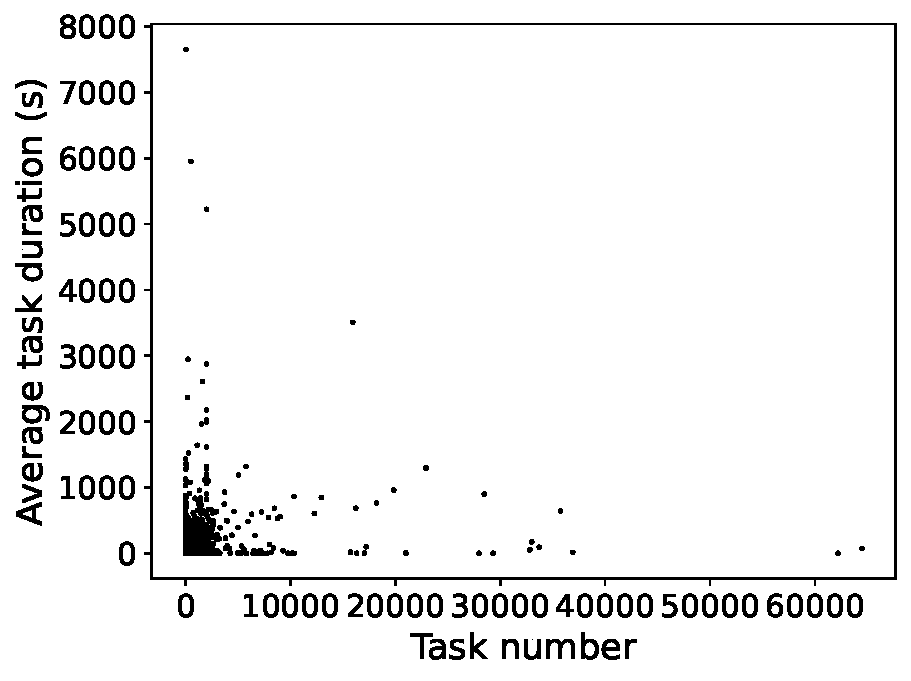
\includegraphics[width=0.47\linewidth]{Image3/JobDistribution_Ali2017_start=0_2D.pdf}%
%\label{fig_second_case}
%\label{Fg:eg1}
}
\hfil
\subfloat[Alibaba 2018]
%
{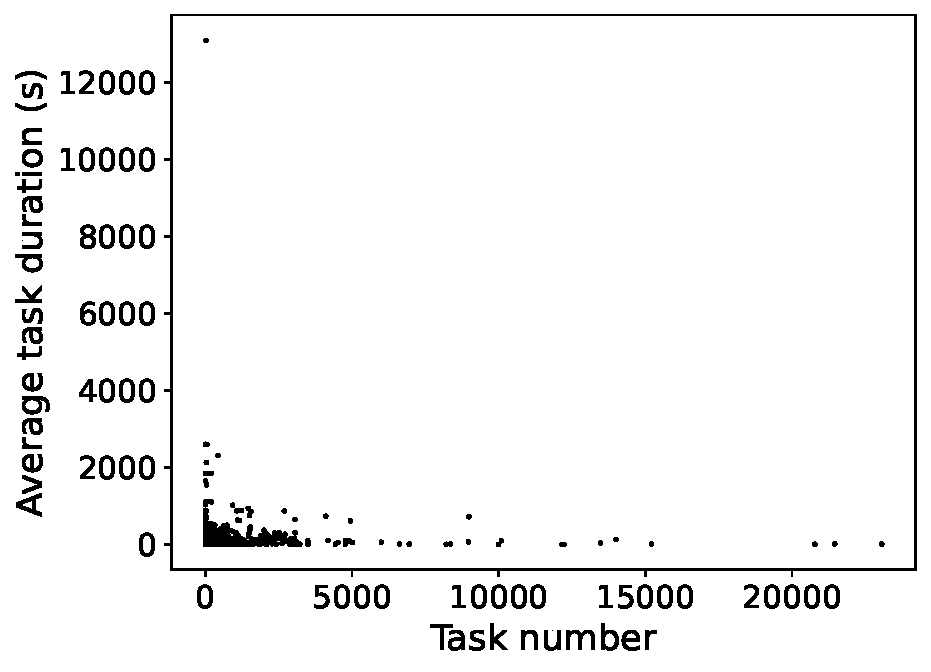
\includegraphics[width=0.48\linewidth]{Image3/JobDistribution_Ali2018_4_start=15000_2D.pdf}%
%\label{Fg:eg2}
}
\caption{Job characteristic distributions of segments sampled from two datasets}
\label{fig:distribution}
\end{figure}
To validate our approach under realistic production conditions, we utilize industrial cluster data from the Alibaba Cluster Trace Program \cite{Ali2017}. We extract essential scheduling telemetry from the raw log files of the 2017 and 2018 releases, capturing the arrival timestamp, task count, and processing duration of each job. From these pre-processed traces, a contiguous segment of 10,000 jobs is randomly sampled from each year to serve as the benchmark driving our simulations. As visualized in Fig. \ref{fig:distribution}, both segments sampled feature a heavy-tailed profile, where a tiny fraction of jobs dominates the vast majority of the total computational demand. Finally, the macro-level characteristics of the segments sampled for experimentation—including mean task counts and average task processing times—are summarized in Table \ref{tab:average_characteristic}.

\begin{table}[t]
    \centering
    \caption{Job characteristics of segments sampled from two datasets}
    \label{tab:average_characteristic}
    \begin{tabular}{ccc}
        \toprule
        Characteristics & Alibaba 2017 & Alibaba 2018 \\
        \midrule
        Average task number per job & $260.11$ & $94.70$ \\
        \midrule
        Average task processing time (s) & $209.18$ & $82.41$ \\
        \bottomrule
    \end{tabular}
\end{table}


\subsection{System Configuration}
We model a distributed environment comprising $m$ identical sites, where each site is provisioned with an equal capacity. To evaluate our algorithms under varying degrees of skewness in workload distribution, we initialize the initial load distribution of each job by deploying its tasks among the sites based on the Zipf distribution and summing up their task processing times at each site. Specifically, the task allocation across sites follows the proportional weights $1, 2^{-\alpha}, 3^{-\alpha}, \dots, m^{-\alpha}$, where the skewness parameter $\alpha$ controls the load imbalance. A higher $\alpha$ value implies that tasks are more heavily concentrated on a small subset of sites, while $\alpha = 0$ indicates a uniform distribution. We evaluate four distinct load distributions by varying $\alpha \in \{0.0, 0.5, 1.0, 2.0\}$. To prevent global load hotspots, we shuffle the order of the sites when deploying each job's task distribution. Additionally, the job arrival times from the trace are linearly scaled to emulate different system utilizations. While we examined various combinations of site numbers, site capacities, and load levels—all yielding consistent performance trends-we focus on presenting the results for a representative setup of $m = 10$ sites, capacity $u=32$ for each site, and $50\%$, $60\%$, $70\%$, and $80\%$ system utilizations.
%We simulate a distributed system of $m$ sites, each with the same number of $32$ computing slots. Each task is assumed to take up one computing slot to run and release it after completion. Due to the switching overhead consideration, we assume that the system does not allow preemption during task execution. For each job, the initial load distribution is generated by randomly deploying its tasks among the sites based on the Zipf distribution and summing up their task processing times: the numbers of tasks placed at the $m$ sites are proportional to $1, \frac{1}{2^\alpha}, \frac{1}{3^\alpha}, ..., \frac{1}{m^\alpha}$, where $\alpha$ is a Zipf parameter. A higher $\alpha$ implies a more skewed distribution (a higher proportion of tasks are concentrated at fewer sites), whereas $\alpha$ = $0$ indicates a uniform distribution. In the experiments, we test four Zipf distributions with $\alpha$ set to $0$, $0.5$, $1$ and $2$ to simulate different task distributions of jobs. After the load distribution is generated, we shuffle the order of the sites when deploying each job's load distribution, so that the total workload at each site will be roughly balanced. We scale the arrival times of the jobs in the datasets to simulate different levels of overall system utilization. We experiment with different numbers of sites, different numbers of computing slots per site, and different levels of system utilization, and the results show similar performance trends. Due to space limitations, we focus on presenting the results for $m=10$ sites, 32 computing slots per site, and system utilization = $50\%$, $60\%$, $70\%$ and $80\%$.


\subsection{Baseline Policies}
We implemented the following baseline policies in the experiments for comparison. The first two baselines are efficiency-targeted policies, namely Shortest Remaining Processing Time (SRPT) and Workload-Aware Greedy Scheduling (SWAG) \cite{hung2015scheduling}. SRPT executes jobs based on their estimated completion time in the case that each job runs alone in the system. In our distributed environment, the estimated completion time of a job $J_i$ is computed as $\max_{j \in[m]} w_{ij}/u_j$ where $w_{ij}$ is the remaining real load of $J_i$ at site $S_j$ and $u_j$ is the capacity of $S_j$. SRPT derives the job execution order by sorting these estimated completion times from low to high. SWAG schedules jobs in a greedy and iterative manner by estimating their completion times based on scheduled workloads in the system. After a job is scheduled, SWAG updates the scheduled workloads at all sites, and estimates the completion times of unscheduled jobs based on the updated workloads. We evaluate PFSP\_SWAG which uses the job execution order derived by SWAG as the hint order $\mathbf{h}$.

In addition, we extend the protective scheduling algorithms in the single-site case (FSP, PFSP and OFSP) to the distributed job execution case based on both of the slack schemes. Under the $IS$ scheme, we have FSP\_i, OFSP\_i and PFSP\_i, which runs FSP, OFSP and PFSP independently at each site. Similarly, under the $GS$ scheme, FSP\_g derives the global job execution order based on the global PS completion times, while OFSP\_g and PFSP\_g prioritize the globally servable or completable job that finishes the fastest if served first, respectively. Since the first job in the global PS order is always servable and completable, OFSP\_g and PFSP\_g are feasible. However, they cannot perfectly guarantee protectiveness, as in the counterexample of Section \ref{sec:conflict}. %For all the policies mentioned, the average time of computing the solution during the simulation is around $10^{-5}$ seconds.

The following example further illustrates how FSP\_g, OFSP\_g and PFSP\_g work in the distributed job execution case. Consider a distributed system of two sites $S_1$ and $S_2$, both with capacity $1$. Suppose at the beginning $t=0$, two jobs $J_1$ and $J_2$ are submitted to the system, with the initial load distribution 
\begin{equation}
    W = \begin{bmatrix} 8 & 9 \\ 10 & 7 \end{bmatrix},
\end{equation}
where $J_1$ has loads $8$ and $9$ on $S_1$ and $S_2$, respectively, and $J_2$ has loads $9$ and $7$ on sites $S_1$ and $S_2$ respectively. The site-specfic PS completion times of the jobs are
\begin{equation}
    \begin{bmatrix} 16 & 16 \\ 18 & 14 \end{bmatrix}.
\end{equation}
Thus, the global PS completion times of $J_1$ and $J_2$ are $16$ and $18$, respectively, and the global PS order is $J_1 \prec J_2$. Therefore, FSP\_g will serve $J_1$ first then $J_2$ at all sites, and the average job response time is $(9+18)/2=13.5$.

We compute the slack system based on the $GS$ scheme: $J_1$ is the first job in the global PS order, so its $GS$ slacks are $[16 - 8=8, 16-9=7]$; $J_2$ is the second job and its $GS$ slacks are $[18 - 10 - 8=0, 18-7-9=2]$, resulting in 
\begin{equation}
    S = \begin{bmatrix} 8 & 7 \\ 0 & 2 \end{bmatrix}
\end{equation}
 In this case, $J_1$ is globally servable and completable, while $J_2$ is not completable because $s_{11} = 8 < w_{21} = 10$. Therefore, PFSP\_g will behave the same as FSP\_g, i.e. serve $J_1$ to completion, and then $J_2$. Meanwhile, $J_2$ is servable since its preceding job $J_1$ has positive slacks $s_{11}=8>0, s_{12}=7>0$ at all sites. $J_2$ will finish at time $t=10$ if it is served first, while $J_1$ will finish at time $t=9$ if it is served first. Therefore, although both jobs are servable, OFSP\_g will also first serve $J_1$ to completion since it finishes earlier than $J_2$, and the average job response time is also $13.5$. 
%In this case, OFSP\_g can serve either of them. Note that if OFSP\_g chooses to serve $J_2$, it can only be served for $7$ seconds because $J_1$'s slack at site $S_2$ decreases to $0$ at $t=7$; After that, OFSP\_g turns to serve $J_1$ instead since $J_1$ becomes the only servable job in the system. When $J_1$ finishes, OFSP\_g turns back to $J_2$ and serve it until $J_2$ finishes. This will result in the average job response time of $(16+17)/2=16.5$.

\subsection{Experimental Results}

\begin{figure*}[t]
    \centering
    \begin{subfigure}[b]{0.4\textwidth}
        \centering
        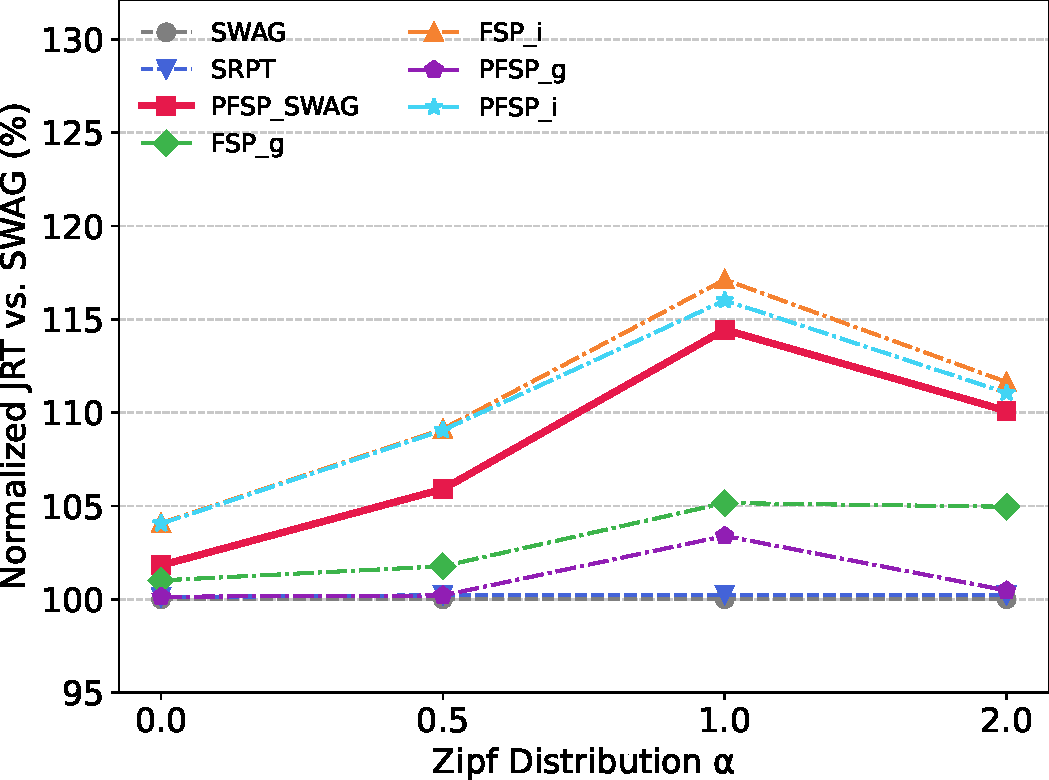
\includegraphics[width=\textwidth]{Image3/Workload_Ali2017_50_Dev=0.0.pdf}
        \caption{Utilization = 50\%}
    \end{subfigure}
    \hfill
    \begin{subfigure}[b]{0.4\textwidth}
        \centering
        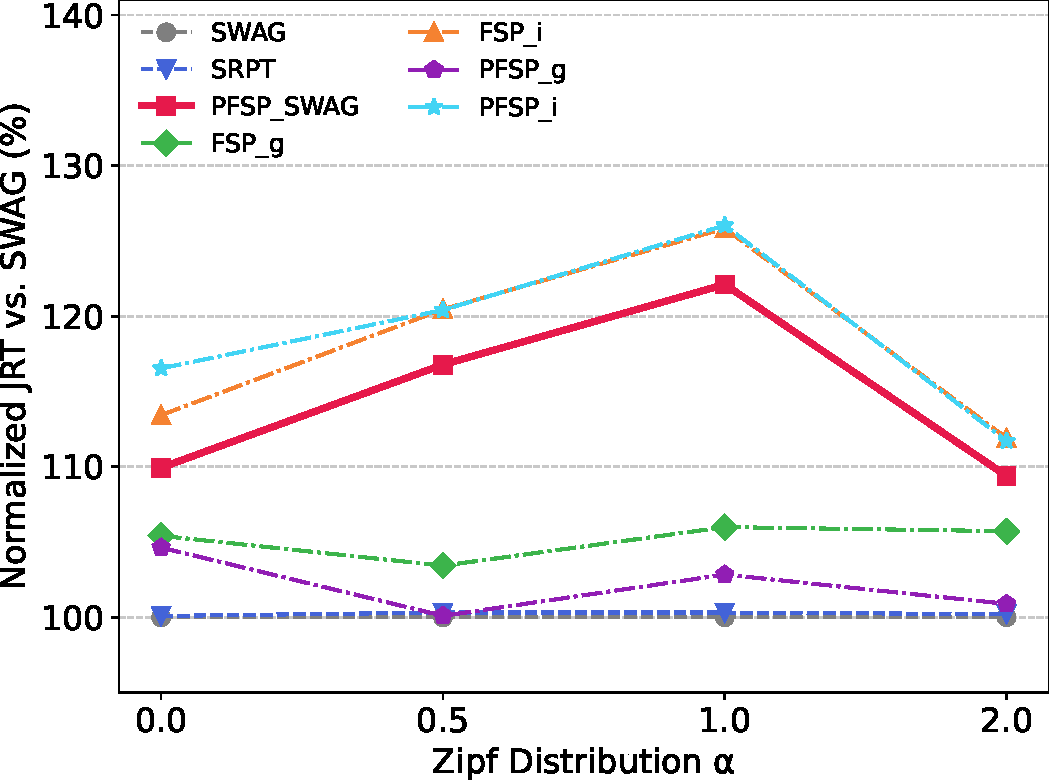
\includegraphics[width=\textwidth]{Image3/Workload_Ali2017_60_Dev=0.0.pdf}
        \caption{Utilization = 60\%}
    \end{subfigure}
    \vspace{0.8em}
    \begin{subfigure}[b]{0.4\textwidth}
        \centering
        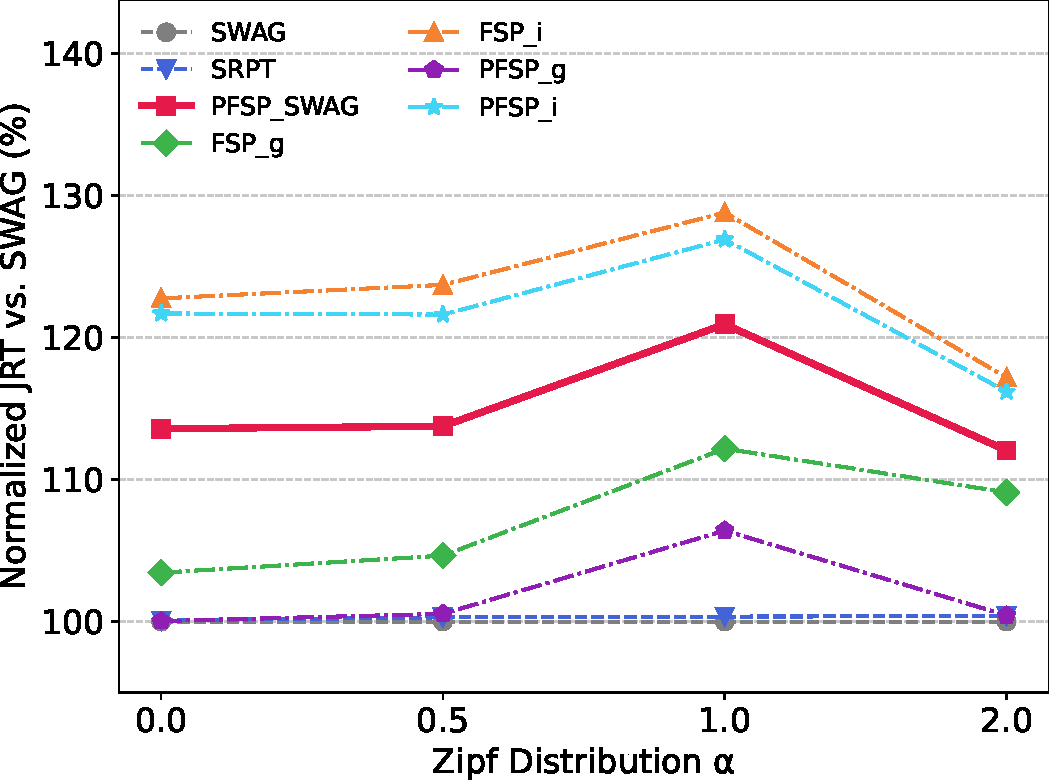
\includegraphics[width=\textwidth]{Image3/Workload_Ali2017_70_Dev=0.0.pdf}
        \caption{Utilization = 70\%}
    \end{subfigure}
    \hfill
    \begin{subfigure}[b]{0.4\textwidth}
        \centering
        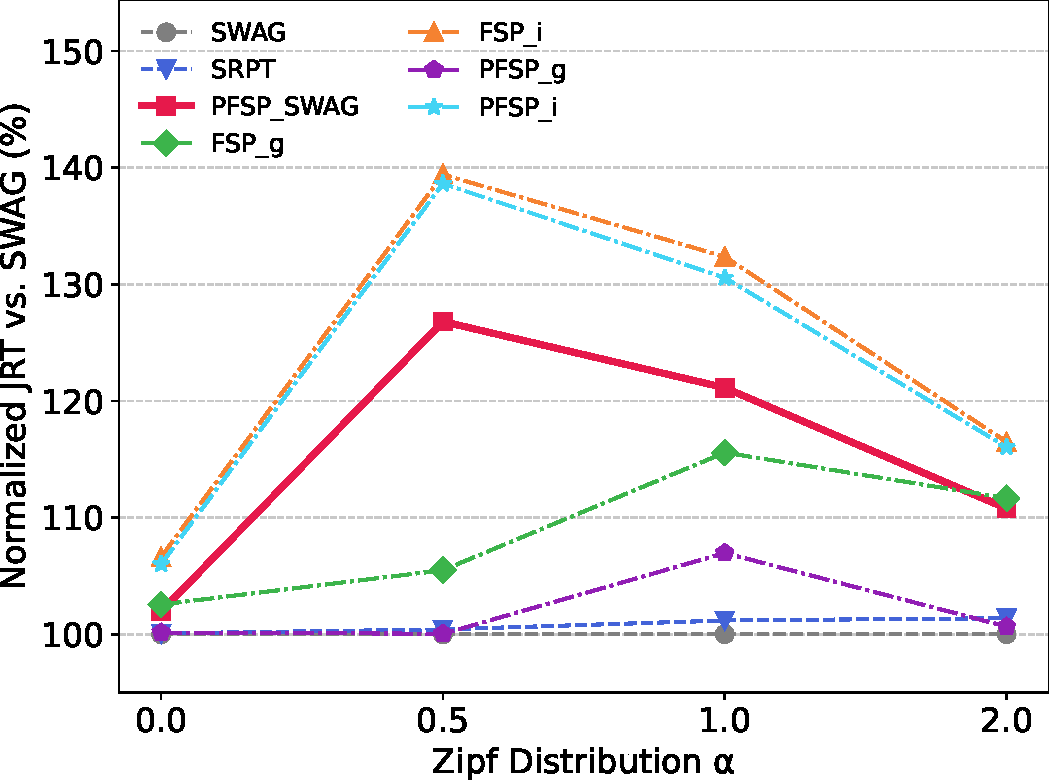
\includegraphics[width=\textwidth]{Image3/Workload_Ali2017_80_Dev=0.0.pdf}
        \caption{Utilization = 80\%}
    \end{subfigure}

    \caption{Average job response time, Alibaba 2017}
    \label{fig:JRT_Ali2017}
\end{figure*}

\begin{figure*}[t]
    \centering
    \begin{subfigure}[b]{0.4\textwidth}
        \centering
        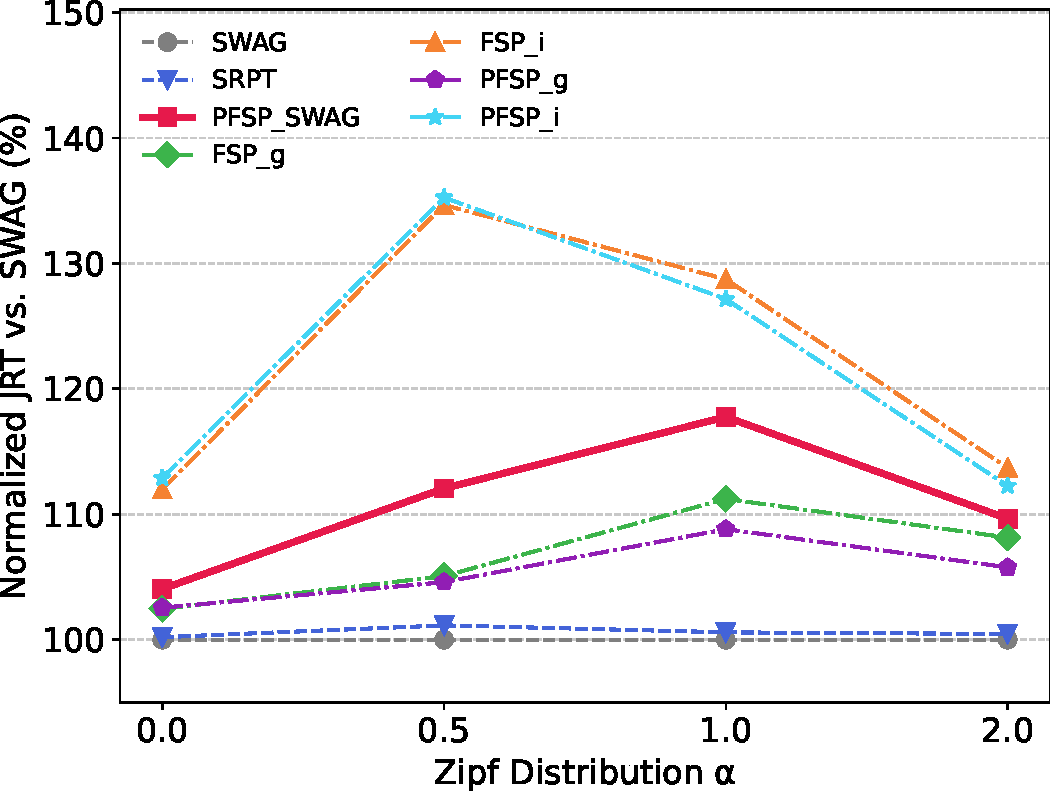
\includegraphics[width=\textwidth]{Image3/Workload_Ali2018_4_50_Dev=0.000.pdf}
        \caption{Utilization = 50\%}
    \end{subfigure}
    \hfill
    \begin{subfigure}[b]{0.4\textwidth}
        \centering
        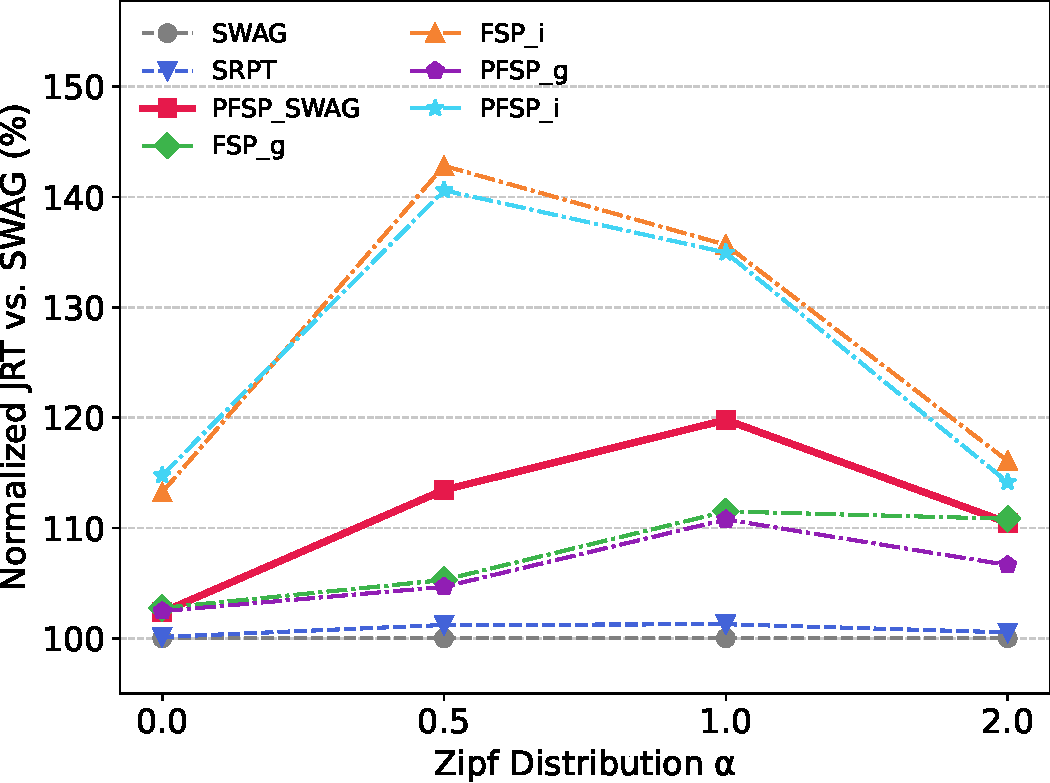
\includegraphics[width=\textwidth]{Image3/Workload_Ali2018_4_60_Dev=0.000.pdf}
        \caption{Utilization = 60\%}
    \end{subfigure}
    \vspace{0.8em}
    \begin{subfigure}[b]{0.4\textwidth}
        \centering
        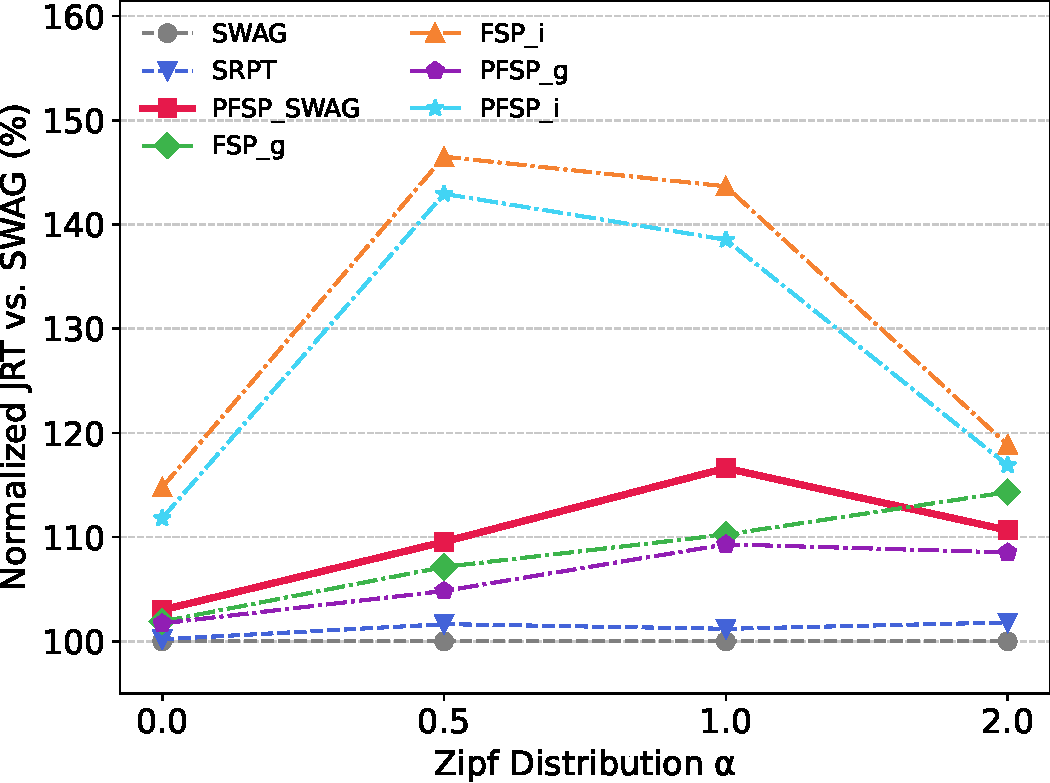
\includegraphics[width=\textwidth]{Image3/Workload_Ali2018_4_70_Dev=0.000.pdf}
        \caption{Utilization = 70\%}
    \end{subfigure}
    \hfill
    \begin{subfigure}[b]{0.4\textwidth}
        \centering
        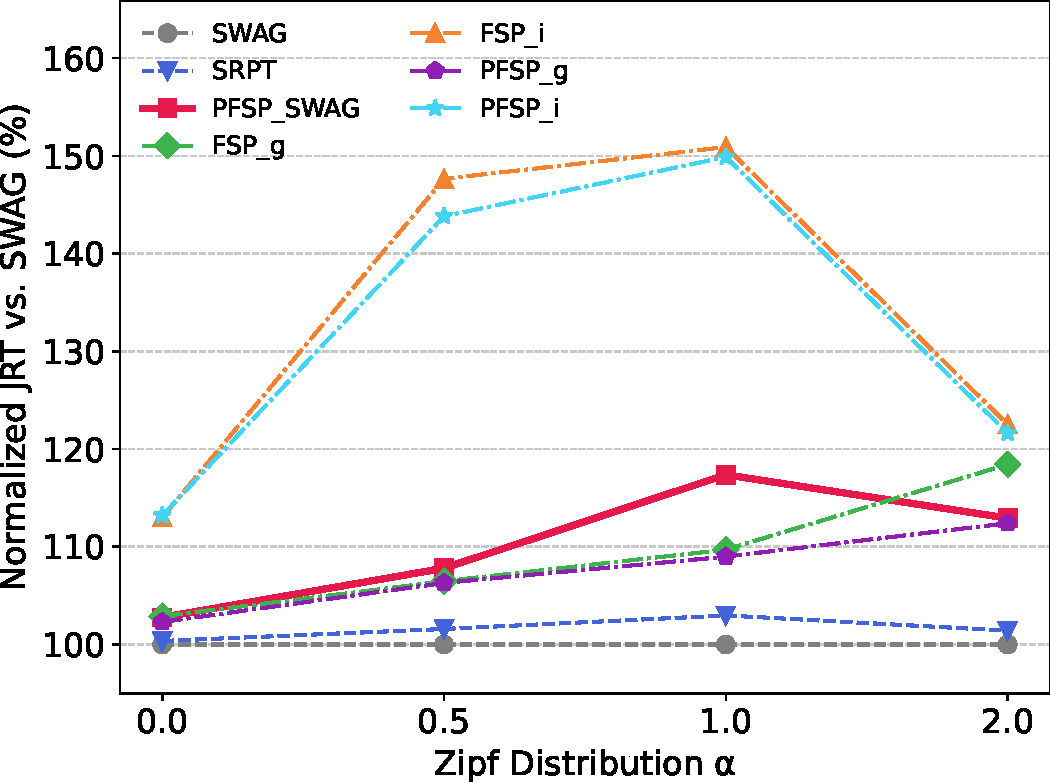
\includegraphics[width=\textwidth]{Image3/Workload_Ali2018_4_80_Dev=0.000.pdf}
        \caption{Utilization = 80\%}
    \end{subfigure}

    \caption{Average job response time, Alibaba 2018}
    \label{fig:JRT_Ali2018}
\end{figure*}

We use the average job response time and the number of jobs violating PS deadlines as the performance metrics to evaluate the dual objectives of efficiency and fairness under different scheduling policies, system utilizations and load distributions. The average job response time is defined as the average time span from each job's arrival to its completion, where a lower average job response time indicates higher job processing efficiency of the policy. The number of jobs violating PS deadlines is defined as the number of jobs whose actual completion time are later than their global PS completion times, which indicates the degree of long-term fairness in the system. A larger number of violations means that more jobs fail to finish before their completion times under the distributed PS policy, indicating a higher degree of unfairness/starvation in job scheduling. Because some of the policies have similar performance trends, we only present the results of SWAG, SRPT (efficiency-targeted policies), PFSP\_g, FSP\_g (policies based on the $GS$ scheme), PFSP\_i, FSP\_i (policies based on the $IS$ scheme) and PFSP\_SWAG (derived from the PFSP\_x framework).

Figures \ref{fig:JRT_Ali2017} and \ref{fig:JRT_Ali2018} present the average job response time of different scheduling policies under various system settings. To facilitate comparison, we set the optimal average job response time derived from SWAG policy as the $100\%$ baseline and compute the average job response time of other policies as a percentage of it. The results demonstrate that scheduling policies that are efficiency-targeted (SWAG and SRPT) or adopt the $GS$ scheme (PFSP\_g, FSP\_g) achieve better average job response times compared to those adopting the $IS$ scheme. In particular, PFSP\_g achieves fairly close performance to the SWAG policy, demonstrating its potential in balancing the trade-off between efficiency and long-term fairness. In contrast, policies that adopt the $IS$ scheme (PFSP\_i, FSP\_i, PFSP\_SWAG) guarantee strict protectiveness at the expense of worse average job response times, with the performance gap reaching up to approximately 50\%. Our proposed PFSP\_SWAG algorithm demonstrates the best average job response time among the three policies based on the $IS$ scheme, and under certain system configurations when the load distributions of jobs are highly skewed (i.e., $\alpha=2.0$), it can even outperforms the FSP\_g policy based on the $GS$ scheme.

\begin{table}[htbp]
    \centering
    \caption{Number of jobs violating PS deadlines, Alibaba 2017}
    \label{tab:count_PS_violation_Ali2017}
    \begin{tabular}{cc cccc}
        \toprule
        \multirow{2}{*}{Utilization} & \multirow{2}{*}{$\alpha$} & \multicolumn{4}{c}{Strategies} \\
        \cmidrule(lr){3-6}
        & & SWAG & SRPT & PFSP\_g & FSP\_g \\
        \midrule
        \multirow{4}{*}{$50\%$} 
        & $0.0$ & 44 & 50 & 0 & 0 \\
        & $0.5$ & 50 & 68 & 0 & 0 \\
        & $1.0$ & 50 & 68 & 0 & 0 \\
        & $2.0$ & 37 & 53 & 0 & 0 \\
        \midrule
        \multirow{4}{*}{$60\%$} 
        & $0.0$ & 41 & 46 & 0 & 0 \\
        & $0.5$ & 43 & 57 & 1 & 0 \\
        & $1.0$ & 34 & 46 & 0 & 0 \\
        & $2.0$ & 25 & 31 & 0 & 0 \\
        \midrule
        \multirow{4}{*}{$70\%$} 
        & $0.0$ & 36 & 41 & 0 & 0 \\
        & $0.5$ & 33 & 40 & 2 & 2 \\
        & $1.0$ & 23 & 28 & 0 & 0 \\
        & $2.0$ & 14 & 21 & 1 & 0 \\
        \midrule
        \multirow{4}{*}{$80\%$} 
        & $0.0$ & 29 & 32 & 1 & 1 \\
        & $0.5$ & 20 & 19 & 0 & 0 \\
        & $1.0$ & 15 & 20 & 0 & 0 \\
        & $2.0$ & 12 & 22 & 0 & 0 \\
        \bottomrule
    \end{tabular}
\end{table}

\begin{table}[htbp]
    \centering
    \caption{Number of jobs violating PS deadlines, Alibaba 2018}
    \label{tab:count_PS_violation_Ali2018}
    \begin{tabular}{cc cccc}
        \toprule
        \multirow{2}{*}{Utilization} & \multirow{2}{*}{$\alpha$} & \multicolumn{4}{c}{Strategies} \\
        \cmidrule(lr){3-6}
        & & SWAG & SRPT & PFSP\_g & FSP\_g \\
        \midrule
        \multirow{4}{*}{$50\%$} 
        & $0.0$ & 37 & 50 & 0 & 0 \\
        & $0.5$ & 57 & 64 & 1 & 0 \\
        & $1.0$ & 41 & 47 & 0 & 0 \\
        & $2.0$ & 23 & 36 & 0 & 0 \\
        \midrule
        \multirow{4}{*}{$60\%$} 
        & $0.0$ & 26 & 38 & 1 & 1 \\
        & $0.5$ & 40 & 46 & 0 & 0 \\
        & $1.0$ & 28 & 28 & 0 & 0 \\
        & $2.0$ & 17 & 26 & 0 & 0 \\
        \midrule
        \multirow{4}{*}{$70\%$} 
        & $0.0$ & 17 & 31 & 2 & 2 \\
        & $0.5$ & 32 & 41 & 0 & 0 \\
        & $1.0$ & 23 & 25 & 0 & 0 \\
        & $2.0$ & 14 & 23 & 0 & 0 \\
        \midrule
        \multirow{4}{*}{$80\%$} 
        & $0.0$ & 13 & 25 & 1 & 1 \\
        & $0.5$ & 32 & 41 & 0 & 0 \\
        & $1.0$ & 18 & 18 & 0 & 0 \\
        & $2.0$ & 12 & 18 & 0 & 0 \\
        \bottomrule
    \end{tabular}
\end{table}

Tables \ref{tab:count_PS_violation_Ali2017} and \ref{tab:count_PS_violation_Ali2018} present the number of violations to the PS deadline under different scheduling policies. We omit the $IS$ policies (including PFSP\_SWAG) from the tables because they guarantee zero violations under all conditions. The results show that both SWAG and SRPT have tens of violations in general, indicating that efficiency-targeted policies do not guarantee protectiveness in the distributed job execution case. In contrast, policies based on the $GS$ scheme have much fewer violations (zero violations in most cases). In particulr, PFSP\_g significantly decreases the number of violations while keeping a close average job response time to SWAG and SRPT at all system settings, demonstrating that it achieves a good trade-off between efficiency and long-term fairness. Meanwhile, PFSP\_SWAG guarantees zero violations while effectively decreasing the average job response time compared to other policies based on the $IS$ scheme. These empirical results suggest that the PFSP\_g and PFSP\_SWAG can be selectively applied to different scenarios depending on the system's specific trade-offs between fairness and efficiency.

\subsection{On Inaccurate Job Load Estimation}

All scheduling policies introduced above rely on accurate estimations of job load distributions across sites. Inaccurate estimations can lead to system performance degradation in both average job response time and PS deadline violations. To evaluate the impact of inaccurate estimations, we randomly generate the job load estimates following a uniform distribution between $-x$ and $x$, where $x$ is the maximum deviation assumed. Based on our evaluation with 10,000 jobs, when the estimated job loads uniformly deviate within $\pm10\%$ of the ground truth (i.e., ranging from $90\%$ to $110\%$), the number of jobs violating PS deadlines rises up to hundreds across different scheduling policies. Estimation errors manifest in two distinct forms:

\begin{itemize}[leftmargin=*]
    \item \textbf{Over-estimation} gives a larger estimated load of a job than its actual load, which may deprioritize it in the execution order. In this case, other jobs in the system can either have their execution order advanced or kept unchanged, so generally their completion times will not degrade and the number of jobs violating PS deadlines will increase by one at most. Consequently, over-estimation predominantly impacts the over-estimated job itself, degrading its own completion time.%  potentially leading to earlier completion times.    However, because other concurrently running jobs will either have higher priorities or keep the priorities unchanged, their completion times generally remain within their PS deadlines. 
    
    \item \textbf{Under-estimation} gives a smaller estimated load of a job than its actual load. As a result, an under-estimated job is not completed and needs to continue execution even when its (estimated) real load drops to 0. This introduces severe systemic risks because with its (estimated) real load being 0, it will be prioritized for execution by all scheduling policies (including efficiency-targeted ones and those based on the GS and IS schemes), inducing serious head-of-line blocking and starving subsequent jobs, which ultimately triggers a surge of PS deadline violations.
\end{itemize}

To counteract performance degradation under job load under-estimations, we propose a mitigation mechanism, called Processor Sharing Fallback (PSF). PSF allocates a fair capacity share to these under-estimated jobs: Once a job has its (estimated) real load drop to 0 at a site but has not completed execution at this site, it transitions into a fallback PS state. In this state, the job is assigned a fixed equal share ($1/N_{\text{active}}$) of the site capacity, where $N_{\text{active}}$ represents the concurrent count of active jobs with remaining real load at the site. The leftover capacity of the site is then used to schedule non-fallback jobs following the original scheduling policy. Note that the PSF mechanism will be activated only when a job's load is underestimated. Consequently, it can be seamlessly integrated as a lightweight add-on module to existing scheduling policies, incurring negligible overhead when load estimations are accurate.%Note that the PSF mechanism will only be triggered if a job has its load under-estimated, thus it can be deployed as an add-on mechanism with little overhead when the system has accurate load estimation.
%This indicates that the PSF mechanism effectively mitigates the performance degradation caused by under-estimation of job loads. %The results show that the PSF mechanism effectively mitigates the performance degradation caused by under-estimation of job loads, especially for efficiency-targeted policies (SWAG and SRPT) and policies based on the $GS$ scheme (PFSP\_g and FSP\_g). With the PSF mechanism, these policies can achieve average job response times close to their counterparts with accurate job load estimations, while significantly reducing the number of PS deadline violations.


\begin{table}[ht]
\centering
\caption{Number of jobs violating PS deadlines with/without PSF, 10\% deviation, 70\% utilization, Alibaba 2017}
\label{tab:PSF_ali17_1}
\resizebox{\textwidth}{!}{\begin{tabular}{l cccc c cccc}
\toprule
& \multicolumn{4}{c}{\textbf{Without PSF}} & & \multicolumn{4}{c}{\textbf{With PSF}} \\
\cmidrule{2-5} \cmidrule{7-10}
\textbf{Policy} & $\alpha=0.0$ & $\alpha=0.5$ & $\alpha=1.0$ & $\alpha=2.0$ & & $\alpha=0.0$ & $\alpha=0.5$ & $\alpha=1.0$ & $\alpha=2.0$ \\
\midrule
SWAG & 173  & 300 & 357 & 732 & & 69 & 91 & 97 & 160 \\
SRPT & 182 & 322 & 369 & 768 & & 82 & 102 & 102 & 164 \\
PFSP\_g & 217 & 195 & 363 & 577 & & 48 & 52 & 57 & 109 \\
FSP\_g & 104 & 83 & 79 & 52 & & 29 & 48 & 53 & 110 \\
PFSP\_SWAG & 543 & 973 & 909 & 888 & & 70 & 74 & 65 & 72 \\
PFSP\_i & 774 & 1232 & 978 & 981 & &  79 & 80 & 62 & 72 \\
FSP\_i & 285 & 547 & 513 & 480 & & 71 & 71 & 58 & 67 \\
\bottomrule
\end{tabular}}
\end{table}

\begin{table}[ht]
\centering
\caption{Number of jobs violating PS deadlines with/without PSF, 20\% deviation, 70\% utilization, Alibaba 2017}
\label{tab:PSF_ali17_2}
\resizebox{\textwidth}{!}{
\begin{tabular}{l cccc c cccc}
\toprule
& \multicolumn{4}{c}{\textbf{Without PSF}} & & \multicolumn{4}{c}{\textbf{With PSF}} \\
\cmidrule{2-5} \cmidrule{7-10}
\textbf{Policy} & $\alpha=0.0$ & $\alpha=0.5$ & $\alpha=1.0$ & $\alpha=2.0$ & & $\alpha=0.0$ & $\alpha=0.5$ & $\alpha=1.0$ & $\alpha=2.0$ \\
\midrule
SWAG & 443  & 366 & 556 & 1185 & & 97 & 135 & 136 & 214 \\
SRPT & 451 & 372 & 552 & 1149 & & 108 & 133 & 135 & 226 \\
PFSP\_g & 395 & 371 & 521 & 791 & & 80 & 113 & 110 & 172 \\
FSP\_g & 245 & 167 & 197 & 184 & & 78 & 106 & 105 & 167 \\
PFSP\_SWAG & 970 & 1509 & 1606 & 1519 & & 97 & 143 & 98 & 107 \\
PFSP\_i & 1314 & 1976 & 1623 & 1662 & & 109 & 147 & 102 & 106 \\
FSP\_i & 439 & 920 & 1039 & 1000 & & 98 & 147 & 98 & 94 \\
\bottomrule
\end{tabular}}
\end{table}

\begin{table}[ht]
\centering
\caption{Number of jobs violating PS deadlines with/without PSF, 30\% deviation, 70\% utilization, Alibaba 2017}
\label{tab:PSF_ali17_3}
\resizebox{\textwidth}{!}{
\begin{tabular}{l cccc c cccc}
\toprule
& \multicolumn{4}{c}{\textbf{Without PSF}} & & \multicolumn{4}{c}{\textbf{With PSF}} \\
\cmidrule{2-5} \cmidrule{7-10}
\textbf{Policy} & $\alpha=0.0$ & $\alpha=0.5$ & $\alpha=1.0$ & $\alpha=2.0$ & & $\alpha=0.0$ & $\alpha=0.5$ & $\alpha=1.0$ & $\alpha=2.0$ \\
\midrule
SWAG & 369  & 607 & 896 & 1495 & & 106 & 146 & 178 & 184 \\
SRPT & 363 & 666 & 889 & 1526 & & 108 & 143 & 780 & 182 \\
PFSP\_g & 317 & 561 & 580 & 1476 & & 84 & 105 & 118 & 162 \\
FSP\_g & 132 & 191 & 169 & 547 & & 84 & 98 & 112 & 161 \\
PFSP\_SWAG & 632 & 1499 & 1486 & 2157 & & 114 & 130 & 134 & 154 \\
PFSP\_i & 697 & 1721 & 1466 & 2421 & &  125 & 136 & 126 & 146 \\
FSP\_i & 293 & 872 & 740 & 1465 & & 116 & 131 & 120 & 142 \\
\bottomrule
\end{tabular}}
\end{table}

\begin{table}[ht]
\centering
\caption{Number of jobs violating PS deadlines with/without PSF, 40\% deviation, 70\% utilization, Alibaba 2017}
\label{tab:PSF_ali17_4}
\resizebox{\textwidth}{!}{
\begin{tabular}{l cccc c cccc}
\toprule
& \multicolumn{4}{c}{\textbf{Without PSF}} & & \multicolumn{4}{c}{\textbf{With PSF}} \\
\cmidrule{2-5} \cmidrule{7-10}
\textbf{Policy} & $\alpha=0.0$ & $\alpha=0.5$ & $\alpha=1.0$ & $\alpha=2.0$ & & $\alpha=0.0$ & $\alpha=0.5$ & $\alpha=1.0$ & $\alpha=2.0$ \\
\midrule
SWAG & 1143  & 1351 & 1925 & 2826 & & 140 & 282 & 306 & 352 \\
SRPT & 1147 & 1518 & 1920 & 2819 & & 141 & 260 & 327 & 326 \\
PFSP\_g & 1060 & 1304 & 1488 & 2631 & & 120 & 245 & 215 & 296 \\
FSP\_g & 354 & 548 & 597 & 1572 & & 111 & 248 & 205 & 301 \\
PFSP\_SWAG & 1640 & 2353 & 3338 & 3375 & & 149 & 199 & 215 & 247 \\
PFSP\_i & 1903 & 2911 & 3648 & 3765 & &  159 & 205 & 237 & 248 \\
FSP\_i & 748 & 1438 & 2391 & 2582 & & 144 & 199 & 222 & 249 \\
\bottomrule
\end{tabular}}
\end{table}

\begin{table}[ht]
\centering
\caption{Number of jobs violating PS deadlines with/without PSF, 10\% deviation, 70\% utilization, Alibaba 2018}
\label{tab:PSF_ali18_1}
\resizebox{\textwidth}{!}{\begin{tabular}{l cccc c cccc}
\toprule
& \multicolumn{4}{c}{\textbf{Without PSF}} & & \multicolumn{4}{c}{\textbf{With PSF}} \\
\cmidrule{2-5} \cmidrule{7-10}
\textbf{Policy} & $\alpha=0.0$ & $\alpha=0.5$ & $\alpha=1.0$ & $\alpha=2.0$ & & $\alpha=0.0$ & $\alpha=0.5$ & $\alpha=1.0$ & $\alpha=2.0$ \\
\midrule
SWAG & 92  & 98 & 188 & 178 & & 44 & 47 & 62 & 76 \\
SRPT & 108 & 91 & 200 & 183 & & 55 & 52 & 69 & 81 \\
PFSP\_g & 81 & 40 & 133 & 149 & & 30 & 19 & 27 & 62 \\
FSP\_g & 53 & 27 & 37 & 30 & & 29 & 20 & 25 & 65 \\
PFSP\_SWAG & 394 & 247 & 461 & 276 & & 39 & 41 & 31 & 37 \\
PFSP\_i & 423 & 350 & 513 & 307 & &  41 & 37 & 37 & 42 \\
FSP\_i & 196 & 102 & 258 & 137 & & 36 & 34 & 31 & 36 \\
\bottomrule
\end{tabular}}
\end{table}

\begin{table}[ht]
\centering
\caption{Number of jobs violating PS deadlines with/without PSF, 20\% deviation, 70\% utilization, Alibaba 2018}
\label{tab:PSF_ali18_2}
\resizebox{\textwidth}{!}{
\begin{tabular}{l cccc c cccc}
\toprule
& \multicolumn{4}{c}{\textbf{Without PSF}} & & \multicolumn{4}{c}{\textbf{With PSF}} \\
\cmidrule{2-5} \cmidrule{7-10}
\textbf{Policy} & $\alpha=0.0$ & $\alpha=0.5$ & $\alpha=1.0$ & $\alpha=2.0$ & & $\alpha=0.0$ & $\alpha=0.5$ & $\alpha=1.0$ & $\alpha=2.0$ \\
\midrule
SWAG & 145  & 209 & 425 & 398 & & 38 & 63 & 65 & 90 \\
SRPT & 163 & 209 & 394 & 408 & & 48 & 64 & 67 & 84 \\
PFSP\_g & 144 & 216 & 315 & 346 & & 34 & 33 & 45 & 70 \\
FSP\_g & 70 & 52 & 99 & 94 & & 33 & 32 & 44 & 73 \\
PFSP\_SWAG & 450 & 564 & 745 & 541 & & 45 & 55 & 53 & 51 \\
PFSP\_i & 498 & 625 & 774 & 536 & &  46 & 58 & 51 & 49 \\
FSP\_i & 185 & 293 & 355 & 281 & & 44 & 53 & 50 & 48 \\
\bottomrule
\end{tabular}}
\end{table}

\begin{table}[ht]
\centering
\caption{Number of jobs violating PS deadlines with/without PSF, 30\% deviation, 70\% utilization, Alibaba 2018}
\label{tab:PSF_ali18_3}
\resizebox{\textwidth}{!}{
\begin{tabular}{l cccc c cccc}
\toprule
& \multicolumn{4}{c}{\textbf{Without PSF}} & & \multicolumn{4}{c}{\textbf{With PSF}} \\
\cmidrule{2-5} \cmidrule{7-10}
\textbf{Policy} & $\alpha=0.0$ & $\alpha=0.5$ & $\alpha=1.0$ & $\alpha=2.0$ & & $\alpha=0.0$ & $\alpha=0.5$ & $\alpha=1.0$ & $\alpha=2.0$ \\
\midrule
SWAG & 880  & 386 & 801 & 746 & & 106 & 80 & 161 & 176 \\
SRPT & 884 & 362 & 761 & 760 & & 113 & 88 & 150 & 180 \\
PFSP\_g & 947 & 290 & 597 & 638 & & 101 & 59 & 156 & 156 \\
FSP\_g & 243 & 87 & 89 & 218 & & 99 & 56 & 153 & 165 \\
PFSP\_SWAG & 1666 & 1078 & 1785 & 946 & & 135 & 75 & 121 & 88 \\
PFSP\_i & 2009 & 1426 & 2012 & 1103 & &  140 & 80 & 131 & 93 \\
FSP\_i & 767 & 423 & 935 & 514 & & 143 & 71 & 126 & 88 \\
\bottomrule
\end{tabular}}
\end{table}

\begin{table}[ht]
\centering
\caption{Number of jobs violating PS deadlines with/without PSF, 40\% deviation, 70\% utilization, Alibaba 2018}
\label{tab:PSF_ali18_4}
\resizebox{\textwidth}{!}{
\begin{tabular}{l cccc c cccc}
\toprule
& \multicolumn{4}{c}{\textbf{Without PSF}} & & \multicolumn{4}{c}{\textbf{With PSF}} \\
\cmidrule{2-5} \cmidrule{7-10}
\textbf{Policy} & $\alpha=0.0$ & $\alpha=0.5$ & $\alpha=1.0$ & $\alpha=2.0$ & & $\alpha=0.0$ & $\alpha=0.5$ & $\alpha=1.0$ & $\alpha=2.0$ \\
\midrule
SWAG & 778  & 369 & 927 & 779 & & 134 & 123 & 199 & 151 \\
SRPT & 801 & 408 & 964 & 751 & & 142 & 127 & 198 & 152 \\
PFSP\_g & 727 & 327 & 817 & 624 & & 126 & 95 & 176 & 130 \\
FSP\_g & 446 & 191 & 386 & 263 & & 123 & 95 & 177 & 139 \\
PFSP\_SWAG & 1229 & 903 & 2053 & 940 & & 178 & 124 & 167 & 106 \\
PFSP\_i & 1325 & 1074 & 2085 & 980 & &  173 & 133 & 171 & 107 \\
FSP\_i & 779 & 507 & 1452 & 419 & & 170 & 129 & 166 & 110 \\
\bottomrule
\end{tabular}}
\end{table}


Tables \ref{tab:PSF_ali17_1} through \ref{tab:PSF_ali18_4} illustrate the impact of the PSF mechanism on PS deadline violations under different deviations of job load estimations (maximum deviation = $10\%$, $20\%$, $30\%$ and $40\%$) for both datasets. Since the performance trends for different system utilizations are similar, we present the representative results for $70\%$ system utilization only.  As can be seen, integrating the PSF mechanism significantly reduces violations for all policies, where our proposed protective scheduling policies outperform efficiency-targeted baselines in most cases, especially when the job load distributions are highly skewed. It can also be observed that policies based on the GS scheme (FSP\_g, PFSP\_g) yield the lowest violation counts. This is because these policies set the global PS completion time of a job as its deadline at all sites for scheduling purposes. The global PS completion time is given by the maximum of the site-specific PS completion times across all sites. Thus, it is less affected by under-estimation of job loads at individual sites than the site-specific PS completion times. %The results indicate that policies under the $GS$ scheme (FSP\_g, PFSP\_g) inherently yield the lowest violation counts.



\begin{figure*}[t]
    \centering
    \begin{subfigure}[b]{0.4\textwidth}
        \centering
        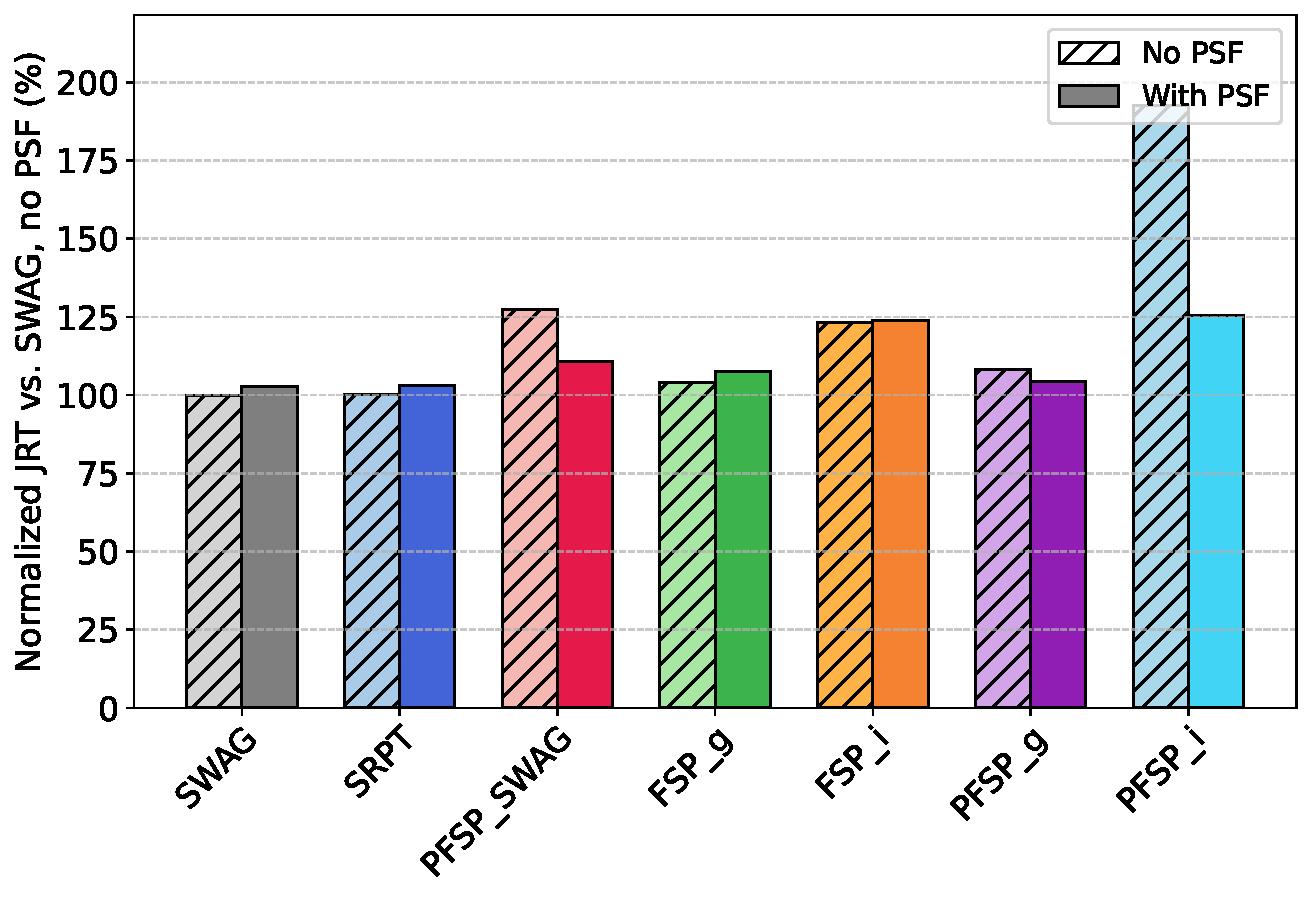
\includegraphics[width=\textwidth]{Image3/PSF_Bar_Ali2017_70_alpha=0.0_dev=0.1.pdf}
        \caption{$\alpha = 0.0$}
    \end{subfigure}
    \hfill
    \begin{subfigure}[b]{0.4\textwidth}
        \centering
        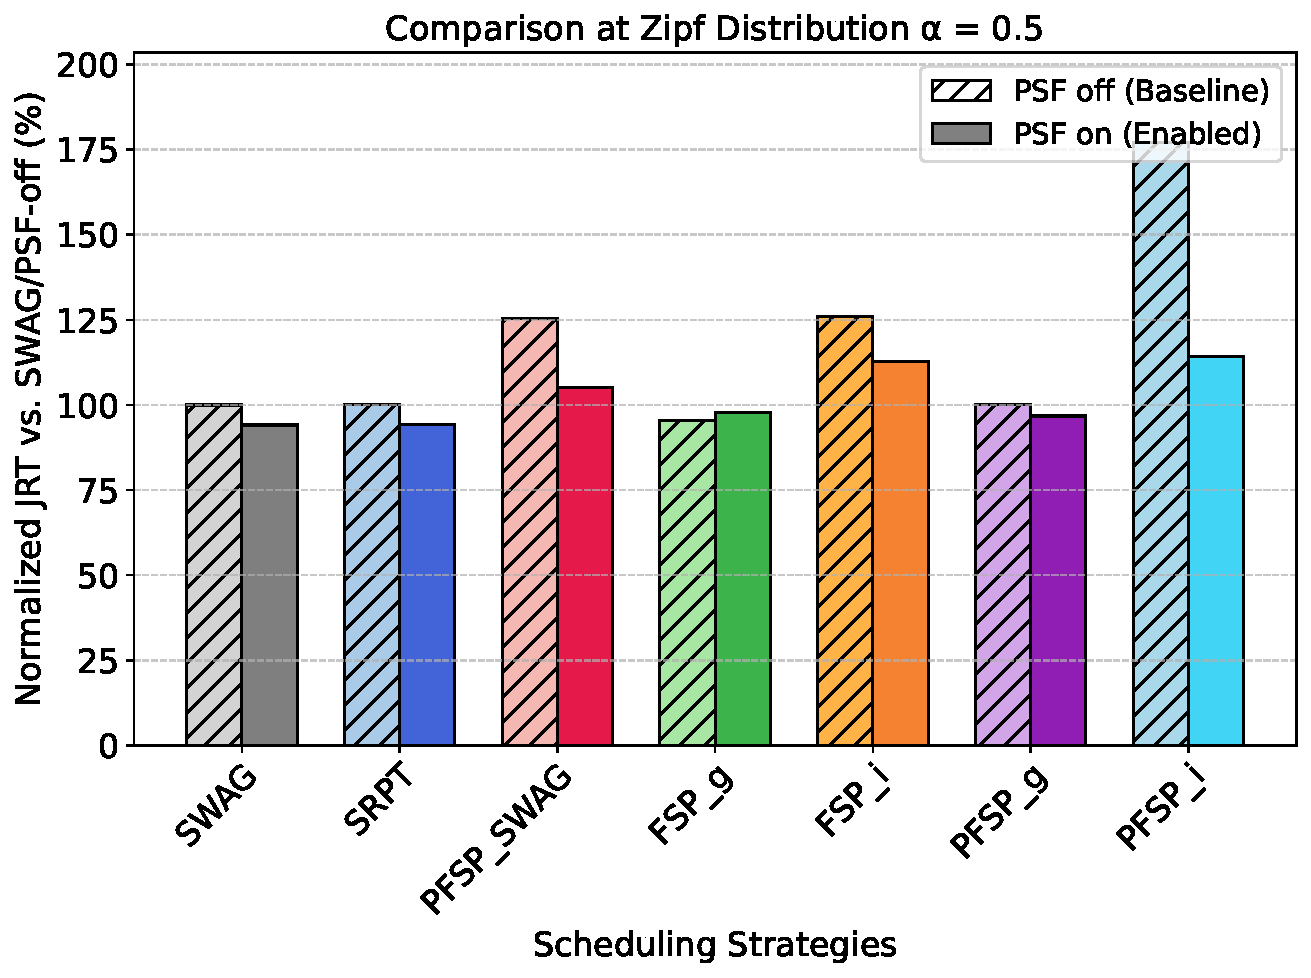
\includegraphics[width=\textwidth]{Image3/PSF_Bar_Ali2017_70_alpha=0.5_dev=0.1.pdf}
        \caption{$\alpha = 0.5$}
    \end{subfigure}
    \vspace{0.8em}
    \begin{subfigure}[b]{0.4\textwidth}
        \centering
        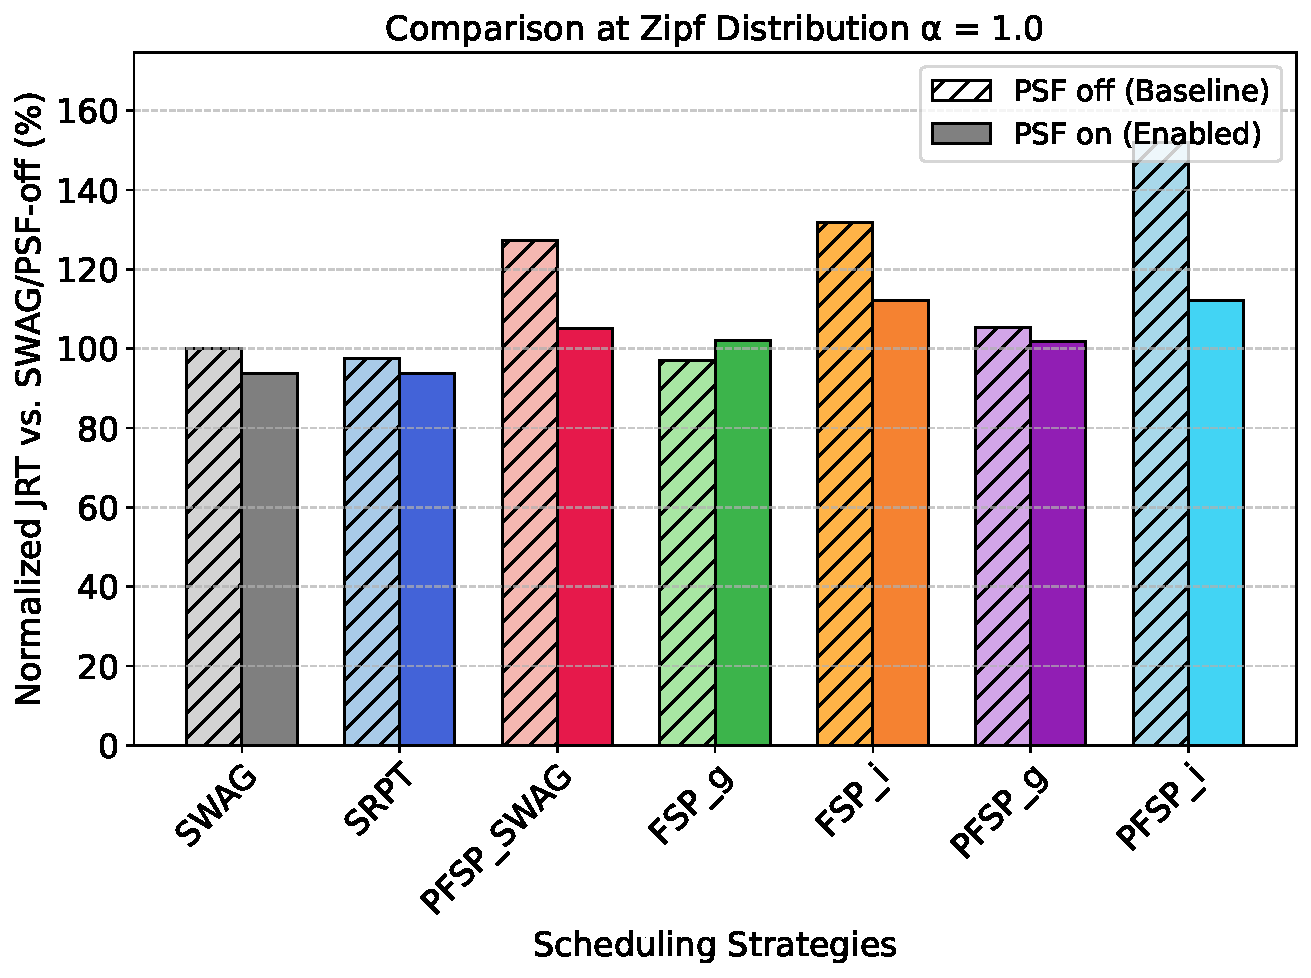
\includegraphics[width=\textwidth]{Image3/PSF_Bar_Ali2017_70_alpha=1.0_dev=0.1.pdf}
        \caption{$\alpha = 1.0$}
    \end{subfigure}
    \hfill
    \begin{subfigure}[b]{0.4\textwidth}
        \centering
        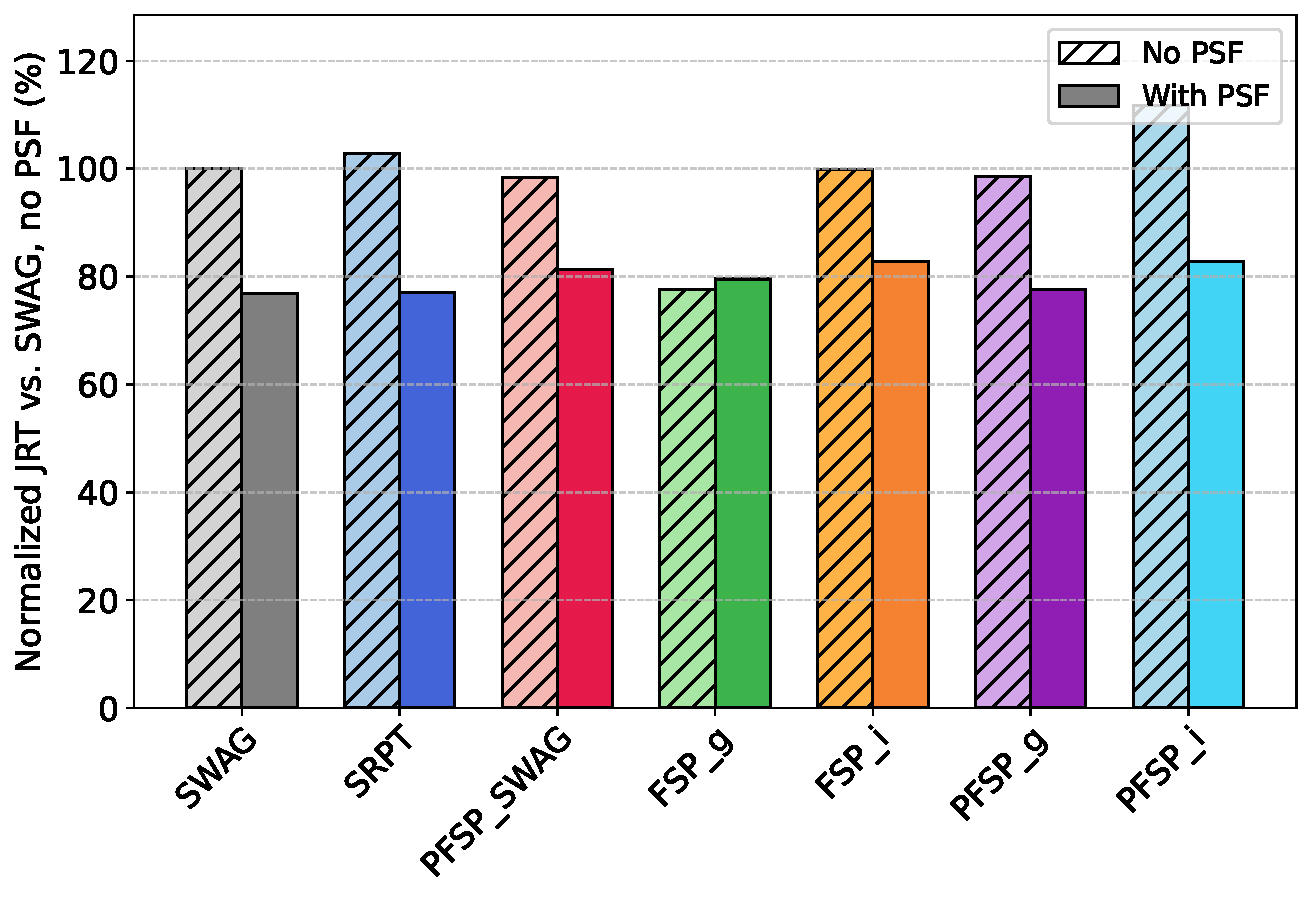
\includegraphics[width=\textwidth]{Image3/PSF_Bar_Ali2017_70_alpha=2.0_dev=0.1.pdf}
        \caption{$\alpha = 2.0$}
    \end{subfigure}

    \caption{Average job response time with/without PSF, 10\% deviation, 70\% utilization, Alibaba 2017}
    \label{fig:JRT_Ali2017_err=0.1}
\end{figure*}

\begin{figure*}[t]
    \centering
    \begin{subfigure}[b]{0.4\textwidth}
        \centering
        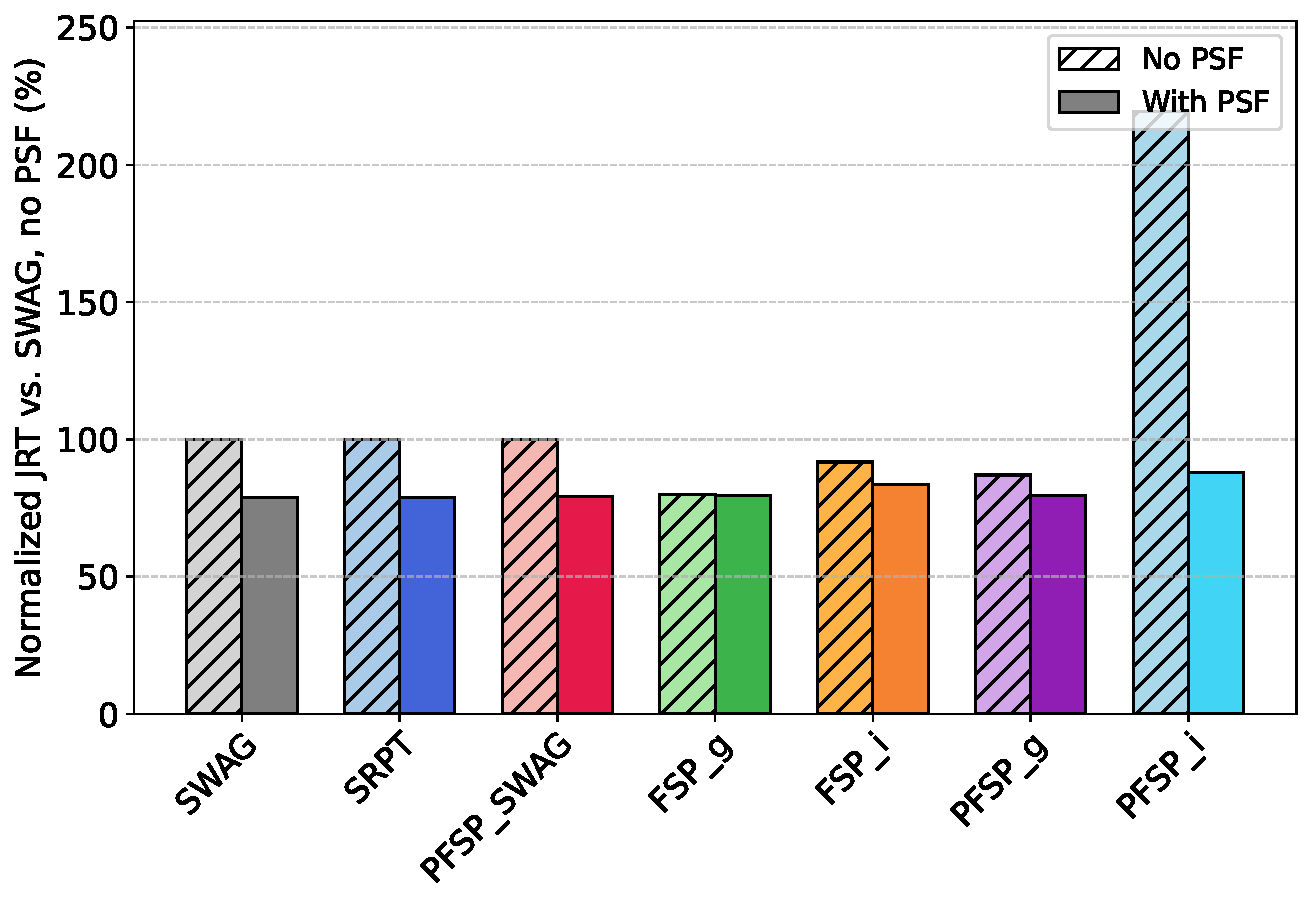
\includegraphics[width=\textwidth]{Image3/PSF_Bar_Ali2017_70_alpha=0.0_dev=0.2.pdf}
        \caption{$\alpha = 0.0$}
    \end{subfigure}
    \hfill
    \begin{subfigure}[b]{0.4\textwidth}
        \centering
        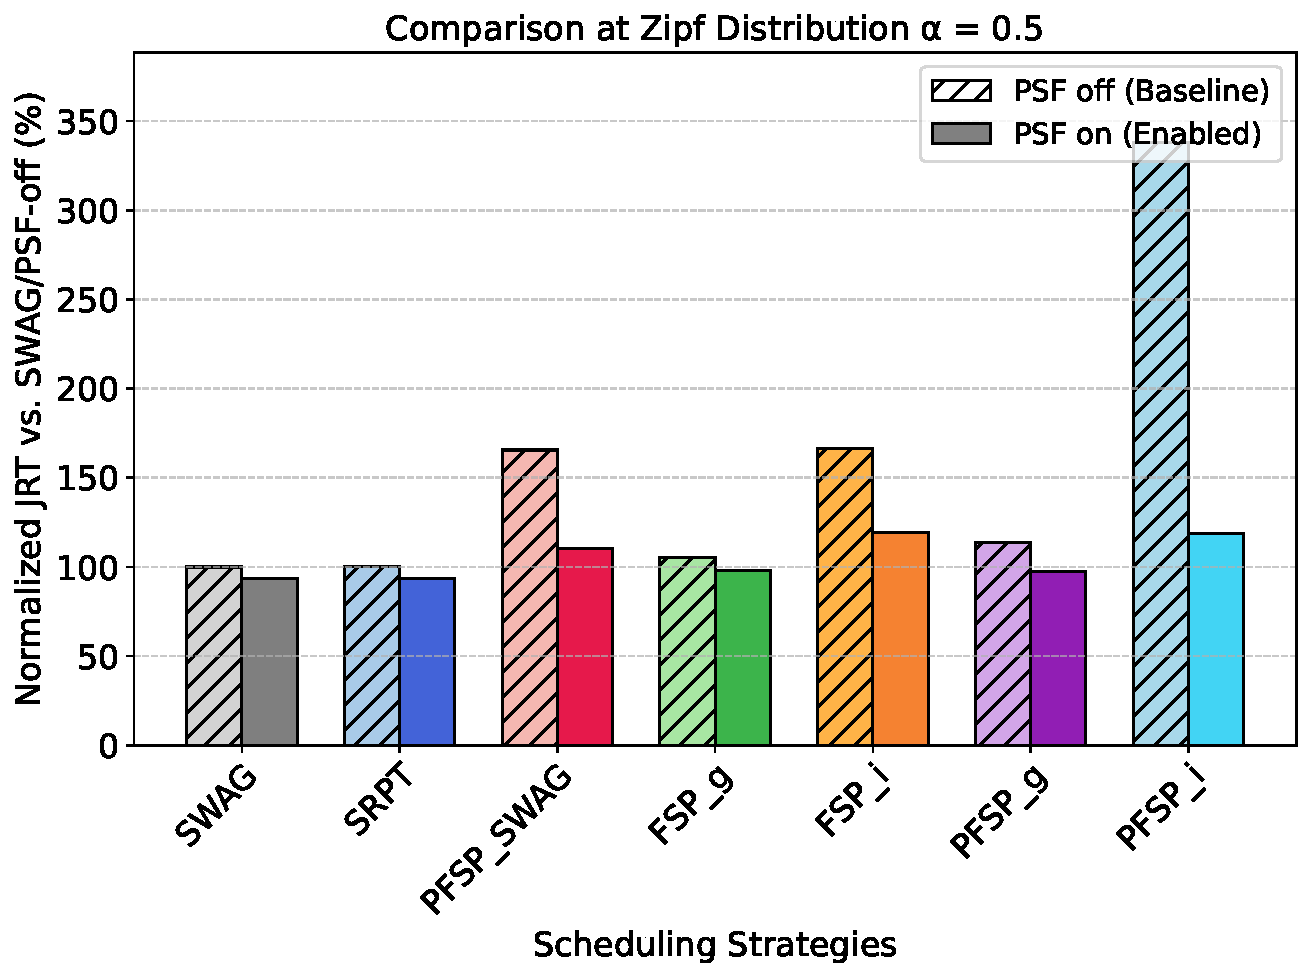
\includegraphics[width=\textwidth]{Image3/PSF_Bar_Ali2017_70_alpha=0.5_dev=0.2.pdf}
        \caption{$\alpha = 0.5$}
    \end{subfigure}
    \vspace{0.8em}
    \begin{subfigure}[b]{0.4\textwidth}
        \centering
        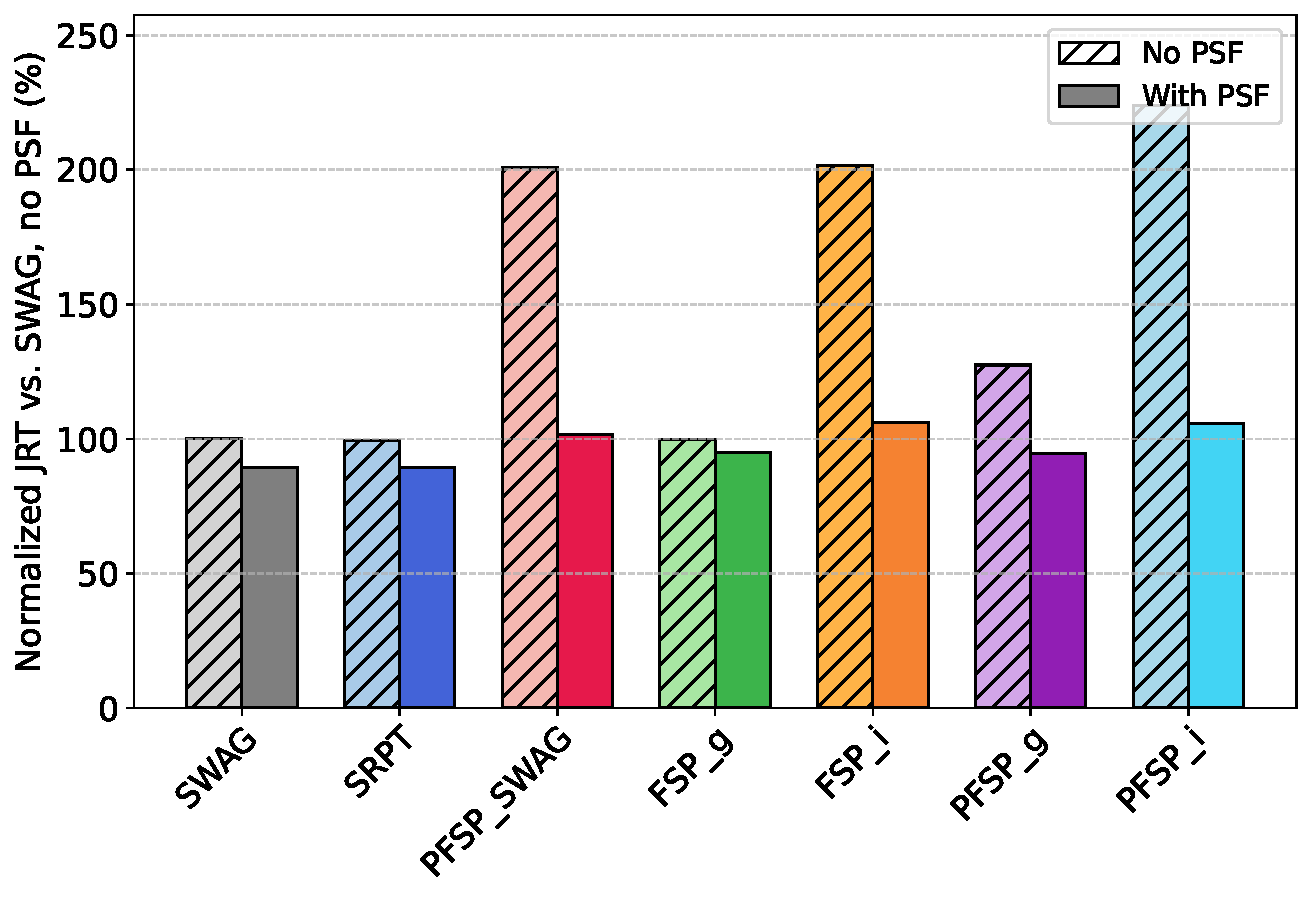
\includegraphics[width=\textwidth]{Image3/PSF_Bar_Ali2017_70_alpha=1.0_dev=0.2.pdf}
        \caption{$\alpha = 1.0$}
    \end{subfigure}
    \hfill
    \begin{subfigure}[b]{0.4\textwidth}
        \centering
        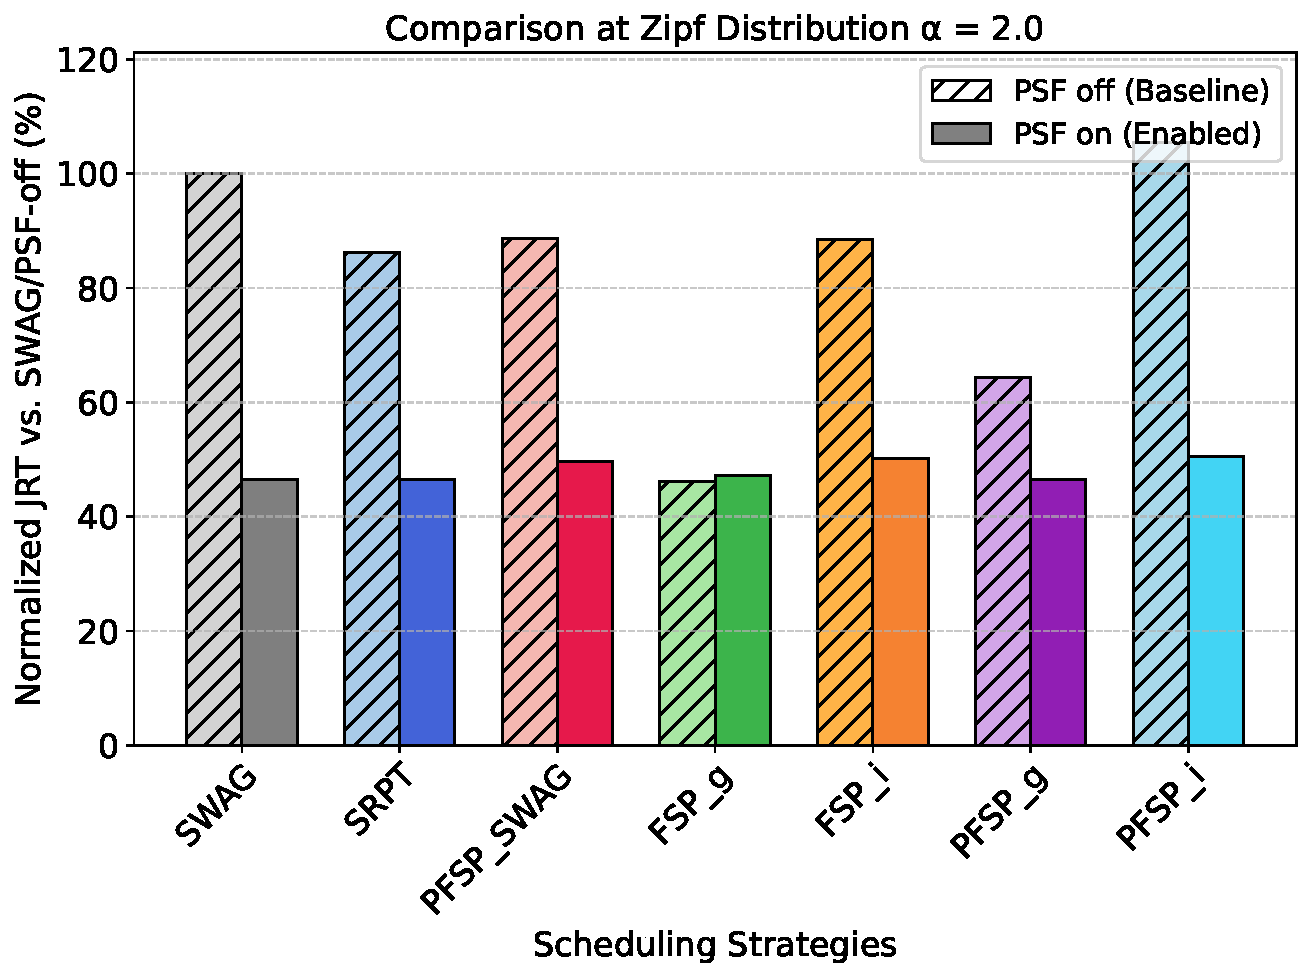
\includegraphics[width=\textwidth]{Image3/PSF_Bar_Ali2017_70_alpha=2.0_dev=0.2.pdf}
        \caption{$\alpha = 2.0$}
    \end{subfigure}

    \caption{Average job response time with/without PSF, 20\% deviation, 70\% utilization, Alibaba 2017}
    \label{fig:JRT_Ali2017_err=0.2}
\end{figure*}

\begin{figure*}[t]
    \centering
    \begin{subfigure}[b]{0.4\textwidth}
        \centering
        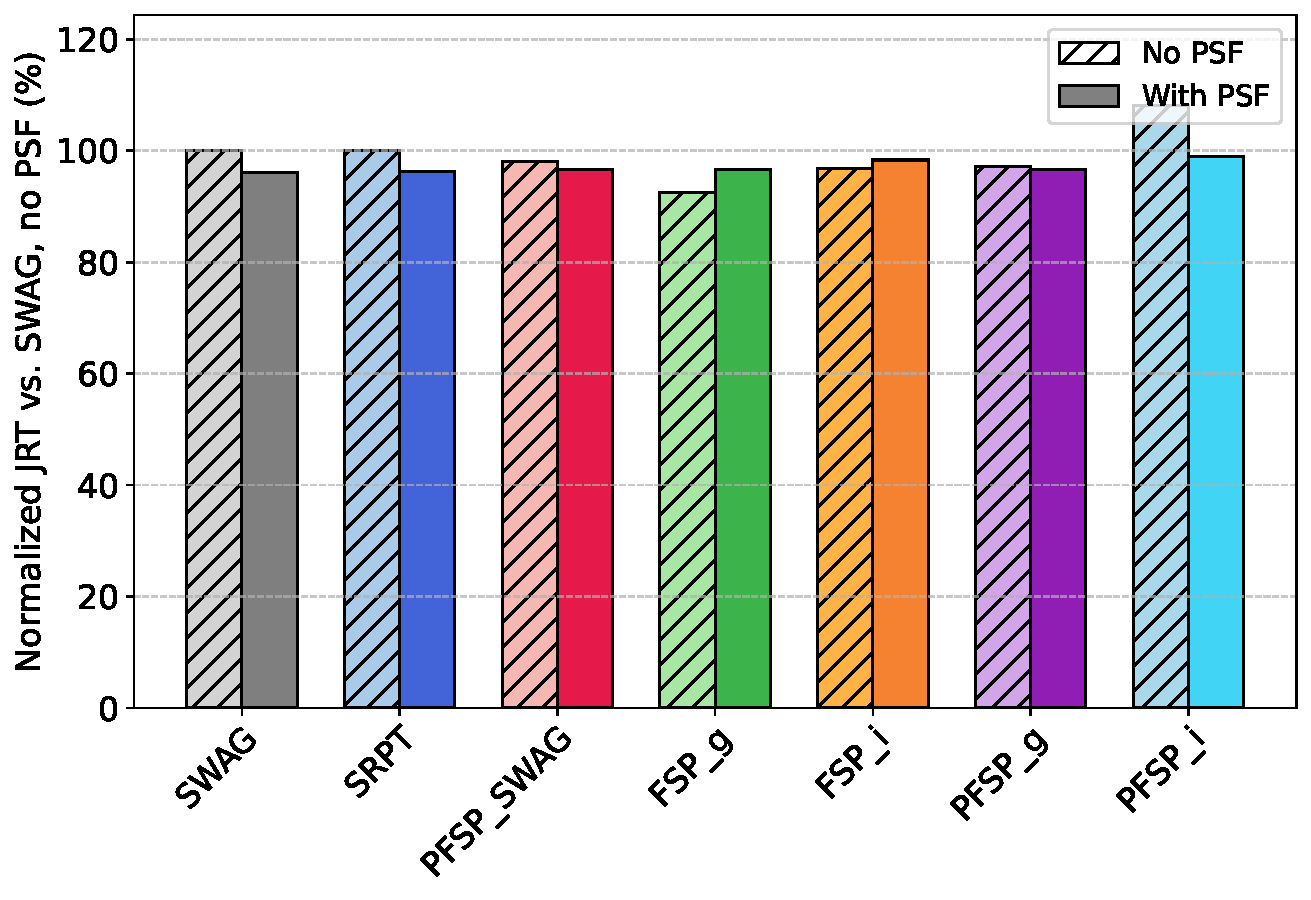
\includegraphics[width=\textwidth]{Image3/PSF_Bar_Ali2017_70_alpha=0.0_dev=0.3.pdf}
        \caption{$\alpha = 0.0$}
    \end{subfigure}
    \hfill
    \begin{subfigure}[b]{0.4\textwidth}
        \centering
        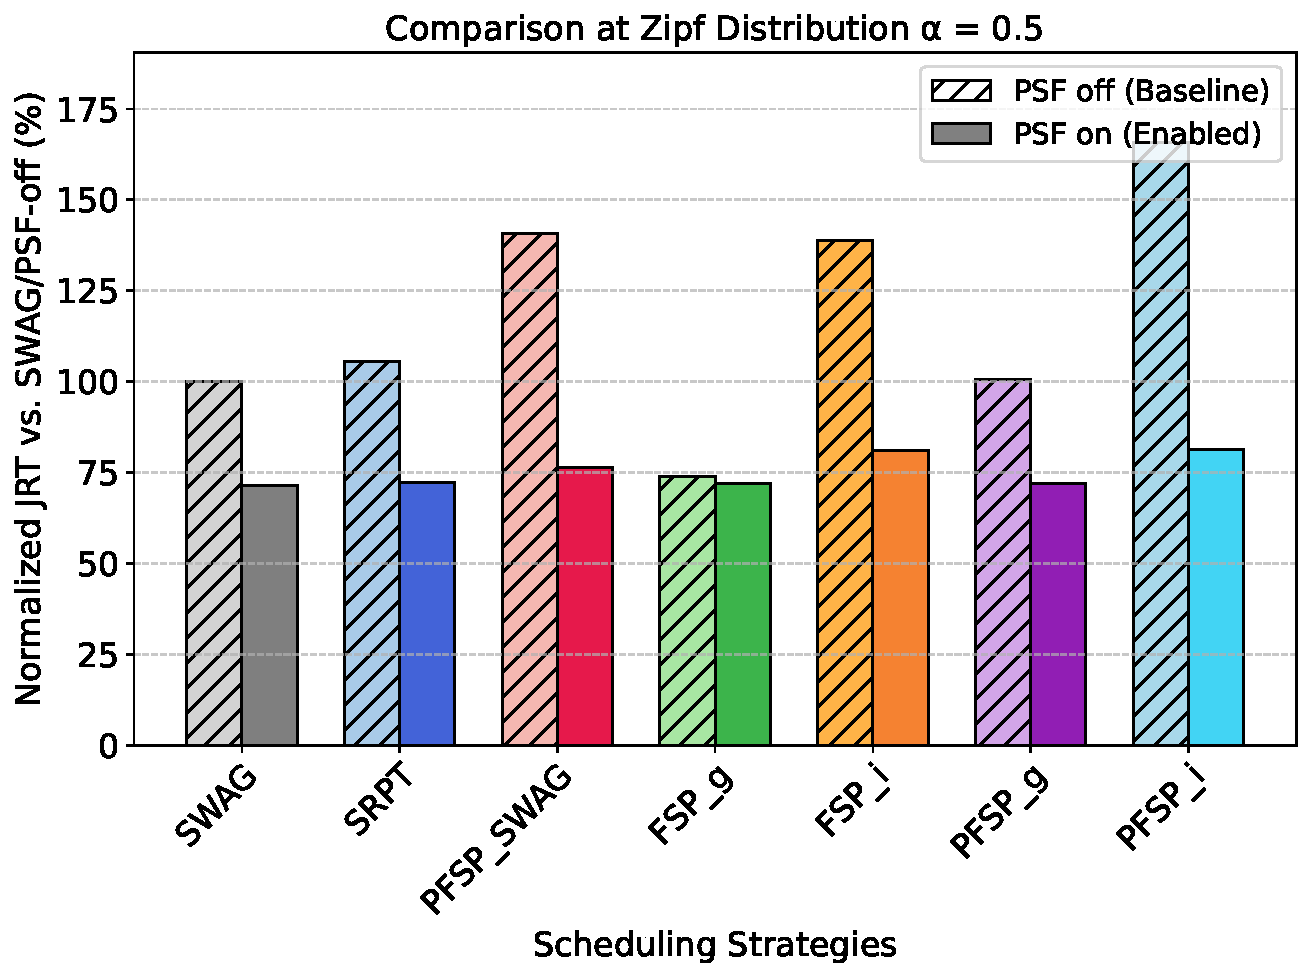
\includegraphics[width=\textwidth]{Image3/PSF_Bar_Ali2017_70_alpha=0.5_dev=0.3.pdf}
        \caption{$\alpha = 0.5$}
    \end{subfigure}
    \vspace{0.8em}
    \begin{subfigure}[b]{0.4\textwidth}
        \centering
        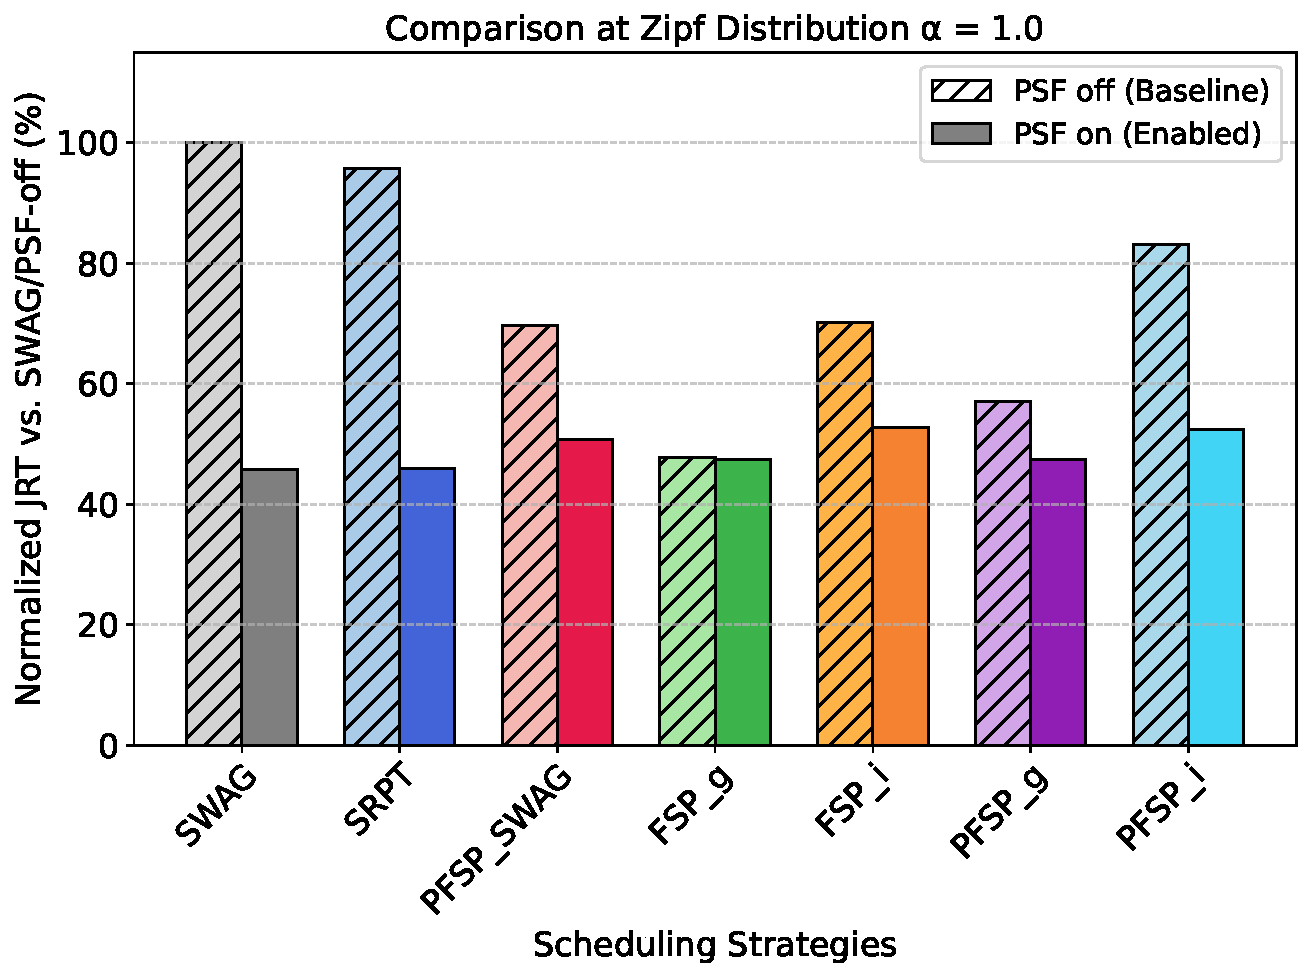
\includegraphics[width=\textwidth]{Image3/PSF_Bar_Ali2017_70_alpha=1.0_dev=0.3.pdf}
        \caption{$\alpha = 1.0$}
    \end{subfigure}
    \hfill
    \begin{subfigure}[b]{0.4\textwidth}
        \centering
        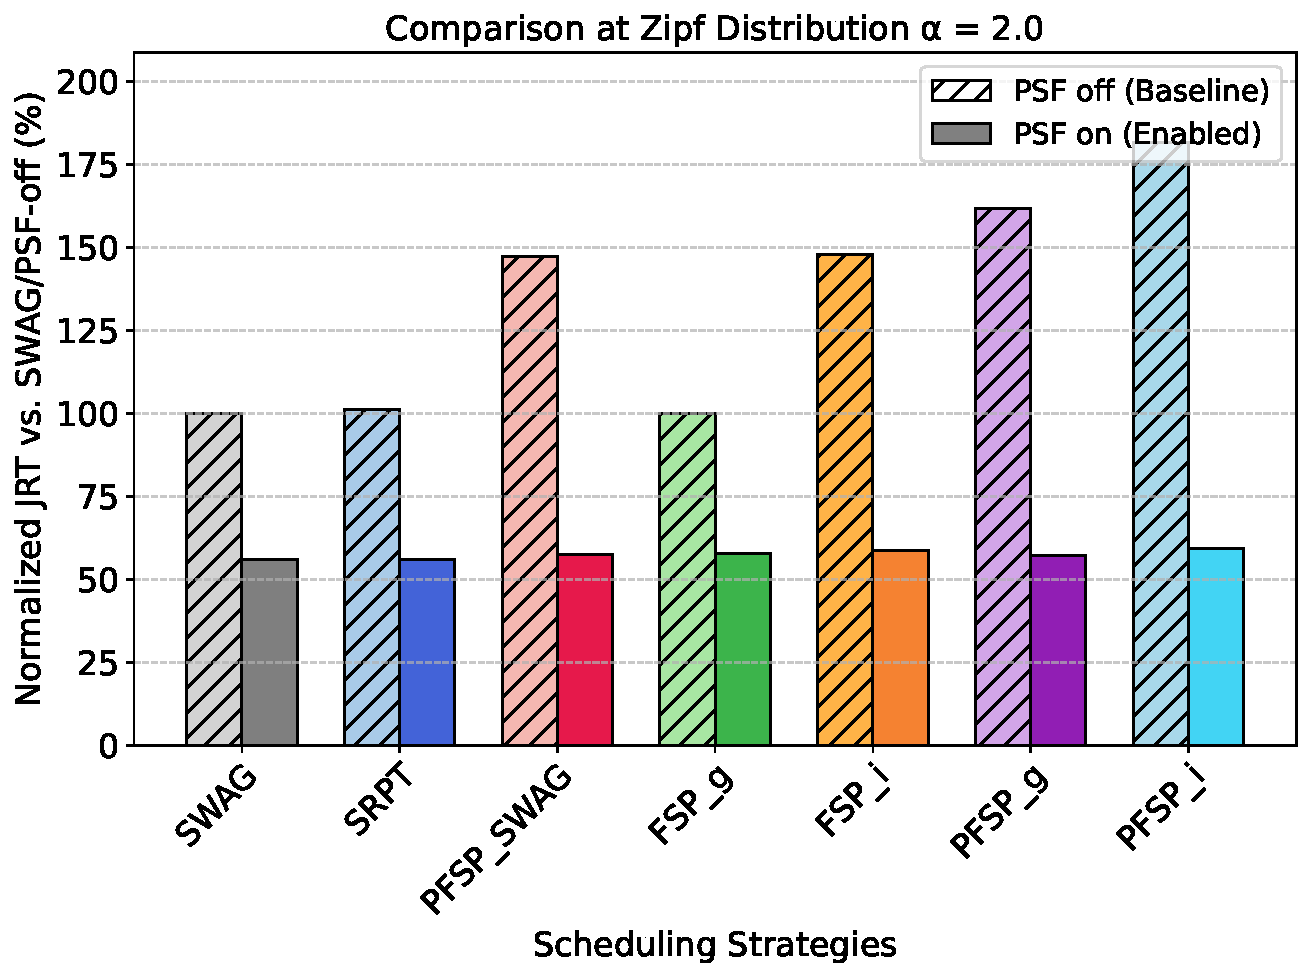
\includegraphics[width=\textwidth]{Image3/PSF_Bar_Ali2017_70_alpha=2.0_dev=0.3.pdf}
        \caption{$\alpha = 2.0$}
    \end{subfigure}

    \caption{Average job response time with/without PSF, 30\% deviation, 70\% utilization, Alibaba 2017}
    \label{fig:JRT_Ali2017_err=0.3}
\end{figure*}

\begin{figure*}[t]
    \centering
    \begin{subfigure}[b]{0.4\textwidth}
        \centering
        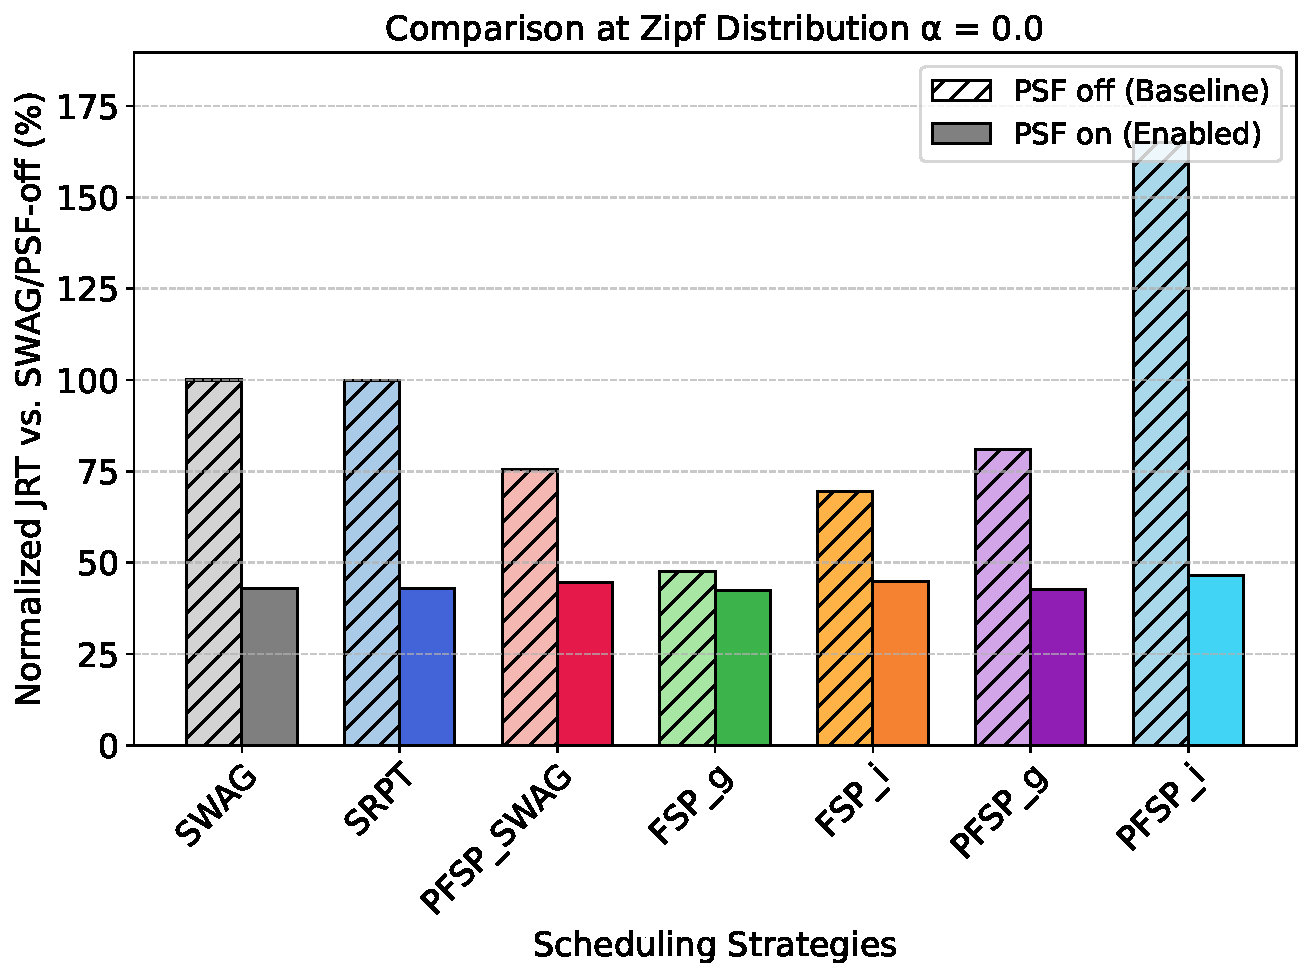
\includegraphics[width=\textwidth]{Image3/PSF_Bar_Ali2017_70_alpha=0.0_dev=0.4.pdf}
        \caption{$\alpha = 0.0$}
    \end{subfigure}
    \hfill
    \begin{subfigure}[b]{0.4\textwidth}
        \centering
        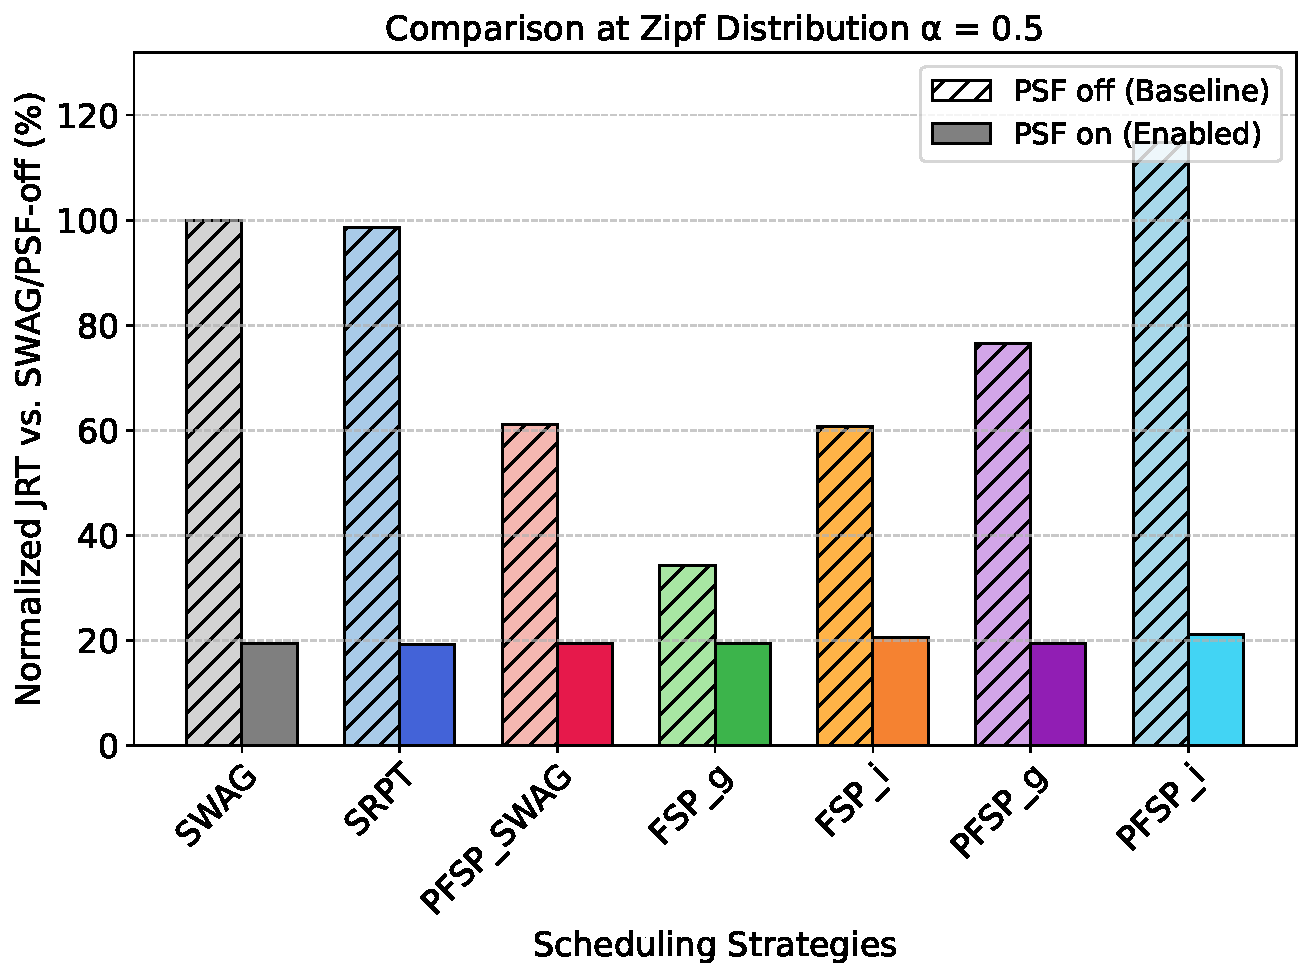
\includegraphics[width=\textwidth]{Image3/PSF_Bar_Ali2017_70_alpha=0.5_dev=0.4.pdf}
        \caption{$\alpha = 0.5$}
    \end{subfigure}
    \vspace{0.8em}
    \begin{subfigure}[b]{0.4\textwidth}
        \centering
        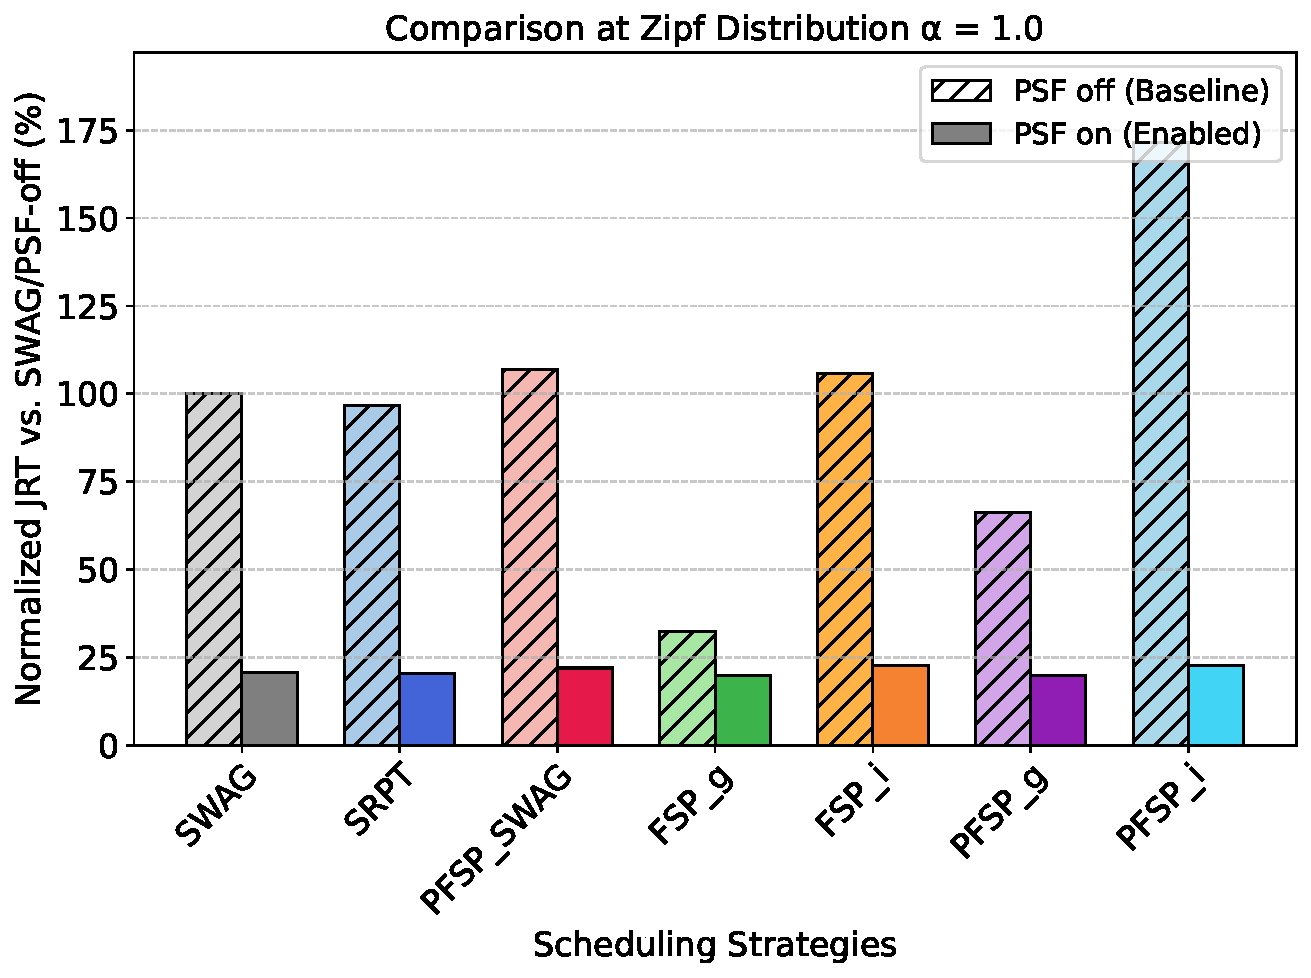
\includegraphics[width=\textwidth]{Image3/PSF_Bar_Ali2017_70_alpha=1.0_dev=0.4.pdf}
        \caption{$\alpha = 1.0$}
    \end{subfigure}
    \hfill
    \begin{subfigure}[b]{0.4\textwidth}
        \centering
        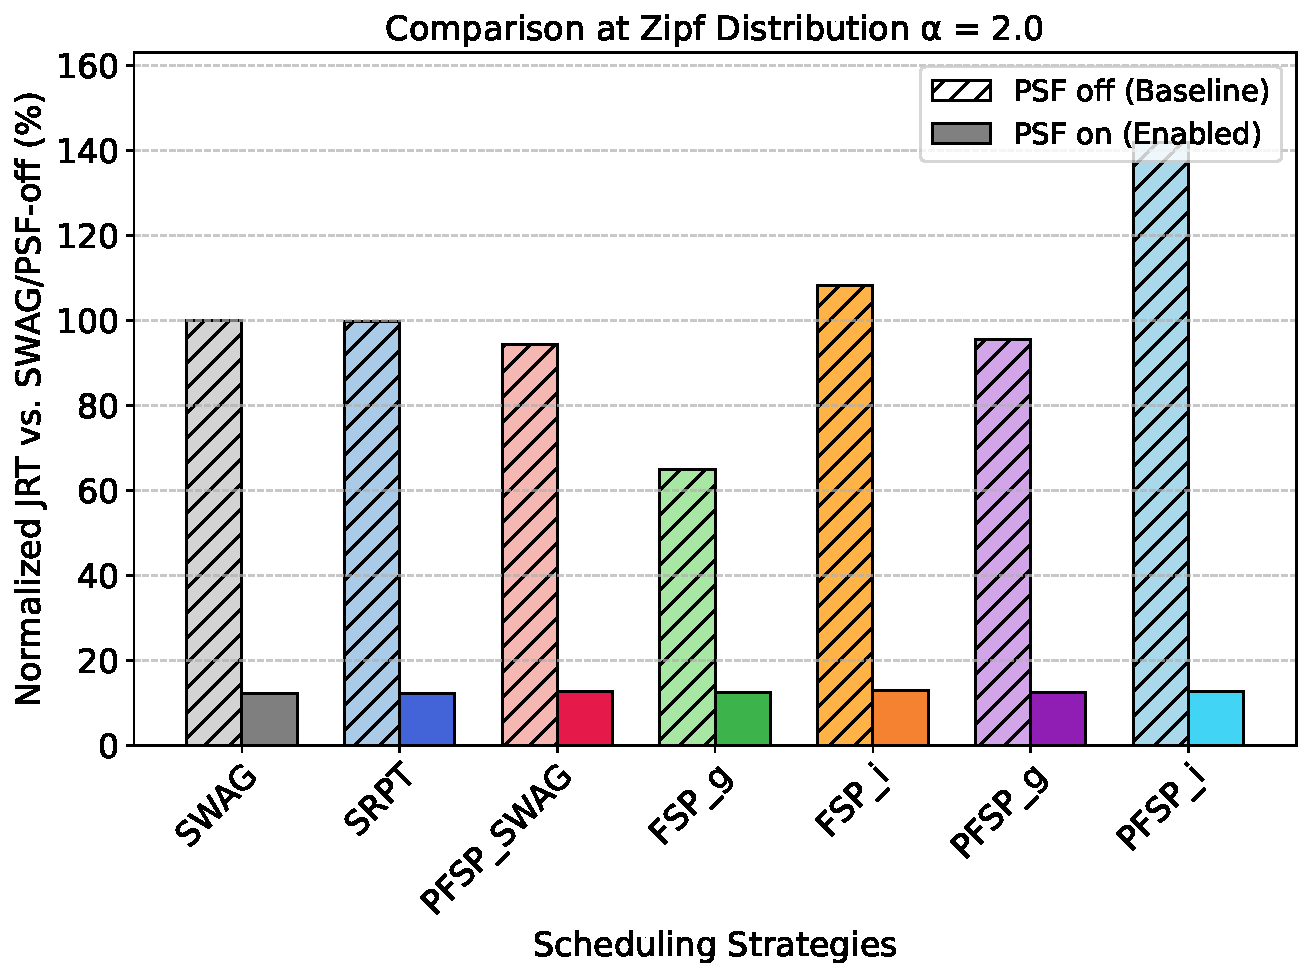
\includegraphics[width=\textwidth]{Image3/PSF_Bar_Ali2017_70_alpha=2.0_dev=0.4.pdf}
        \caption{$\alpha = 2.0$}
    \end{subfigure}

    \caption{Average job response time with/without PSF, 40\% deviation, 70\% utilization, Alibaba 2017}
    \label{fig:JRT_Ali2017_err=0.4}
\end{figure*}

\begin{figure*}[t]
    \centering
    \begin{subfigure}[b]{0.4\textwidth}
        \centering
        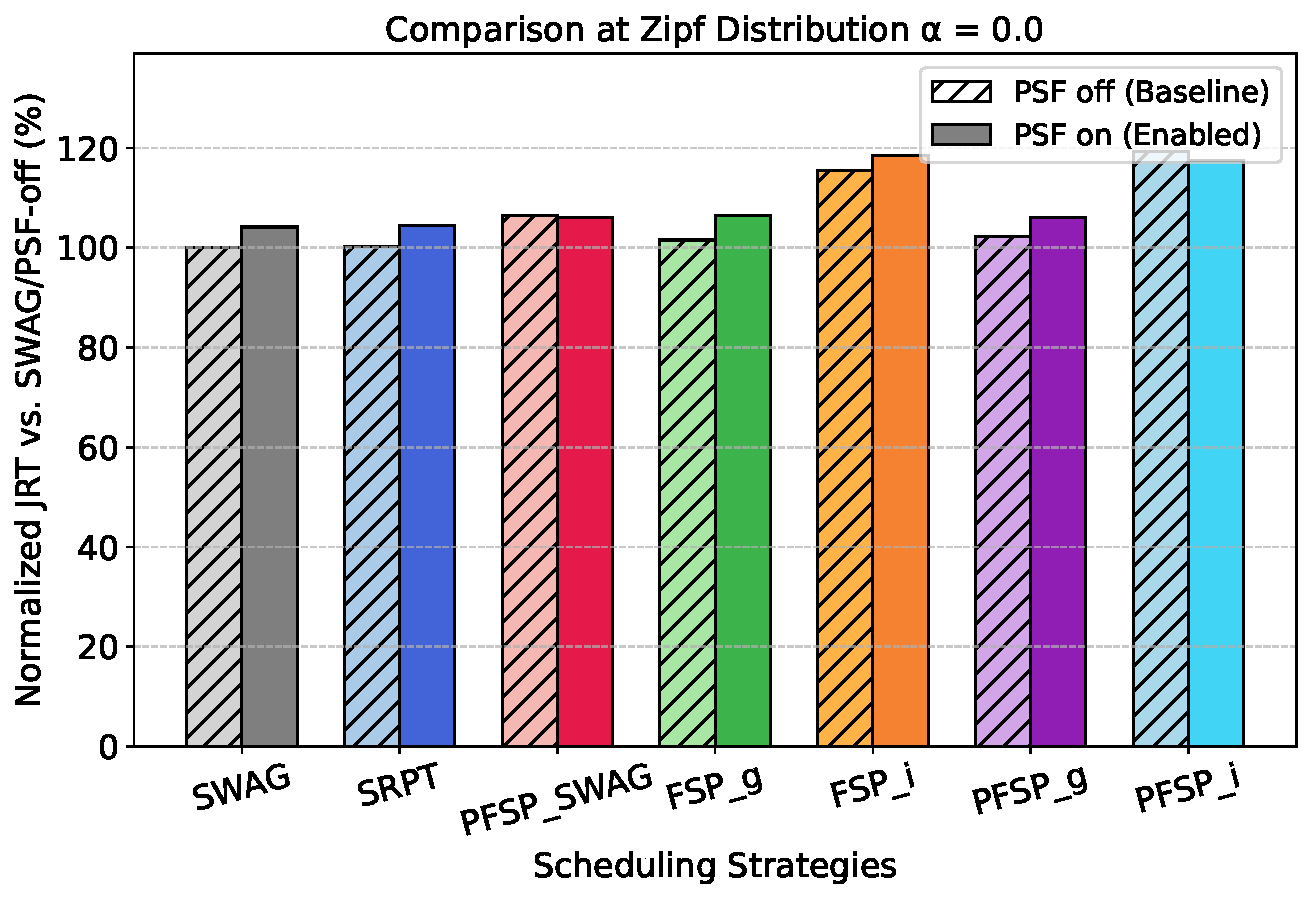
\includegraphics[width=\textwidth]{Image3/PSF_Bar_Ali2018_4_70_alpha=0.0_dev=0.1.pdf}
        \caption{$\alpha = 0.0$}
    \end{subfigure}
    \hfill
    \begin{subfigure}[b]{0.4\textwidth}
        \centering
        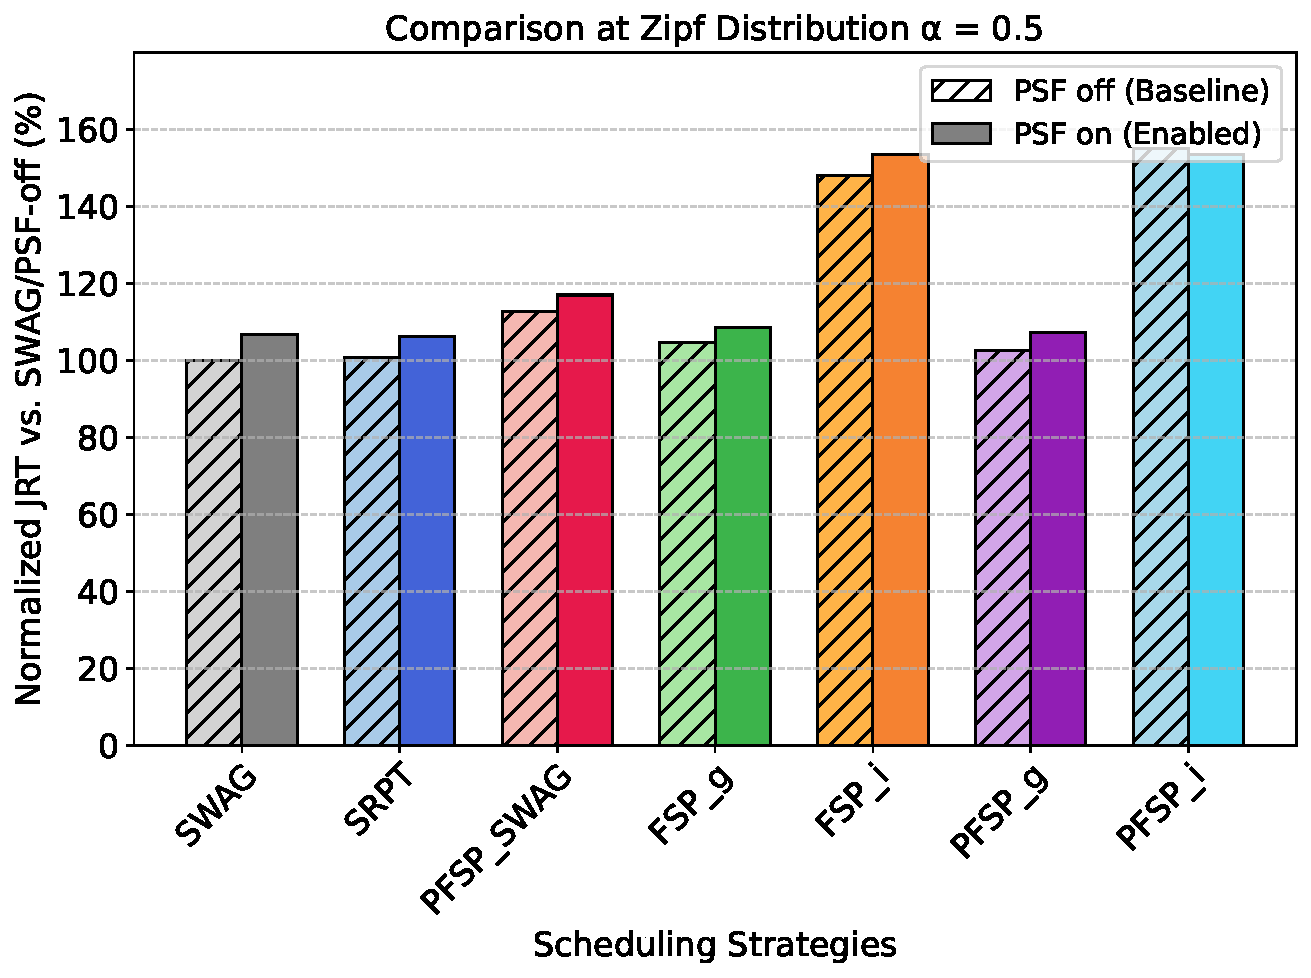
\includegraphics[width=\textwidth]{Image3/PSF_Bar_Ali2018_4_70_alpha=0.5_dev=0.1.pdf}
        \caption{$\alpha = 0.5$}
    \end{subfigure}
    \vspace{0.8em}
    \begin{subfigure}[b]{0.4\textwidth}
        \centering
        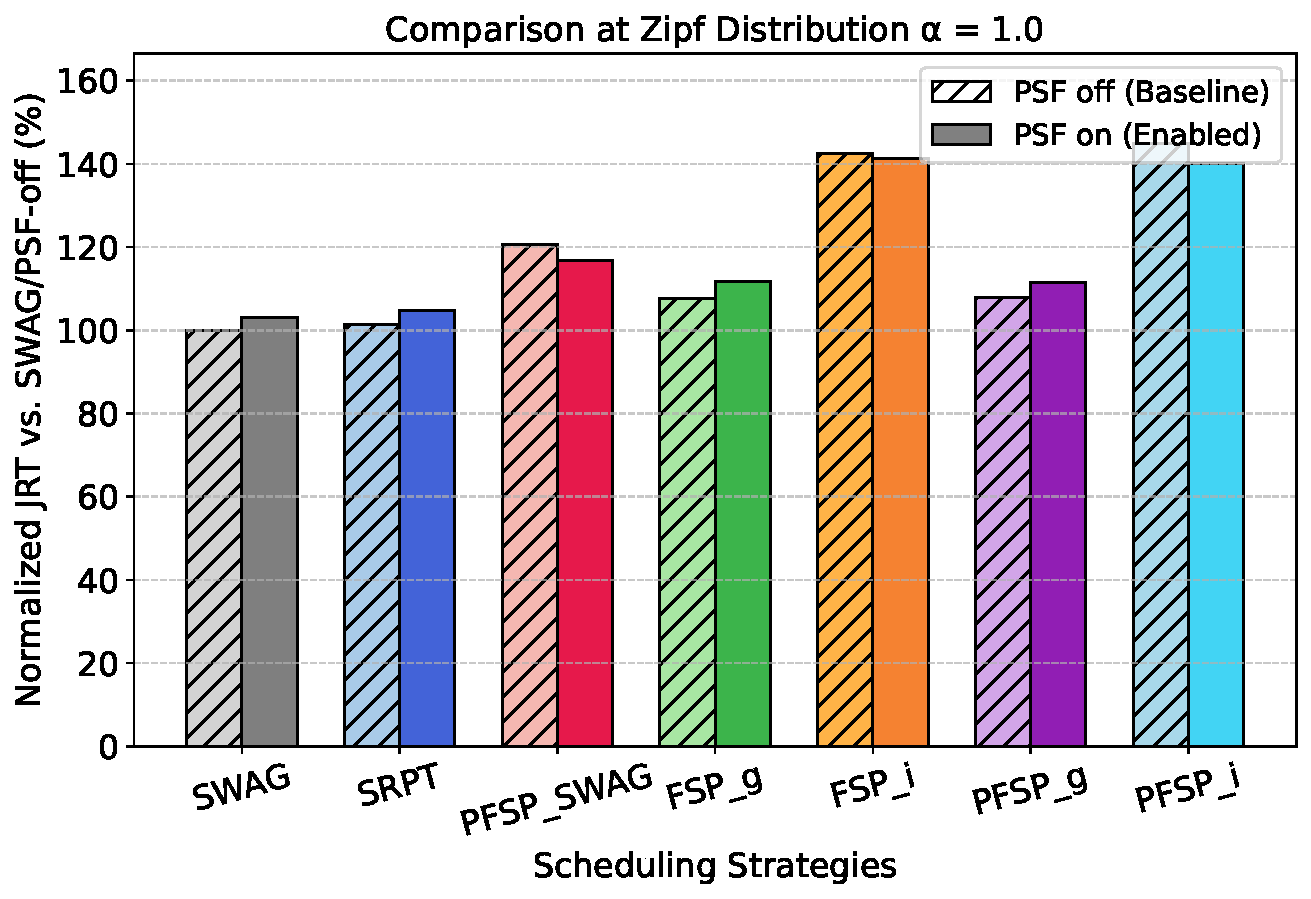
\includegraphics[width=\textwidth]{Image3/PSF_Bar_Ali2018_4_70_alpha=1.0_dev=0.1.pdf}
        \caption{$\alpha = 1.0$}
    \end{subfigure}
    \hfill
    \begin{subfigure}[b]{0.4\textwidth}
        \centering
        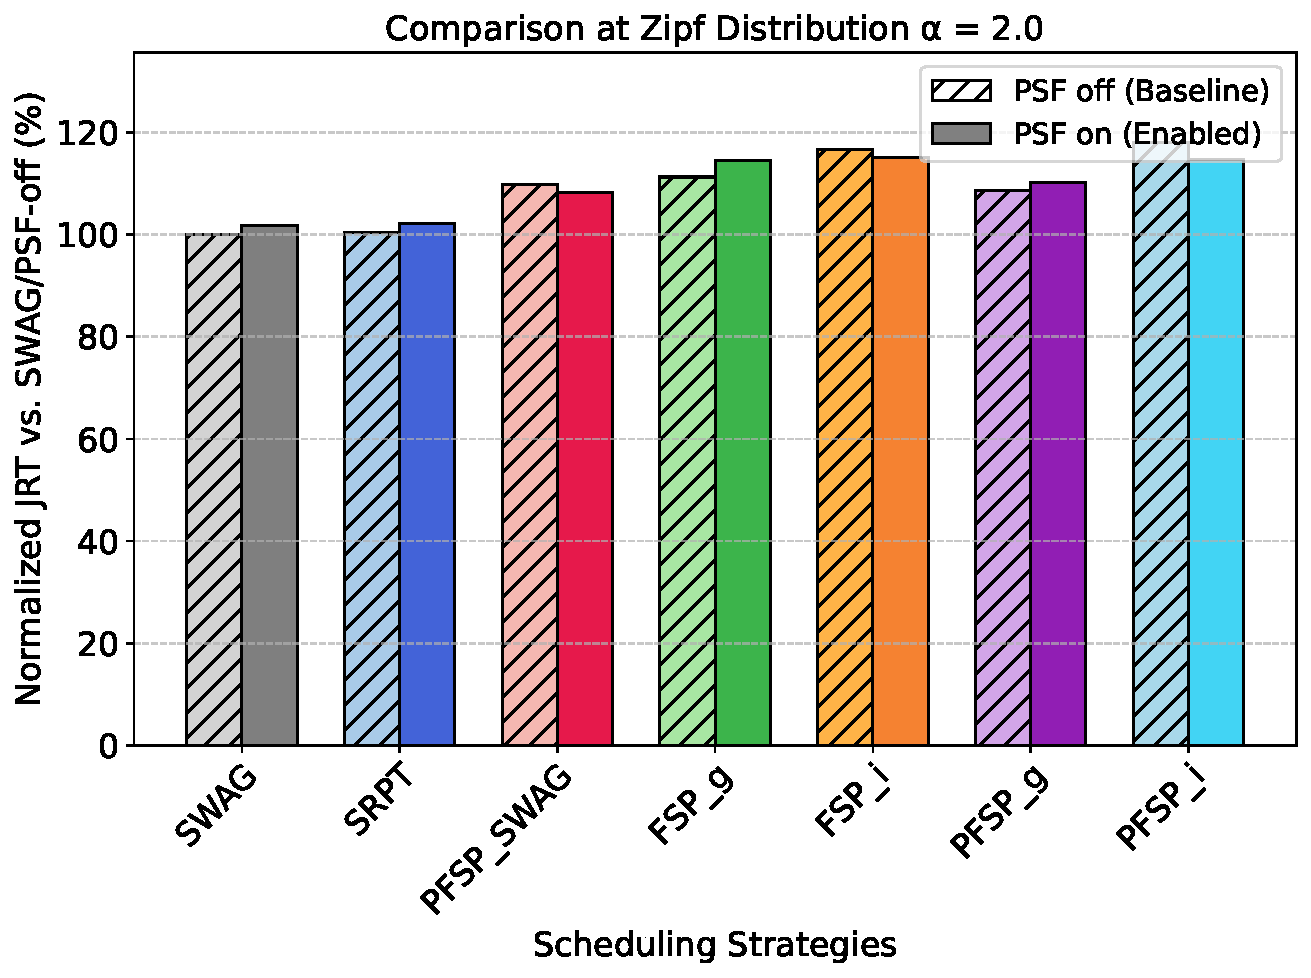
\includegraphics[width=\textwidth]{Image3/PSF_Bar_Ali2018_4_70_alpha=2.0_dev=0.1.pdf}
        \caption{$\alpha = 2.0$}
    \end{subfigure}

    \caption{Average job response time with/without PSF, 10\% deviation, 70\% utilization, Alibaba 2018}
    \label{fig:JRT_Ali2018_err=0.1}
\end{figure*}

\begin{figure*}[t]
    \centering
    \begin{subfigure}[b]{0.4\textwidth}
        \centering
        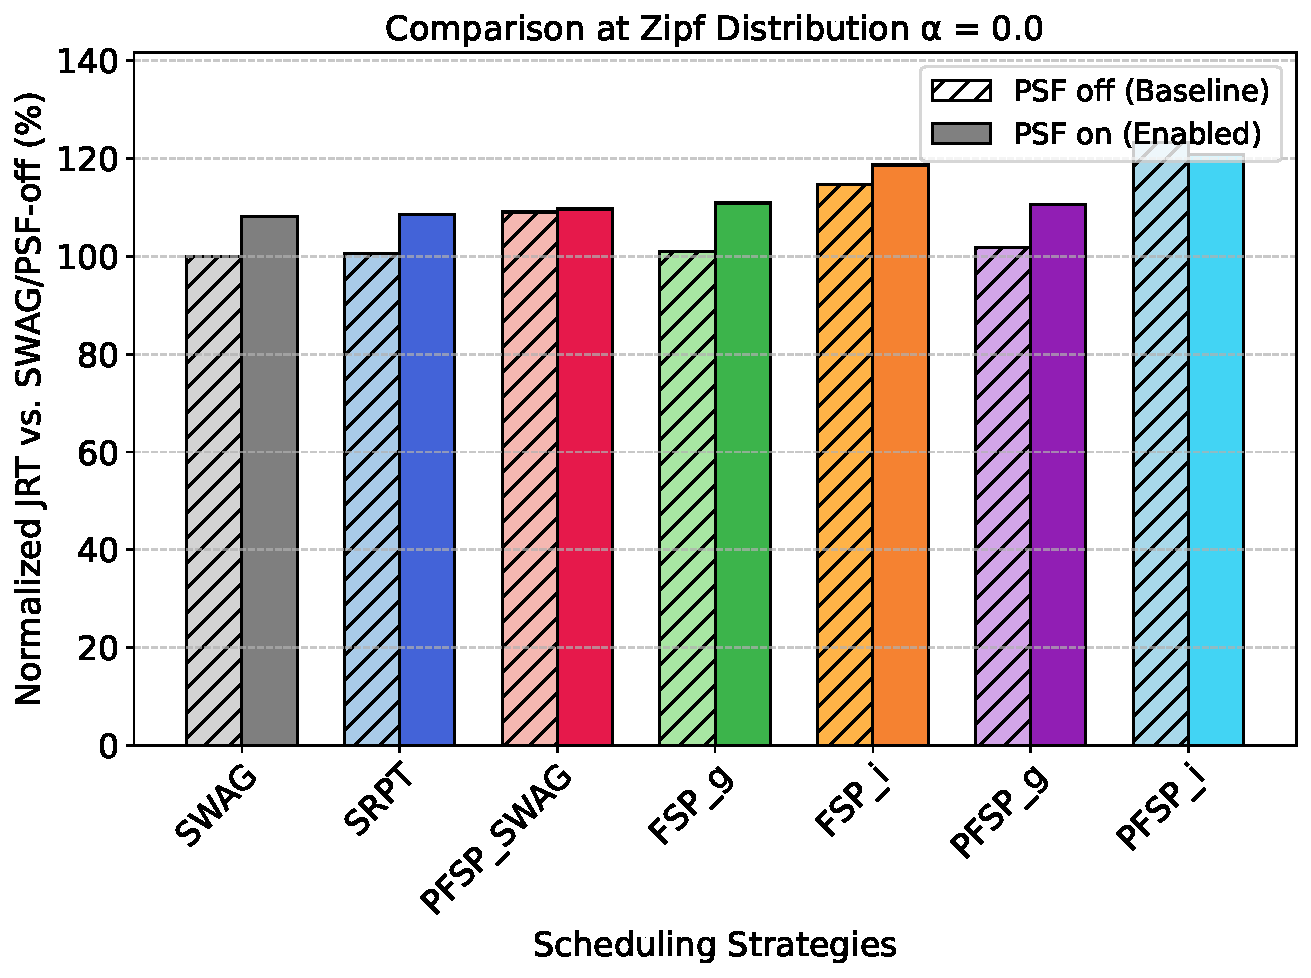
\includegraphics[width=\textwidth]{Image3/PSF_Bar_Ali2018_4_70_alpha=0.0_dev=0.2.pdf}
        \caption{$\alpha = 0.0$}
    \end{subfigure}
    \hfill
    \begin{subfigure}[b]{0.4\textwidth}
        \centering
        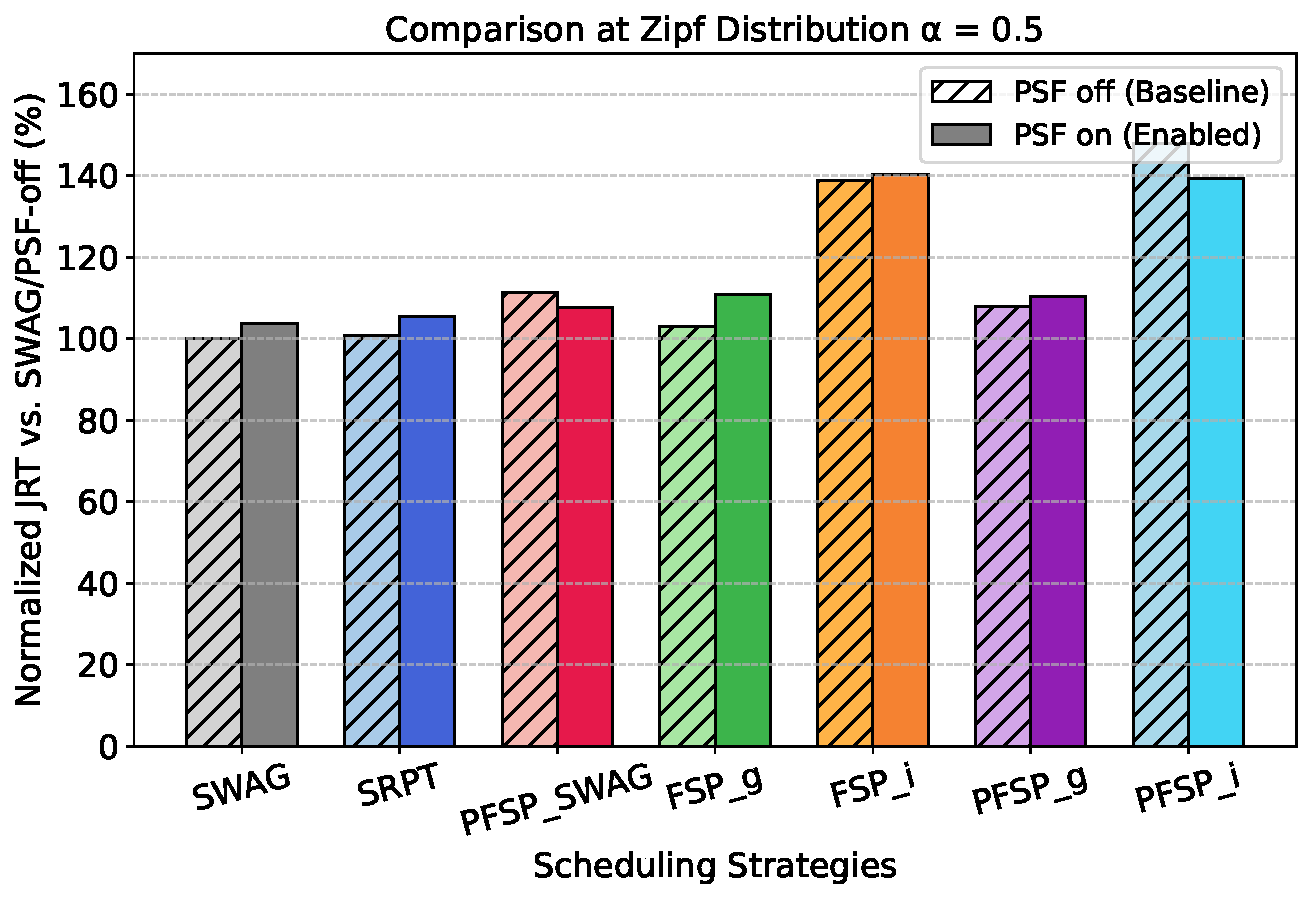
\includegraphics[width=\textwidth]{Image3/PSF_Bar_Ali2018_4_70_alpha=0.5_dev=0.2.pdf}
        \caption{$\alpha = 0.5$}
    \end{subfigure}
    \vspace{0.8em}
    \begin{subfigure}[b]{0.4\textwidth}
        \centering
        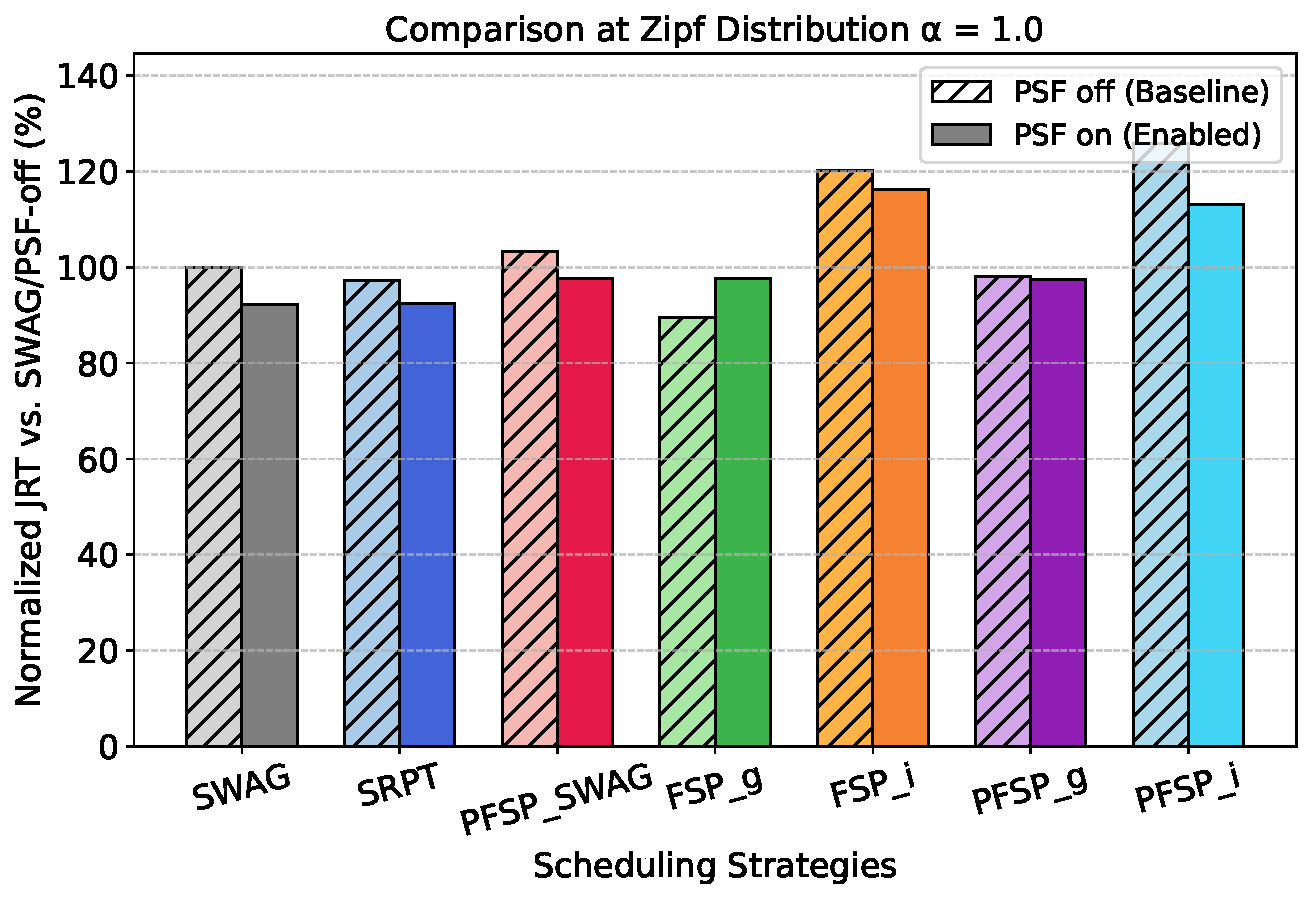
\includegraphics[width=\textwidth]{Image3/PSF_Bar_Ali2018_4_70_alpha=1.0_dev=0.2.pdf}
        \caption{$\alpha = 1.0$}
    \end{subfigure}
    \hfill
    \begin{subfigure}[b]{0.4\textwidth}
        \centering
        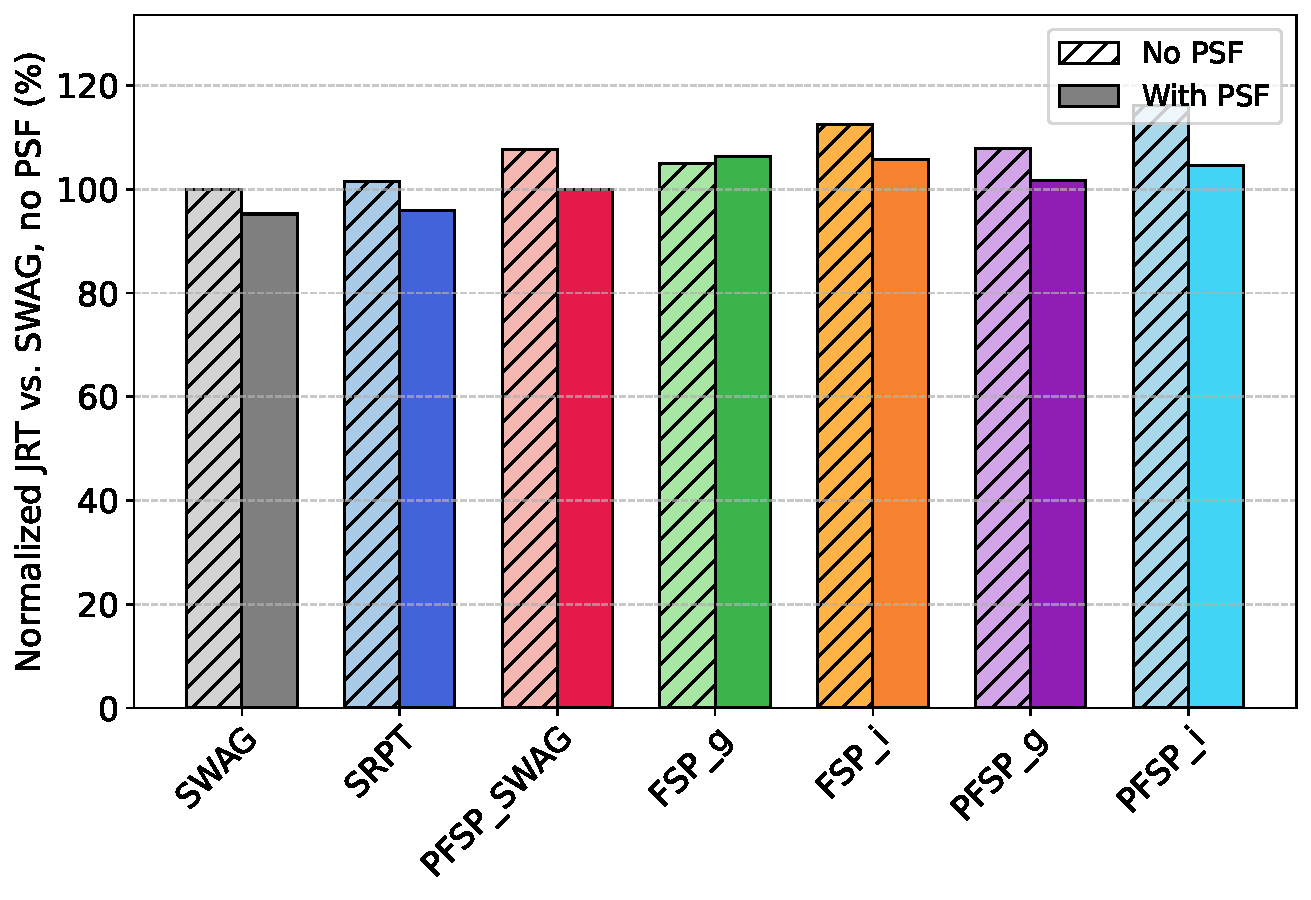
\includegraphics[width=\textwidth]{Image3/PSF_Bar_Ali2018_4_70_alpha=2.0_dev=0.2.pdf}
        \caption{$\alpha = 2.0$}
    \end{subfigure}

    \caption{Average job response time with/without PSF, 20\% deviation, 70\% utilization, Alibaba 2018}
    \label{fig:JRT_Ali2018_err=0.2}
\end{figure*}

\begin{figure*}[t]
    \centering
    \begin{subfigure}[b]{0.4\textwidth}
        \centering
        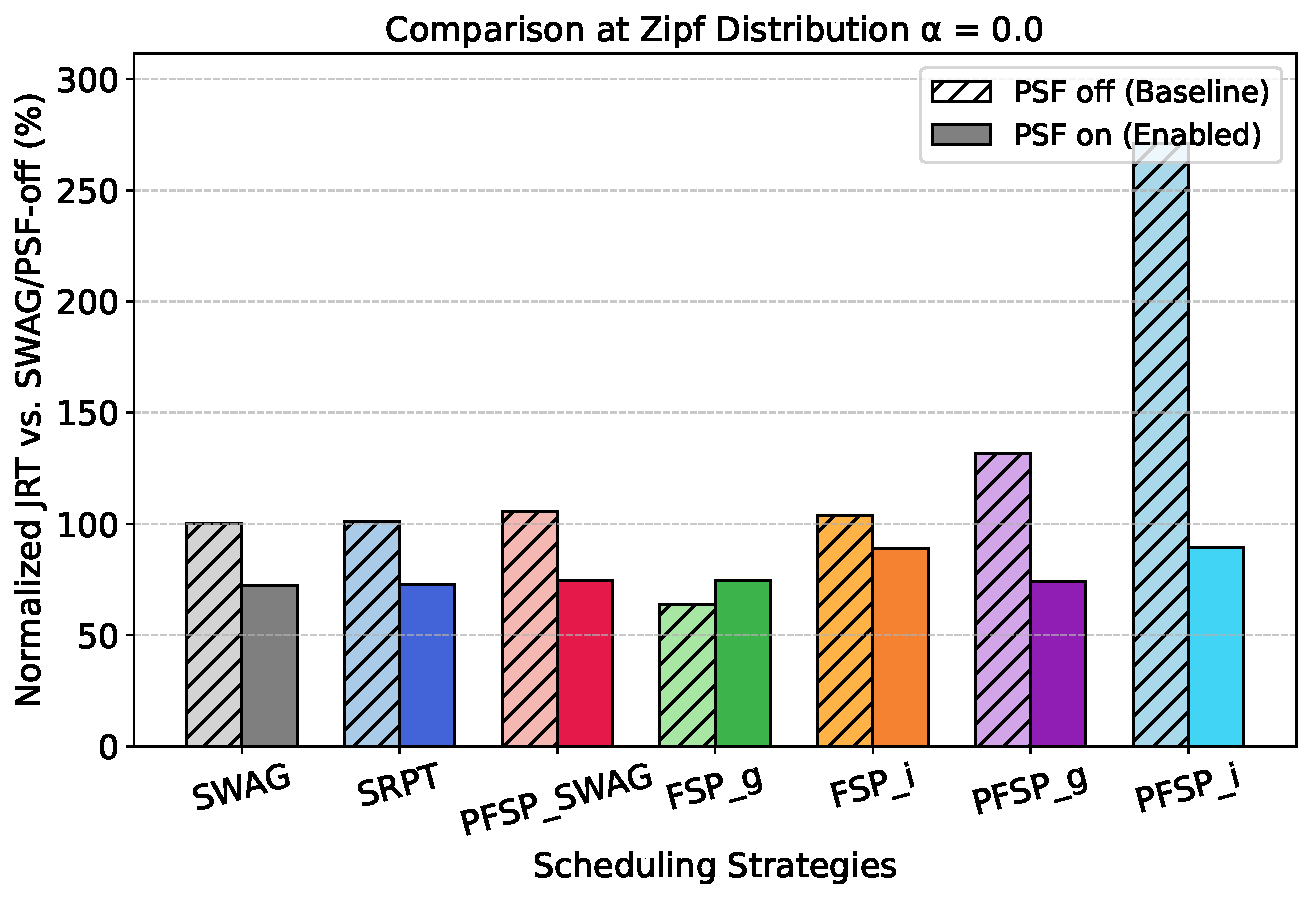
\includegraphics[width=\textwidth]{Image3/PSF_Bar_Ali2018_4_70_alpha=0.0_dev=0.3.pdf}
        \caption{$\alpha = 0.0$}
    \end{subfigure}
    \hfill
    \begin{subfigure}[b]{0.4\textwidth}
        \centering
        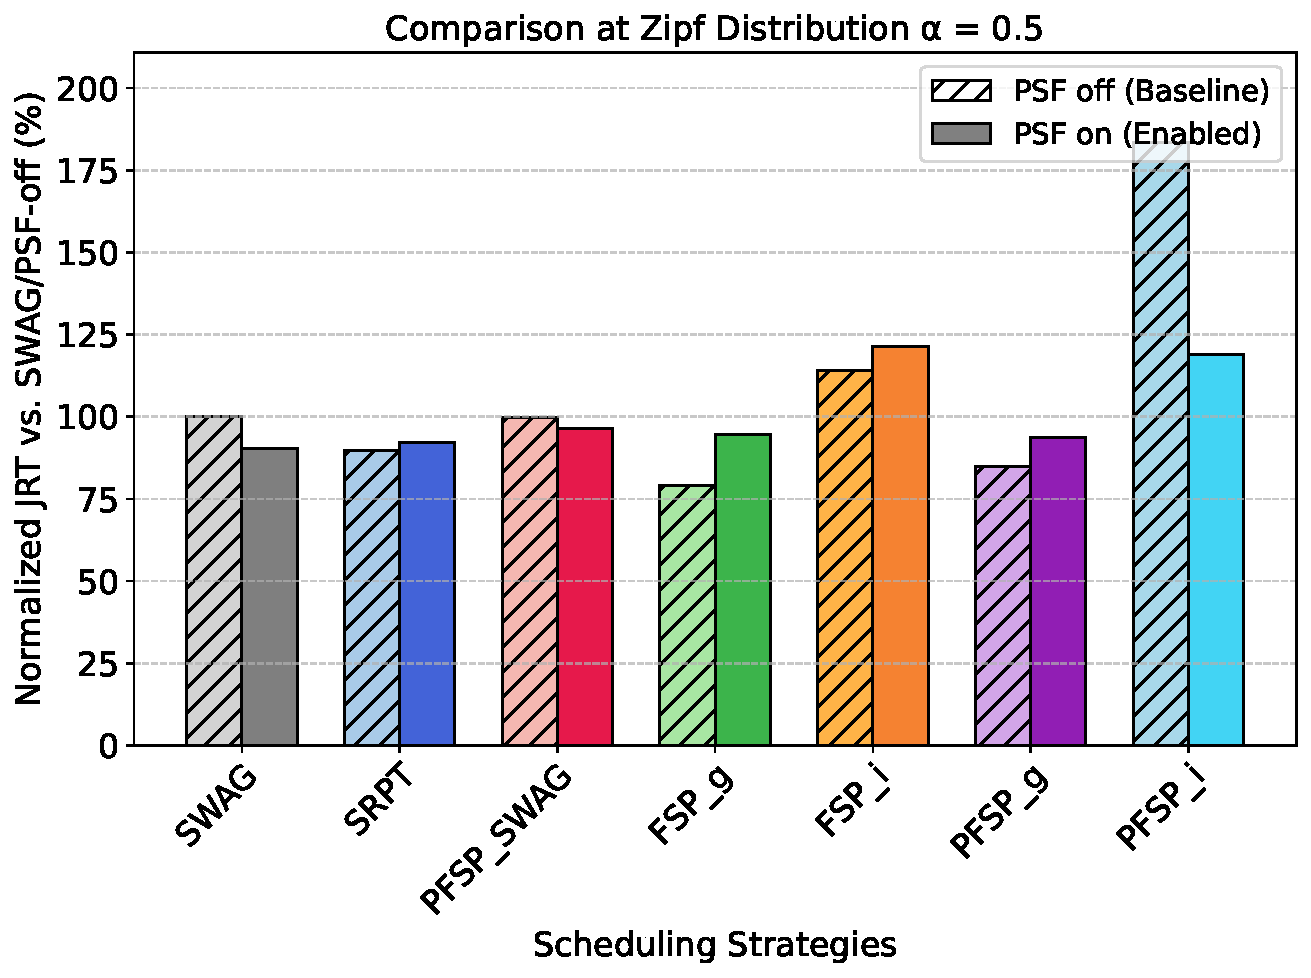
\includegraphics[width=\textwidth]{Image3/PSF_Bar_Ali2018_4_70_alpha=0.5_dev=0.3.pdf}
        \caption{$\alpha = 0.5$}
    \end{subfigure}
    \vspace{0.8em}
    \begin{subfigure}[b]{0.4\textwidth}
        \centering
        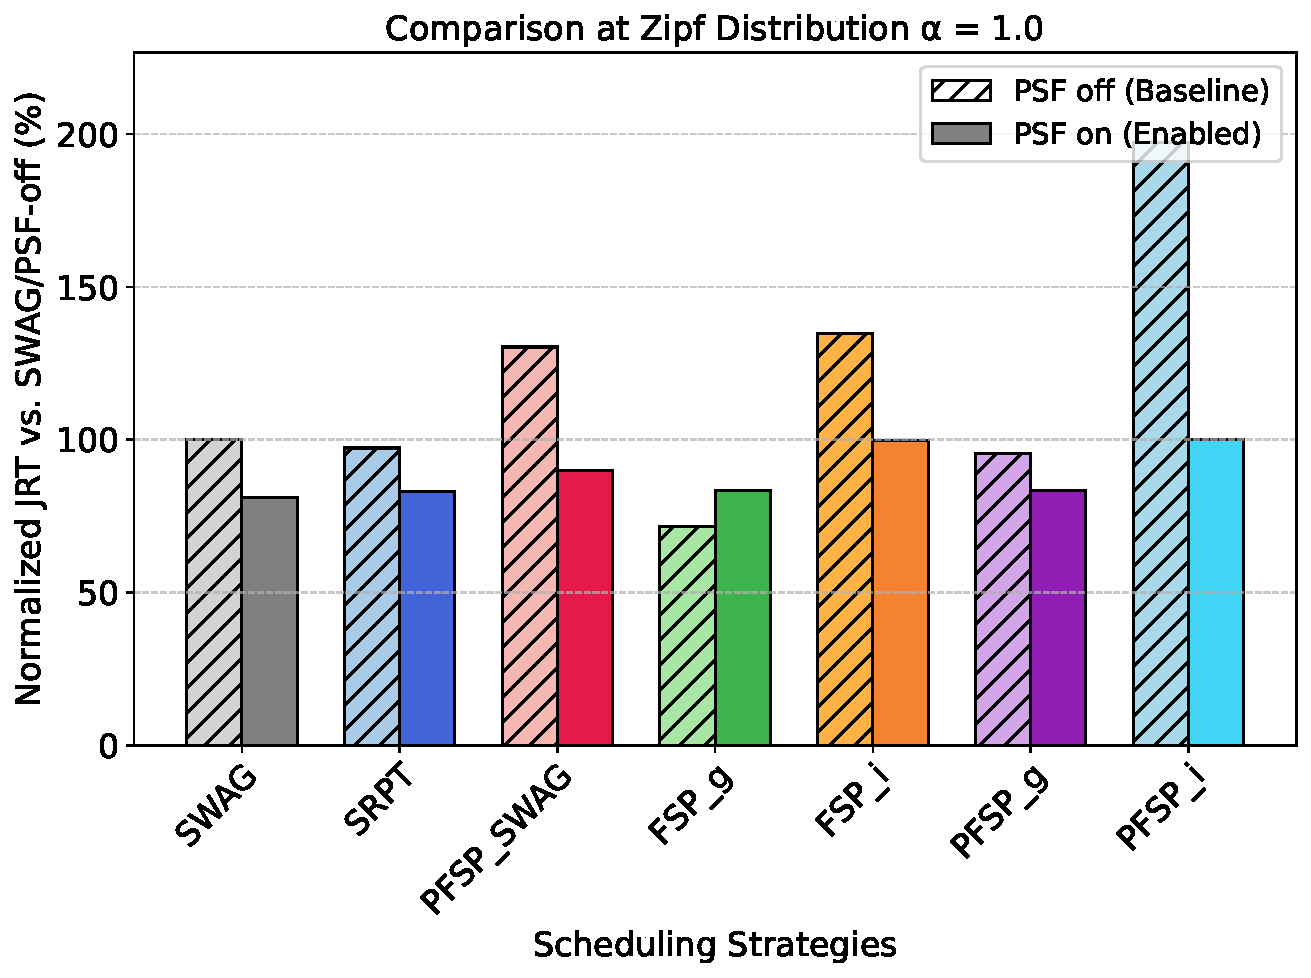
\includegraphics[width=\textwidth]{Image3/PSF_Bar_Ali2018_4_70_alpha=1.0_dev=0.3.pdf}
        \caption{$\alpha = 1.0$}
    \end{subfigure}
    \hfill
    \begin{subfigure}[b]{0.4\textwidth}
        \centering
        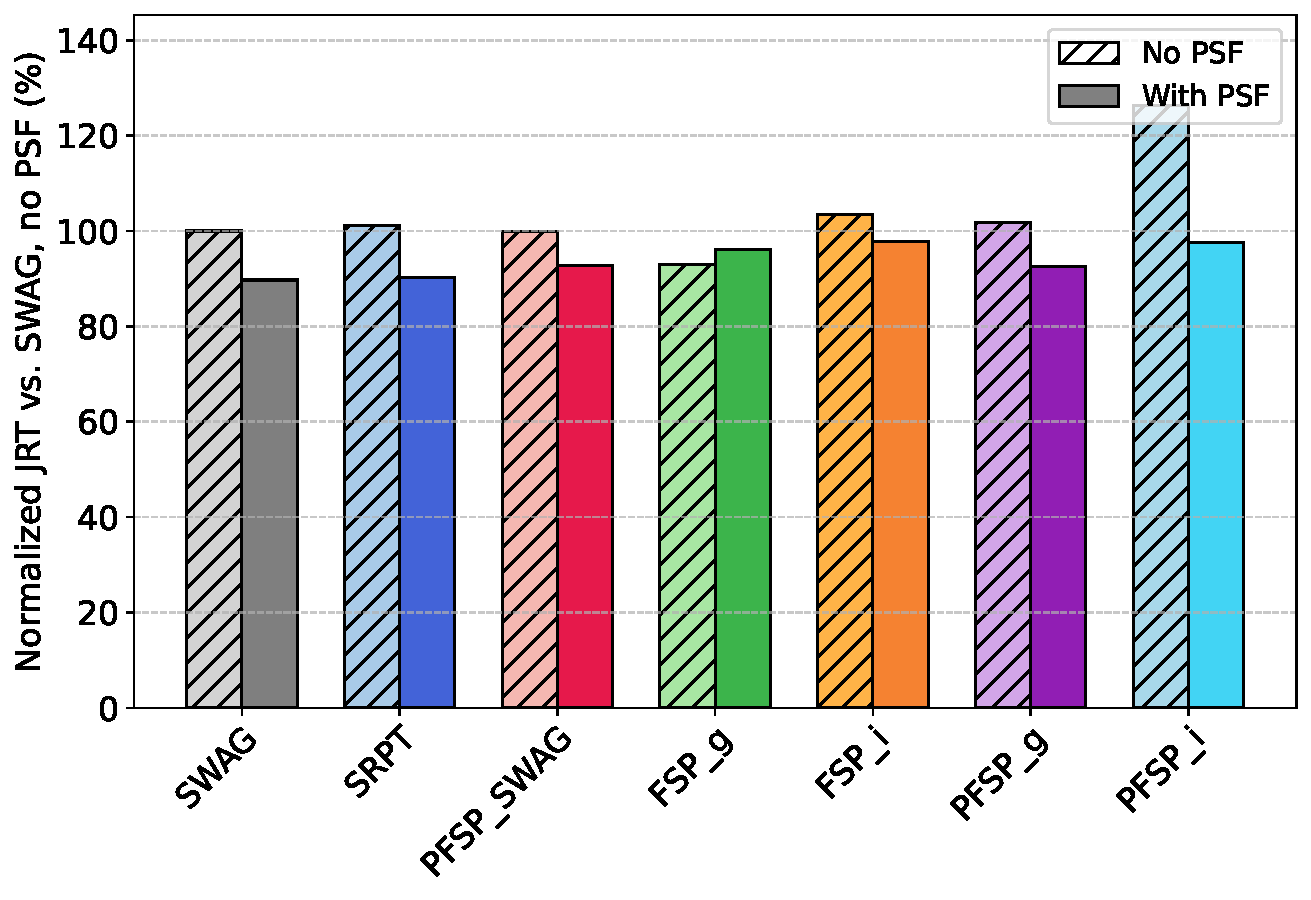
\includegraphics[width=\textwidth]{Image3/PSF_Bar_Ali2018_4_70_alpha=2.0_dev=0.3.pdf}
        \caption{$\alpha = 2.0$}
    \end{subfigure}

    \caption{Average job response time with/without PSF, 30\% deviation, 70\% utilization, Alibaba 2018}
    \label{fig:JRT_Ali2018_err=0.3}
\end{figure*}

\begin{figure*}[t]
    \centering
    \begin{subfigure}[b]{0.4\textwidth}
        \centering
        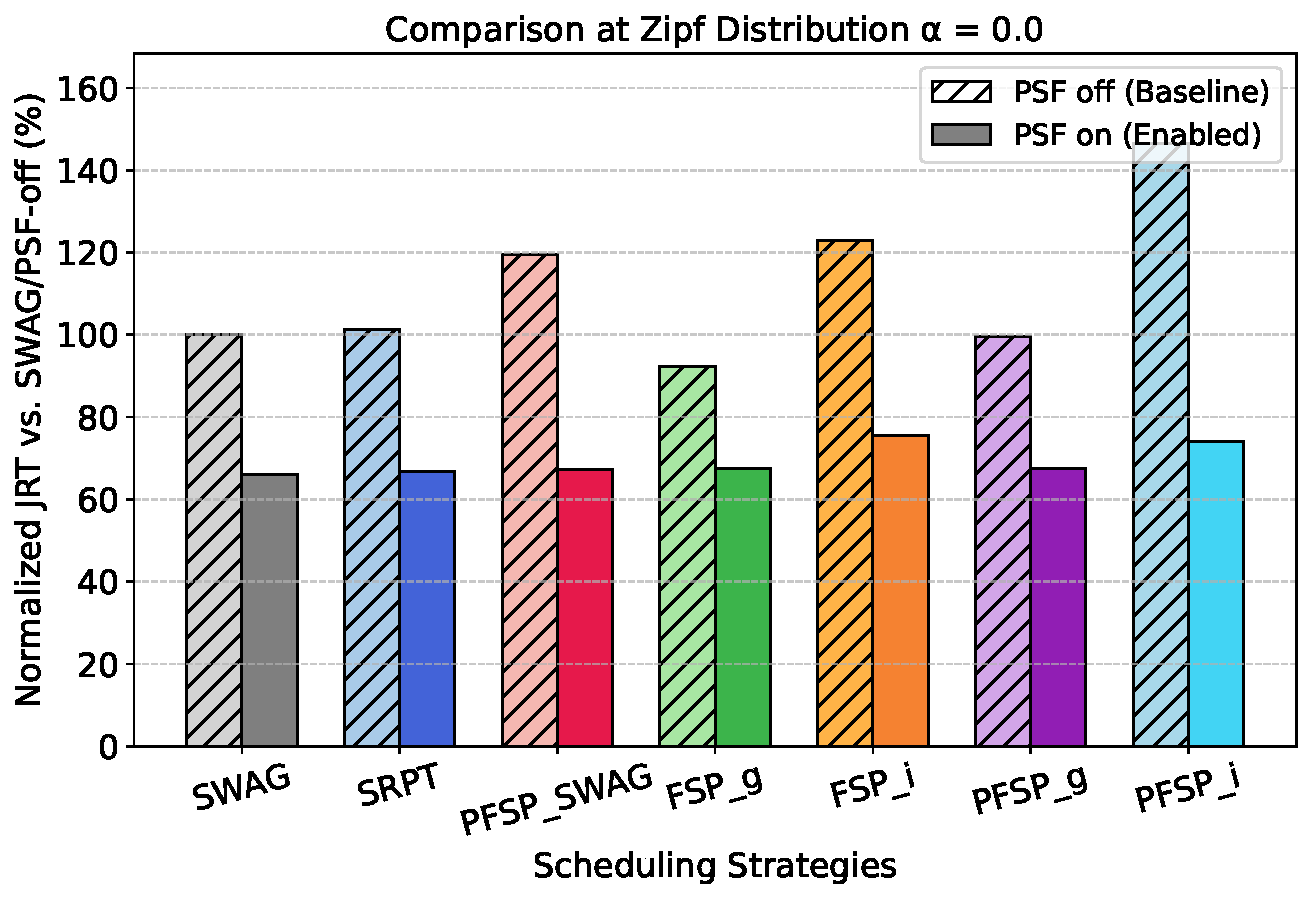
\includegraphics[width=\textwidth]{Image3/PSF_Bar_Ali2018_4_70_alpha=0.0_dev=0.4.pdf}
        \caption{$\alpha = 0.0$}
    \end{subfigure}
    \hfill
    \begin{subfigure}[b]{0.4\textwidth}
        \centering
        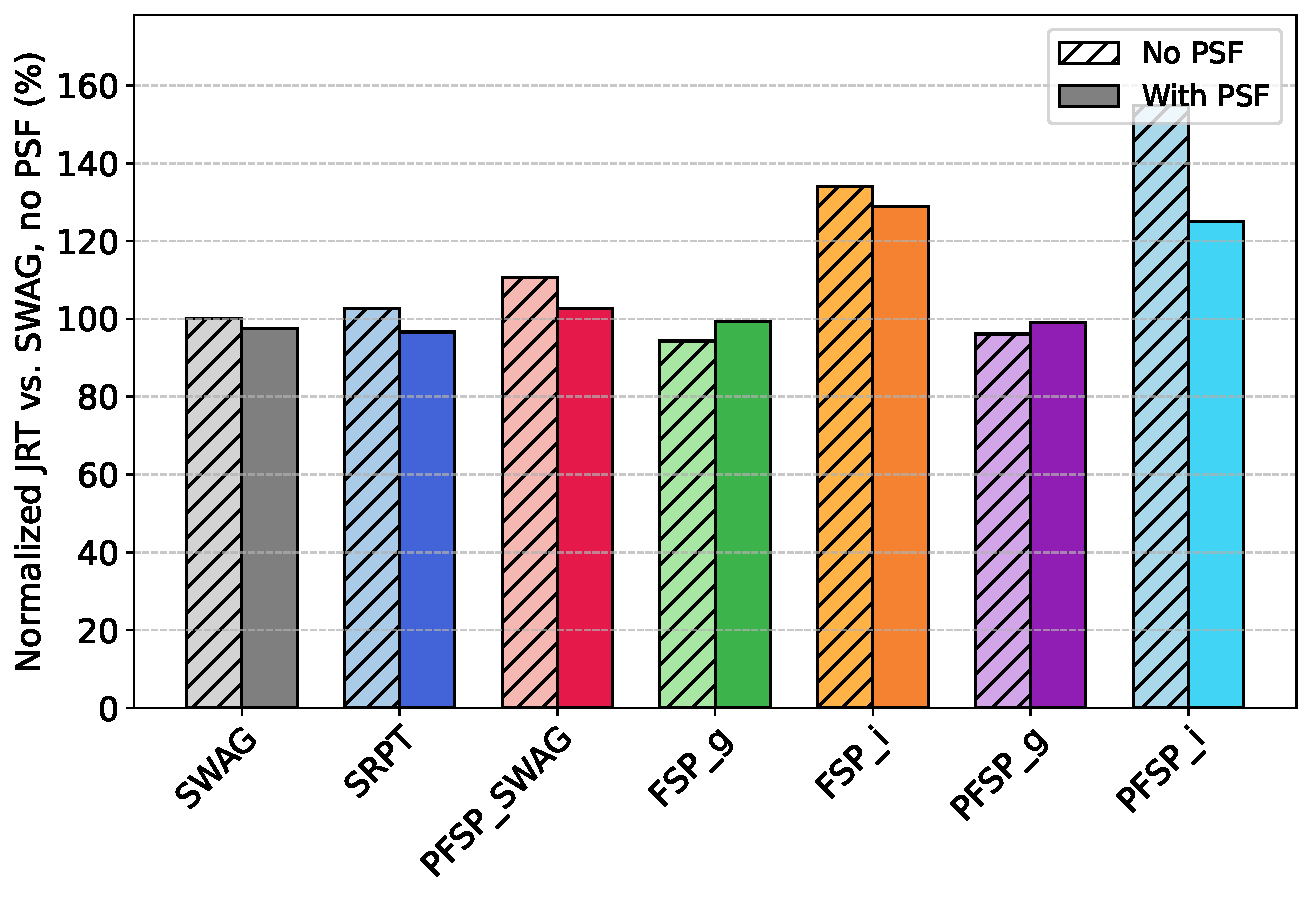
\includegraphics[width=\textwidth]{Image3/PSF_Bar_Ali2018_4_70_alpha=0.5_dev=0.4.pdf}
        \caption{$\alpha = 0.5$}
    \end{subfigure}
    \vspace{0.8em}
    \begin{subfigure}[b]{0.4\textwidth}
        \centering
        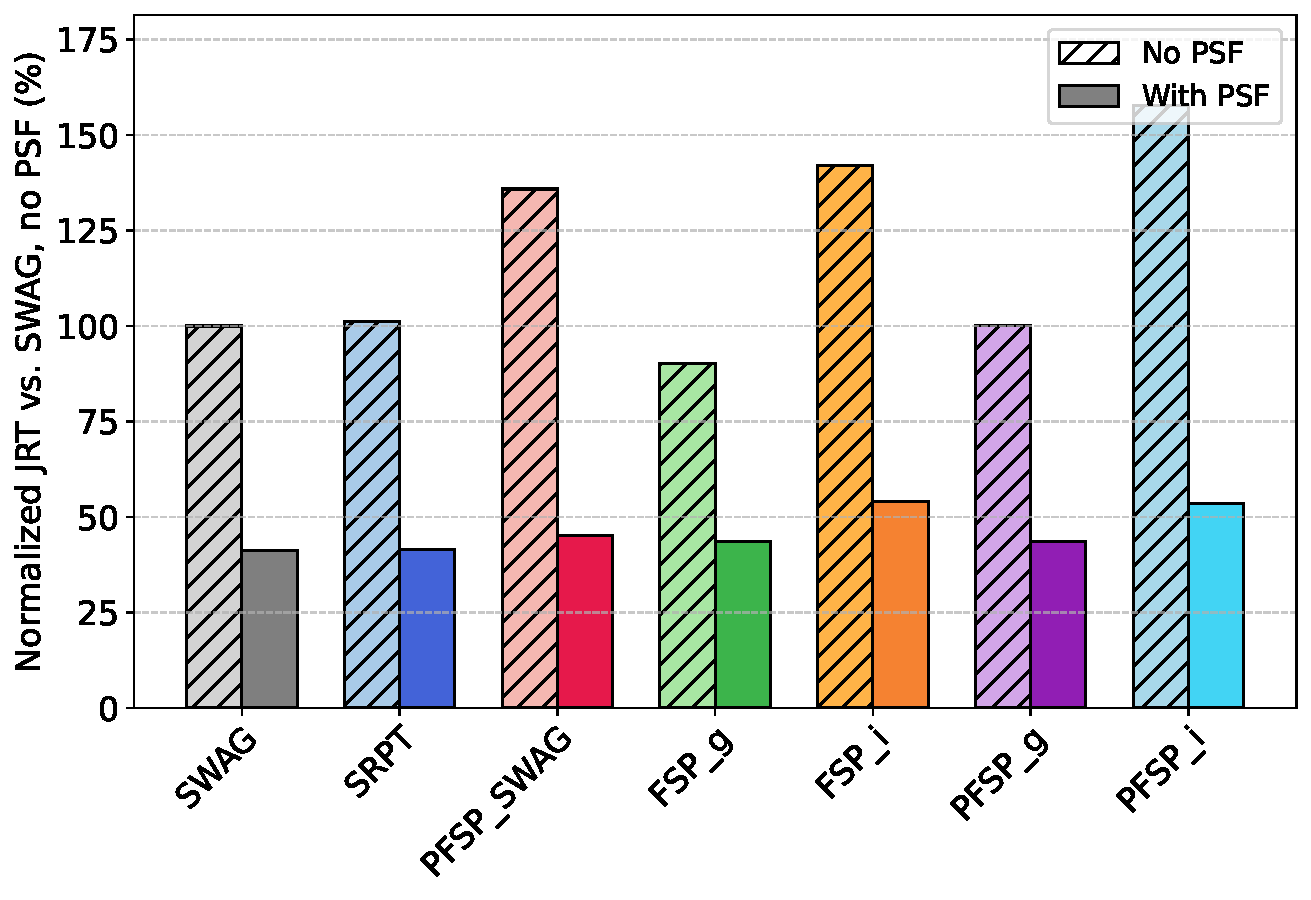
\includegraphics[width=\textwidth]{Image3/PSF_Bar_Ali2018_4_70_alpha=1.0_dev=0.4.pdf}
        \caption{$\alpha = 1.0$}
    \end{subfigure}
    \hfill
    \begin{subfigure}[b]{0.4\textwidth}
        \centering
        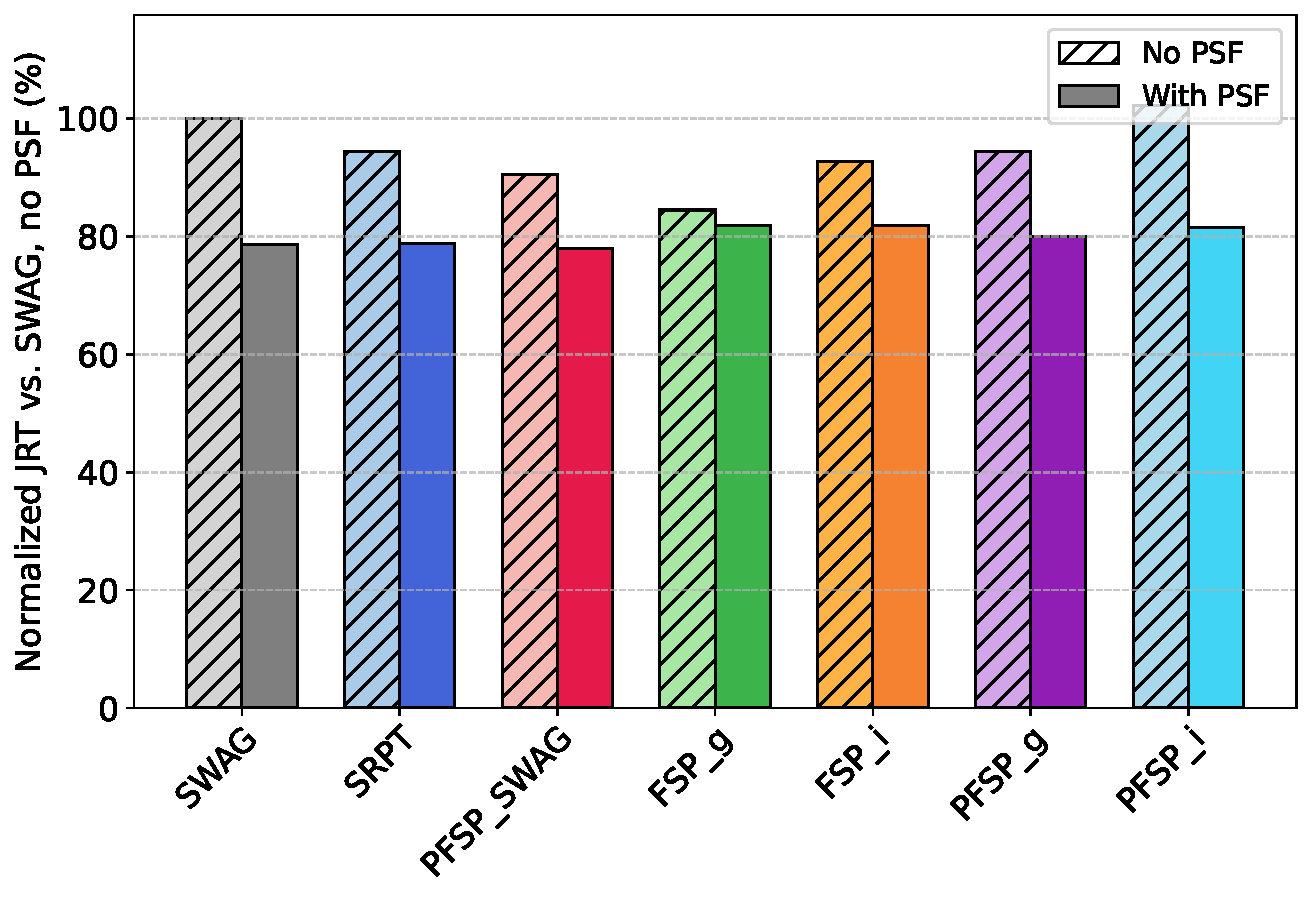
\includegraphics[width=\textwidth]{Image3/PSF_Bar_Ali2018_4_70_alpha=2.0_dev=0.4.pdf}
        \caption{$\alpha = 2.0$}
    \end{subfigure}

    \caption{Average job response time with/without PSF, 40\% deviation, 70\% utilization, Alibaba 2018}
    \label{fig:JRT_Ali2018_err=0.4}
\end{figure*}

Figures \ref{fig:JRT_Ali2017_err=0.1} through \ref{fig:JRT_Ali2018_err=0.4} illustrate the average job response time  under different deviations of job load estimations for both datasets. To facilitate comparison, the response time of the baseline SWAG policy—without the PSF mechanism—is normalized to $100\%$, with all other policies expressed relative to this baseline. Overall, the performance difference between policies with and without the PSF mechanism remains minor across most scenarios. However, in certain cases (e.g., Figure \ref{fig:JRT_Ali2017_err=0.4}), integrating the PSF mechanism yields a substantial reduction in average job response time across all evaluated scheduling policies. In conclusion, incorporating the PSF mechanism into the evaluated scheduling policies significantly mitigates PS deadline violations while maintaining comparable or superior average job response times. 


\section{Summary}
\label{sec:conclusion3}

In this chapter, we investigated how to achieve the dual objective between efficiency and long-term fairness in distributed job execution by extending the theory of protective scheduling in the single-site case. We established the distributed slack system to help judge the system protectiveness using two perspectives: the Global Slack ($GS$) scheme and the Independent Slack ($IS$) scheme. Through theoretical analysis, we proved that dynamic job arrivals inherently prevent global order-based policies from guaranteeing strict protectiveness under the $GS$ scheme. To overcome this dilemma, we proposed PFSP\_x, a novel heuristic scheduling framework that adopts the $IS$ scheme to ensure protectiveness while approximating a hint job order derived by any efficiency-targeted policies. We also developed a series of extension policies based on the single-site policies FSP, PFSP and OFSP as the baselines. Extensive trace-driven simulations using Alibaba cluster datasets demonstrated that our proposed PFSP\_SWAG policy achieves the highest job processing efficiency among all strictly protective policies evaluated. Furthermore, the extension policy PFSP\_g under the $GS$ scheme is shown capable of delivering average job response times comparable to efficiency-targeted policies with negligible fairness violations. Ultimately, these complementary strategies equip distributed systems to flexibly navigate the delicate trade-off between job processing efficiency and long-term fairness.
%In conclusion, we present two primary scheduling policies, by which the distributed system is empowered to flexibly adapt to different system requirements, effectively balancing the delicate trade-off between job processing efficiency and long-term job fairness.
